\documentclass[a4paper,12pt]{report}
\usepackage[hyphens]{url}
\usepackage[colorlinks=true,allcolors=blueLink]{hyperref}
\usepackage[margin=2cm]{geometry}
\usepackage{abstract}
\usepackage{polyglossia}

\usepackage[binary-units=true,detect-all,group-separator={,},group-minimum-digits=4]{siunitx}
\usepackage{amsmath,amssymb,amsthm}
\usepackage[round]{natbib}
\usepackage{algorithmic}
\usepackage{algorithm}
\usepackage{bm}
\usepackage{booktabs}
\usepackage{graphicx}
\usepackage{multirow}
\usepackage{adjustbox}
\usepackage{multicol}
\usepackage{pgf}
\usepackage{pgfplots}
\usepackage{tikz}
\usepackage{xcolor}
\usepackage{subcaption}
\usepackage{listings}
\usepackage{threeparttable}
\usepackage{listings}

\bibliographystyle{plainnat}

\setmainlanguage{english}
\setotherlanguage{french}

\theoremstyle{definition}
\newtheorem{definition}{Definition}[section]

\usetikzlibrary{arrows,automata,calc,decorations.pathreplacing,positioning,shapes,snakes}

\tikzset{%
  arrow/.style={thick,-stealth},
  edge/.style={midway,sloped,above},
  entity/.style={circle,draw},
  label/.style={yshift=0.2cm},
}

\definecolor{eclipseComment}{RGB}{63,127,95}
\definecolor{eclipseKeywords}{RGB}{127,0,85}
\definecolor{eclipseStrings}{RGB}{42,0.0,255}

\definecolor{blueLink}{HTML}{180CAD}
\definecolor{dark}{HTML}{7B7D7B}
\definecolor{grey}{HTML}{C6C7C6}
\definecolor{green}{HTML}{789437}
\definecolor{blue}{HTML}{377894}
\definecolor{red}{HTML}{943778}
\definecolor{mygreen}{HTML}{bdd7d6}
\definecolor{myred}{HTML}{dec3d6}

\definecolor{myyellow}{HTML}{d6dec3}
\definecolor{mygreen}{HTML}{c3ded9}
\definecolor{myblue}{HTML}{c3d6de}
\definecolor{darkBlue}{HTML}{5f8ba8}
\definecolor{mypurple}{HTML}{c3c9de}
\definecolor{darkPurple}{HTML}{485684}
\definecolor{myyellow}{HTML}{DED8C3}
\definecolor{mybrown}{HTML}{DEC3C9}
\definecolor{darkRed}{HTML}{844871}

\definecolor{dark}{HTML}{7B7D7B}
\definecolor{eclipseComment}{RGB}{63,127,95}
\definecolor{eclipseKeywords}{RGB}{127,0,85}
\definecolor{eclipseStrings}{RGB}{42,0.0,255}
\definecolor{grey}{HTML}{C6C7C6}

\definecolor{brown}{HTML}{945337}
\definecolor{medimumBlue}{HTML}{60A8A1}
\definecolor{yellow}{HTML}{938136}

\definecolor{darkGreen}{HTML}{499336}
\definecolor{lightGreen}{HTML}{779336}
\definecolor{mediumGreen}{HTML}{369352}

\lstset{
  language=Python,
  backgroundcolor=\color{grey!10},
  basicstyle=\fontsize{10}{10}\selectfont\ttfamily,
  breaklines=true,
  commentstyle=\color{eclipseComment},
  frame=lines,
  keywordstyle=\color{eclipseKeywords}\bfseries,
  morekeywords={get\_balance,get\_estaking,get\_gtime,get\_lstaking,get\_mcost,get\_pcost,IP1,fmincon,inf,linprog,ones},
  stringstyle=\color{eclipseStrings},
  numbers=left,
  numberstyle=\scriptsize,
  showstringspaces=false,
}
% Imposes a default size for all schemas using pgfplot.
\pgfplotsset{width=8cm,compat=newest}
\usepgfplotslibrary{units}

\def\keywords#1{\textit{Keywords: }{#1}}

% Defines a horizontal line.
\newcommand{\HRule}{\rule{\linewidth}{0.5mm}}
% Automatically increments the number of equations.
\newcommand\numberthis{\addtocounter{equation}{1}\tag{\theequation}}
% Constants in mathematics should be in italic.
\newcommand{\me}{\mathrm{e}}
% Defines source for figures.
\newcommand{\source}[1] {
  \vspace{7pt}\hspace*{15pt}\hbox{\thinspace{\small{Source: #1}}}
}

% Defines new column types to have table cells of the same size.
\newcolumntype{C}[1]{>{\centering\let\newline\\\arraybackslash\hspace{0pt}}m{#1}}
\newcolumntype{L}[1]{>{\raggedright\let\newline\\\arraybackslash\hspace{0pt}}m{#1}}
\newcolumntype{R}[1]{>{\raggedleft\let\newline\\\arraybackslash\hspace{0pt}}m{#1}}

% Aligns content vertically.
\newenvironment{vc}{\topskip0pt\vspace*{\fill}\noindent\ignorespaces}{\strut\vfill}

% Uses dashes for the itemize environment.
\renewcommand\labelitemi{---}

\begin{document}
\begin{titlepage}
  \begin{center}

    \textsc{\Large Master's Thesis at IDLab, Ghent University - imec}\\[1cm]

    
\includegraphics[width=.5\linewidth]{img/logo/heh-technical}\\[1cm]

    \begin{vc}
      \begingroup
      \HRule\\
      \flushleft
      \Huge A Trip to Sesame Street: Evaluation of BERT and Other Recent Embedding Techniques Within RDF2Vec
      \HRule\\
      \endgroup
    \end{vc}

    \begin{minipage}[t]{0.4\textwidth}
      \begin{flushleft} \large
        \emph{Author:}\\
        \hspace{0.1em}
        Terencio \textsc{Agozzino}
      \end{flushleft}
    \end{minipage}
    \hspace{5em}
    \begin{minipage}[t]{0.4\textwidth}
      \begin{flushleft} \large
        \emph{Advisor:}\\
        \hspace{0.1em}
        Prof. Dr. Femke \textsc{Ongenae}
      \end{flushleft}
      \begin{flushleft} \large
        \emph{Supervisors:}\\
        \hspace{0.1em}
        Dr. Ir. Gilles \textsc{Vandewiele}\\
        \hspace{0.1em}
        Dr. Ir. Samuel \textsc{Cremer}\\
        \hspace{0.1em}
        Ir. Bram \textsc{Steenwinckel}
      \end{flushleft}
    \end{minipage}\\[1cm]

    \parbox{100mm}{\textit{Master's thesis submitted in fulfillment of the
        requirements for the degree of Master in Industrial Engineering}}\\[1cm]

    \begin{minipage}[c]{0.3\textwidth}
      \centering
      
\includegraphics[width=.6\linewidth]{img/logo/imec}
    \end{minipage}
    \hfill
    \begin{minipage}[c]{0.3\textwidth}
      \centering
      
\includegraphics[width=.6\linewidth]{img/logo/ugent}
    \end{minipage}
    \hfill
    \begin{minipage}[c]{0.3\textwidth}
      \centering
      
\includegraphics[width=.6\linewidth]{img/logo/idlab}
    \end{minipage}\\[1.5cm]
    \begin{minipage}[c]{0.3\textwidth}
      \centering
      
\includegraphics[width=.5\linewidth]{img/logo/wbe_vertical}
    \end{minipage}
    \hfill
    \begin{minipage}[c]{0.3\textwidth}
      \centering
      
\includegraphics[width=.5\linewidth]{img/logo/pole_hainuyer_horizontal}
    \end{minipage}
    \hfill
    \begin{minipage}[c]{0.3\textwidth}
      \centering
      
\includegraphics[width=.4\linewidth]{img/logo/cti}
    \end{minipage}\\[1cm]

    \large Academic year 2020-2021
    \vfill
  \end{center}
\end{titlepage}

%%% Local Variables:
%%% mode: latex
%%% TeX-master: "../report"
%%% End:

\pagenumbering{arabic}
\newpage
\begin{abstract}
\noindent Over the past decade, various use cases have highlighted the benefits
of converting a Knowledge Graph into a 2D feature matrix, called embedding
matrix. This conversion can be done with RDF2Vec, an unsupervised task-agnostic
algorithm for numerically representing Knowledge Graph nodes to be used for
downstream Machine Learning tasks. Since 2016, this algorithm has provided good
results using Word2Vec, an embedding technique initially used in the Natural
Language Processing field. However, other techniques in this field have emerged,
such as BERT, which since 2018, is the state-of-the-art algorithm. The goal of
this Master's thesis mainly focused on evaluating BERT for Knowledge Graphs to
determine its impact compared to Word2Vec and FastText. As a result, this
Master's thesis proposed an implementation of BERT and FastText related to
Knowledge Graphs and improving the node embedding's quality generated by
Word2Vec. For the latter, it was suggested to both extract the root nodes'
parents and centralize the position of these roots within their walk
extraction. This Master's thesis also extended the use of RDF2Vec by introducing
\texttt{SplitWalker} and \texttt{WideSampler} as new walking and sampling
strategies. The study done reveals that the results obtained by BERT with
RDF2Vec are not conclusive, contrary to the expectations. The main reason is the
lack of optimization of the BERT's architecture towards Knowledge Graphs, which
explains the creation of BERT variants in this direction. Finally, the model's
accuracy generated by Word2Vec has increased considerably, and both
\texttt{SplitWalker} and \texttt{WideSampler} have proven their effectiveness in
certain use cases.

\keywords{BERT, Knowledge Graph, Machine Learning, RDF2Vec, Word2Vec}
\end{abstract}

%%% Local Variables:
%%% mode: latex
%%% TeX-master: "../report"
%%% End:

\newpage

\chapter*{Acknowledgements}
\label{chap:acknowledgements}

First of all, I would like to express my sincere appreciation to my supervisors,
Dr. Ir. G. \textsc{Vandewiele}, Ing. B. \textsc{Steenwinckel}, and Dr. Ir.
S. \textsc{Cremer}. My heartfelt thanks to Dr. Ir. G. \textsc{Vandewiele}, who,
with his experience and knowledge, guided me throughout this Master's
thesis. Dr. Ir. G. \textsc{Vandewiele} was the supervisor that any student
would want to have. He was always there to help and give good advice. I would
also like to thank Ir. B. \textsc{Steenwickel}, who also played an essential
role in this work. Ir. B. \textsc{Steenwickel} also helped me get the job
done. Finally, I would like to thank Dr. Ir. S. \textsc{Cremer} for his advice
in the elaboration of this Master's thesis and for having accepted to supervise
me.

\medskip

\noindent I would also like to express my gratitude to
Prof. Dr. F. \textsc{Ongenae}, who gave her approval to realize this Master's
thesis and directly accepted me with welcome arms.

\medskip

\noindent I wish to extend my special thanks to Dr. P. \textsc{Colpaert} for
allowing me to get in touch with imec and the IDLab research center. Without his
help, this experience would not have been possible.

\medskip

\noindent I want to express my gratitude to the Haute École in Hainaut to
achieve this Master's thesis and to thank every teacher for having passed on
their knowledge to me. Special attention to Ing. L. \textsc{Isidoro},
MSc. Ir. J-S. \textsc{Lerat}, BSc. Y. \textsc{Pietrzak},
MSc. L. \textsc{Remacle}, and Ing. G. \textsc{Tricarico} for their kindness,
their passion, and for having made me want to continue these studies.

\medskip

\noindent I would also like to thank my friends, whom I have met during these
years of study and who, through their words, their motivation, and the many
memories I have shared with them, have made my life better. In particular, I
would like to thank C. \textsc{Bruyère}, I. \textsc{Delsarte},
V. \textsc{Denis}, S. \textsc{Eker}, N. \textsc{Luongo}, G. \textsc{Quittet},
and T. \textsc{Simon}. A particular thought to my childhood friend,
H. \textsc{Koch}, who followed my evolution since the beginning of my teen years
and has always been of great help.

\medskip

\noindent Finally, I would like to dedicate this Master's thesis to my family
and, more particularly, to my great-grandfather and my grandmother. Throughout
these years of study, they have always supported me. My life would have taken a
different path without you. I hope that I can one day be as good a person as you
are.

\thispagestyle{empty}
\clearpage

%%% Local Variables:
%%% mode: latex
%%% TeX-master: "../report"
%%% End:
\tableofcontents
\newpage
\listoffigures
\newpage
\listoftables
\newpage

\chapter{Introduction}
\label{chap:introduction}

In an increasingly digital world, data generation applies different semantic and
syntactic origins~\citep{DBLP:journals/jodsn/CeravoloAACCDMK18}. However, this
data diversity must remain interpretable by the computer. In the absence of
semantics, the evaluation of the validity of the data is more
constraining. Without it, the same data point might not represent the same
thing. For example, the value of a sensor may be correct in one context but an
anomaly in another. Therefore, semantics makes it possible to make the context
of these data precise and understand their relationships.

The usage of the Resource Description Framework (RDF) standard of the World Wide
Web Consortium (W3C) enables the semantic encoding of data. Such a standard
allows the management of this diversity of data through the Semantic Web and
Linked Open Data by interconnecting the different data sources. Disregarding the
\emph{knowledge base}, which contains semantic information, one way to make this
interconnection is to use graphs. A \emph{graph} is an ordered pair ($V, E$),
where $V$ is a finite and non-empty set of elements called \emph{vertices} (or
\emph{nodes}), and $E$ is a set of unordered pairs of distinct nodes of $V$,
called \emph{edges}.

Based on this alternative representation of RDF data, the concept of Knowledge
Graph (KG) was published~\citep{singhal_2012}. Mathematically, a KG is a
\emph{directed heterogeneous multigraph}. This graph can store multiple directed
labeled edges between two nodes whose edges and nodes can be of different
types. Additionally, a KG can unite various sources and enhance conventional
data formats such as Comma Separated Values (CSV) by explicitly encoding the
relations between various nodes. Due to the richness of relations that these
types of graphs bring, several Machine Learning (ML) techniques can benefit from
them. From then on, there is a restricted usage of KGs due to their symbolic
constructs as most ML techniques require converting these KGs into numerical
input feature vectors.

During this decade, different techniques
emerged~\citep{inproceedings:ristoski:strategies} to create these numerical
feature vectors, called \emph{embeddings}. One of them is to use Resource
Description Framework To Vector (RDF2Vec), an unsupervised and task-agnostic
algorithm to numerically represent nodes of a
KG~\citep{article:ristoski:rdf2vec} in an \emph{embedding matrix} used for
downstream ML tasks. For this purpose, RDF2Vec uses a walking strategy to
extract \emph{walks} of a KG, where a walk is an $n$-tuple of nodes starting
with a root node. In addition to this strategy, it is possible to use a sampling
strategy to better deal with larger KGs~\citep{inproceedings:cochez} by
privileging some hops over others through edge weights. Once extracted, these
walks are injected into an \emph{embedding technique} to learn the embeddings of
the provided root nodes of a KG and generate the corresponding embedding matrix.

Following the significant advances in Natural Language Processing (NLP), the
community developed multiple embedding techniques. Among them, the release of
Word2Vec in 2013 initially learns the vector representation of a
word~\citep{inproceedings:mikolov}. However, KGs used this NLP technique where
walks can be an analogy of sentences and nodes as words. Word2Vec is the default
embedding technique of RDF2Vec and has shown promising
results~\citep{DBLP:journals/semweb/RistoskiRNLP19} in its use with
KGs. However, other significant advances in the NLP field have taken place.

One of these advances was the creation of FastText, a Word2Vec extension to
improve the obtained embeddings. Published in 2016, FastText has improved these
embeddings in many use-cases at the expense of Random Access Memory (RAM)
consumption and training time, but more recent techniques have emerged. Since
2018, Bidirectional Encoder Representations from Transformers (BERT) is the
state-of-the-art NLP technique~\citep{inproceedings:devlin} whose objective is
to generate an unsupervised language representation model. This new technique
outperformed Word2Vec in everyday NLP
tasks~\citep{DBLP:conf/embc/SahaLG20,article:beseiso,DBLP:conf/acl/HendrycksLWDKS20}. Due
to its efficiency, the community published many variants of BERT, each bringing
its specificity. However, BERT's benefits with KGs are still debatable. Few
research papers have used this technique in KGs to compare it with other
embedding techniques.

As a result of this finding, the main purpose of this Master's thesis is to
provide a research work to focus on evaluating BERT with KGs based on Word2Vec
and FastText. Such an evaluation would help determine its impact on the created
embeddings and improve the generation of a 2D feature matrix from a KG.

To achieve this evaluation, an implementation of BERT and FastText will have to
be made to the \texttt{pyRDF2Vec} library, a central Python implementation of
the Java-based version of the RDF2Vec algorithm~\citep{pyrdf2vec}. In addition,
since BERT works differently from Word2Vec, and FastText, it will be necessary
to adapt the extraction and formatting of the walks of a KG to improve its
training. Finally, the choice of hyperparameters will be a determining criterion
on the accuracy of the BERT model, so it may be wise to find a compromise
between training time and the model's accuracy.

Besides this primary objective, this Master's thesis proposes one more walking
strategy and sampling strategy to those already provided by
\texttt{pyRDF2Vec}~\citep{inproceedings:cochez}. Specifically, a walking
strategy called \texttt{SplitWalker} uses a splitting function to pre-format the
extracted walks before being injected into an embedding technique. In addition
to this strategy, the \texttt{WideSampler} sampling strategy focuses on features
shared between several entities by maximizing common relationships. Such
additions could improve a model's accuracy and the extraction time for specific
use cases according to a user's needs.

The result of this Master's thesis work is structured as follows. Chapter
\ref{chap:related:work} introduces more context on the work related to BERT and
RDF2Vec with KGs. Chapter \ref{chap:objectives} focuses on providing the
specifications for this Master's thesis and stating the problems
encountered. Chapter \ref{chap:background} provides background information on
the fundamental concepts of graphs, ML, and NLP. This chapter also introduces
advanced concepts such as the Attention mechanism and the Transformer
architecture, both used by BERT. In addition, Chapter
\ref{chap:embedding:techniques} focuses on covering in detail the functioning of
each embedding technique, dedicating a section to the adaptation of BERT with a
graph. From then on, Chapter \ref{chap:rdf2vec} refers to RDF2Vec, including the
walking strategies and the sampling strategies proposed by this Master's
thesis. Chapter \ref{chap:work:performed} describes the work done behind this
Master's thesis, explaining the different implementations that were put in
place. Chapter \ref{chap:benchmarks} focuses on providing the setup and results
obtained from the different benchmarks related to the embedding techniques,
walking and sampling strategies. Following these results, Chapter
\ref{chap:discussion} discusses the correlation of the results with those of
other research papers and provides some leads for future research with
BERT. Finally, Chapter \ref{chap:conclusion} is dedicated to the conclusion of
this Master's thesis, summarizing the issues and solutions proposed.

%%% Local Variables:
%%% mode: latex
%%% TeX-master: "../report"
%%% End:


\chapter{Related Work}
\label{chap:related:work}

This chapter presents the related work around BERT and RDF2Vec with KGs to
understand better the study done by this Master's thesis.

\section{BERT}
\label{section:related:work:bert}

Over the last few years after the publication of
BERT~\citep{inproceedings:devlin}, several variants of this model emerged and
were evaluated with its original version. One of these variants is DistilBERT, a
smaller, cheaper, and lighter version of BERT. The comparison of DistilBERT with
BERT and ELMo, another embedding technique, showed promising results across
several data sets. Specifically, DistilBERT~\citep{distilbert} had almost as
excellent performance as BERT surpassing ELMo's score in most data sets.

In the NLP related to biomedical and clinical texts, a benchmark of five tasks
with ten datasets of different sizes and difficulties also compared BERT and
ELMo~\citep{peng}. In this benchmark, BERT showed better overall results
compared to ELMo. Another evaluation provides lower accuracy for BERT than GloVe
when using a dataset related to tweets with or without
sarcasm~\citep{khatri}. According to the authors, these lower BERT scores are
due to the lack of context provided by the sarcastic tweets. Finally, another
benchmark is interested in comparing BERT with ELMo, GloVe, and FastText by
performing principal component static embeddings~\citep{ethayarajh}. In this use
case, BERT shows the best results in most data sets.

Meanwhile, the community has released other KG-oriented variants of BERT, such
as KG-BERT, released in 2019. This BERT-based framework achieves
state-of-the-art performance in triple classification and link and relationship
prediction tasks~~\citep{DBLP:journals/corr/abs-1909-03193}. Shortly after the
publication of KG-BERT, K-BERT is also released, which has the particularity of
not using pre-training. K-BERT uses BERT to infer relevant knowledge in a domain
text to solve the lack of domain-specific knowledge within a general language
representation from large-scale corpora~\citep{DBLP:conf/aaai/LiuZ0WJD020}. In
this paper, K-BERT significantly outperforms BERT in NLP tasks from different
fields such as finance, law, and medicine.

After the release of KG-BERT and K-BERT, others variants followed, such as
Graph-BERT published in 2020. Graph-BERT relies solely on the Attention
mechanism without using graph convolution or aggregation operations. This
KG-variant also shows promising results overcoming Graph Neural Networks (GNNs)
in the learning efficiency for node classification and graph clustering
tasks~\citep{zhang}.

BERT-INT is also another variation of BERT, which predicts the identity of two
entities across multiple KGs. BERT-INT works on proximity information to predict
such identity without relying on the KG structure
itself~\citep{DBLP:conf/ijcai/Tang0C00L20}. Precisely, BERT-INT mimics entity
comparison as humans would by comparing their name, description, and
attributes. When these two entities share the same information, a second
comparison consists of assessing the similarity of neighbors between entities,
but this time based on their name and description only.

Finally, the last paper uses BERT with Transfer Learning to answer questions
based on a domain-specific KG~\citep{DBLP:conf/aics/VegupattiNC20}. Specifically
in the field of medical biology using a dataset of 600 questions. In this paper,
BERT succeeded in answering these questions with more than acceptable results.

The discoveries made around BERT suggest that the usage of this embedding
technique with KGs is possible. However, too few research papers compare BERT
with other embedding techniques. This lack of articles makes it unclear what the
context of BERT's application is. The work of \textsc{Khatri} et al. gives a
lead, but it is not enough.

\section{Graph-Based Machine Learning}
\label{section:related:work:graph}

From a data modeling perspective, the use of KG since its publication has become
a standard in the Semantic Web. This specific type of graph has its use in many
fields to model a knowledge domain. However, despite the valuable information
such a graph can provide, an ML model cannot directly learn from
them~\citep{article:ristoski:rdf2vec}. Therefore, this decade proposed several
techniques to convert KGs into embeddings for downstream ML tasks. In the field
of KG embeddings, three categories of embedding creations are distinguished:
\emph{direct encoding} based, Deep Learning (DL) based, and \emph{path/walk}
based.

The first category includes algorithms such as RESCAL and Translating Embeddings
(TransE) that mainly stand out in tasks related to graph completion as well as
link prediction and entity classification, also called \emph{node
classification}~\citep{DBLP:conf/nips/BordesUGWY13}. It is still possible to
perform mathematical operations with direct encoding while remaining the
\emph{embedded space} node classification result. This embedded space ensures
the data embedding after dimensionality reduction. However, two of the drawbacks
of direct encoding are their limited use with dynamic graphs and support for
literals.

Modeling Relational Data with Graph Convolutional Networks (R-GCNs) mainly
dominates the second category. R-GCNs is a supervised algorithm published in
2017 working directly on graphs. This algorithm illustrates DL's power in the
Statistical Relational Learning tasks as link prediction and entity
classification~\citep{DBLP:conf/esws/SchlichtkrullKB18}. However, a significant
disadvantage of R-GCNs is their memory consumption due to loading the KG
upstream, limiting its use to KGs of reasonable size. Another drawback concerns
their dependency on manual labeling of the training datasets due to the
\emph{supervised learning}, which can be time-consuming depending on its
size. Besides that, the support of literals is theoretically possible, but only
a few studies have investigated the subject.

The last category includes RDF2Vec, which is the state-of-the-art unsupervised
algorithm since 2016. Unlike the other two categories, in this category, the
creation of embeddings is done by traversing a KG using a walking and sampling
strategy. Therefore, an essential drawback of RDF2Vec is that without caching
and other optimization mechanisms, the walk extraction time can be significant
for large KGs.

Each of these three categories of algorithms ensures the generation of
embeddings. However, according to the use case, one category may be preferred to
another. For example, since R-GCNs explicitly remove edges in a KG before
training a model, RDF2Vec could be preferred. Furthermore, RDF2Vec can decide
whether or not to prioritize a hop due to its walking and sampling strategy,
which avoids training a model over the whole KG. Finally, these categories can
support an online learning implementation and guarantee that a model remains up
to date.

%%% Local Variables:
%%% mode: latex
%%% TeX-master: "latex"
%%% End:


\chapter{Objectives}
\label{chap:objectives}

This chapter covers the specifications expected by this Master's thesis and the
problems faced in its elaboration. In addition, each specification is followed
by a summary of what was done to get a better idea of the overall report.

\section{Specifications}
\label{sec:objectives:specifications}

In 2018, BERT was released and outperformed all other existing techniques on
various ML tasks related to various fields. This Master's thesis aims to
integrate BERT into
\texttt{pyRDF2Vec}\footnote{\url{https://github.com/IBCNServices/pyRDF2Vec/}},
but more specifically to evaluate its impact in terms of runtime, predictive
performance, and memory usage using different combinations of walking and
sampling strategies. Moreover, by reading literature from general graph-based ML
and NLP research, inspiration can be found to design new sampling and walking
strategies that result in improved predictive performances by exploiting the
properties of BERT. The specifications of this Master's thesis are composed of
the following four points:
\begin{enumerate}
\item \textbf{Support BERT and other embedding techniques for comparison
purposes}: at least the BERT embedding technique should be integrated into
\texttt{pyRDF2Vec} and be compared to the Word2Vec technique, which is currently
used. Additionally, the extension of Word2Vec, namely FastText, will also have
to be implemented and be compared to know its impact.

For this Master's thesis, BERT and FastText have been implemented and integrated
within the \texttt{pyRDF2Vec} library. Added to this implementation is a new
architecture for \texttt{pyRDF2Vec} that easily allows other embedding
techniques. Since Word2Vec already exists in the library, this Master thesis
proposed a better walk extraction to improve the model's accuracy.

\item \textbf{Evaluate the impact of BERT}: A thorough benchmarking study to
evaluate the impact of the BERT embedding technique on different dimensions will
have to be conducted. For this, data sets having different properties and
stemming from different domains will have to be selected. Moreover, a rigorous
framework that performs the required experiments and logs all of these results
will have to be developed.

For this Master's thesis, BERT, Word2Vec, and FastText are compared on
\texttt{MUTAG}, a small KG. In addition to these benchmarks of embedding
techniques, the \texttt{pyRDF2Vec} library was modernized, allowing to get more
information with the \texttt{verbose} parameter of the
\texttt{RDF2VecTransformer} class.

\newpage

\item \textbf{Support of new walking strategies for RDF2Vec}: while an initial
set of five simple walking strategies are already implemented in
\texttt{pyRDF2Vec}, many other alternatives exist. Implementing more walking
strategies would allow more extensive and detailed comparisons for embedding
techniques.

For this Master's thesis, the \texttt{SplitWalker} walking strategy is proposed and
implicitly introduced some of its variants. Finally, this Master's thesis offers
some benchmarks related to \texttt{SplitWalker} and other existing walking strategies.

\item \textbf{Support of new sampling strategies for RDF2Vec}: similarly, other
sampling strategies can be created and implemented in
\texttt{pyRDF2Vec}. Therefore, it will be possible to see the impact of the
choice of a walking strategy and a sampling strategy with the performances
related to BERT and other embeddings techniques.

For this Master's thesis, the \texttt{WideSampler} walking strategy is proposed,
leading to other variants of the latter. In addition, this Master's thesis
evaluates \texttt{WideSampler} with other existing sampling strategies to knows
its impact.
\end{enumerate}

\section{Problems Encountered}
\label{sec:objectives:problems}

This section discusses the problems that have been encountered and why some
benchmarks are missing. Initially, benchmarks related to bigger KGs such as
\texttt{AM} and \texttt{DBP:Cities} should have been done. Therefore, it is
helpful to understand the reasons for this to prevent these errors from
recurring.

\subsection{Garbage Collector}
\label{subsec:garbage:collector}

This Master's thesis being coupled with the internship, the same servers were
used. Due to an internal problem with IDLab's server infrastructure, a loss of
time equivalent to one and a half months of work was made. Therefore, this loss
of time had repercussions on this Master's thesis. Specifically, the benchmarks
related to BERT are not presented for this version of the report. However, they
will be added for the next version. Moreover, some benchmarks had to be
shortened due to time constraints.

For more information related to this issue, IDLab servers use the
Stardog\footnote{\url{https://www.stardog.com/}} infrastructure, which is
implemented in Java. Therefore, the different benchmarks for the internship and
Master's thesis recorded high variants. After several weeks of debugging,
thinking that this was a \texttt{pyRDF2Vec} issue, a Stardog engineer confirmed
that the issue was related to their infrastructure. In more detail, the concern
was the lack of RAM release from the servers due to garbage collection. As a
result, new data was being saved directly to a physical disk, which resulted in
much higher latencies than RAM. From then on, this was reflected in the variance
of the results.

\subsection{Exceptions Raised}
\label{subsec:exception:raised}

In addition to the problems related to the garbage collector, exceptions are
encountered from time to time during SPARQL Protocol and RDF Query Language
(SPARQL) queries. These exceptions are due to the inaccessible locally hosted
SPARQL endpoint during updates or internal network problems. As a result, after
more than three attempts to retrieve the walks of a provided entity, an
exception is thrown, which makes the benchmarks stop. Since these benchmarks can
take several days, it also delayed other benchmarks.

%%% Local Variables:
%%% mode: latex
%%% TeX-master: "latex"
%%% End:


\chapter{Background}
\label{chap:background}

This chapter ensures that the reader understands the vocabulary used in this
document. Specifically, this chapter contains the following five parts:

\begin{multicols}{2}
  \begin{enumerate}
  \item \textbf{Graphs}: covers the basic graph types and defines the KG.
  \item \textbf{ML}: describes the three basic ML paradigms as well as some
    activation functions.
  \item \textbf{NLP Techniques}: defined some notions to understand the
    embedding techniques better.
    \columnbreak
  \item \textbf{Attention}: reviews the basics of the attention mechanism
    helpful in understanding the Transformer architecture.
  \item \textbf{Transformer}: introduces the Transformer architecture, used used
    by many recent embedding techniques such as BERT.
  \end{enumerate}
\end{multicols}


\section{Graphs}
\label{sec:background:graphs}

Graphs have been used long before the introduction of ML and cover a wide range
of applications. To better understand the precise vocabulary of graphs, this
section provides some definitions.

\begin{definition}[Graph]
  Ordered pair ($V, E$), where $V$ is a finite and non-empty set of elements
  called \emph{vertices} (or \emph{nodes}), and $E$ is a set of unordered pairs of
  distinct nodes of $V$, called \emph{edges}.
  \label{def:graph}
\end{definition}

\noindent Basic types of graphs include:
\begin{figure}[!ht]
  \begin{minipage}{0.45\linewidth}
    \centering
    \begin{tikzpicture}[minimum size=0.5cm,node distance=1cm]
      \node[entity] (alpha) {1};
      \node[entity,above left=of alpha,xshift=15pt] (beta) {2};
      \node[entity,above right=of alpha,yshift=-5pt,xshift=-5pt] (gamma) {3};
      \node[entity,right=of gamma] (delta) {4};

      \draw[arrow] (alpha) -- (beta);
      \draw[arrow] (beta) -- (gamma);
      \draw[arrow] (alpha) -- (gamma);
      \draw[arrow] (gamma) -- (delta);
    \end{tikzpicture}
  \end{minipage}
  %
  \begin{minipage}{0.5\linewidth}
    \begin{definition}[Oriented Graph]
      Directed Graph where bidirected edges connect no pair of vertices.
      \label{def:oriented:graph}
    \end{definition}
  \end{minipage}
  \vfill
  \vspace{\belowdisplayskip}
  \begin{minipage}{0.45\linewidth}
    \centering
    \begin{tikzpicture}[minimum size=0.5cm,node distance=1cm]
      \node[entity] (alpha) {1};
      \node[entity,above left=of alpha,xshift=15pt] (beta) {2};
      \node[entity,above right=of alpha,yshift=-5pt,xshift=-5pt] (gamma) {3};
      \node[entity,right=of gamma] (delta) {4};

      \draw[arrow] (alpha) -- (beta);
      \draw[arrow] (beta) -- (gamma);
      \draw[arrow] (alpha) -- (gamma);

      \path[arrow] let \p1=($(gamma)-(delta)$),\n1={atan2(\y1,\x1)},\n2={180+\n1} in
      ($ (delta.\n1)!2pt!90:(gamma.\n2) $) edge node {} ($ (gamma.\n2)!2pt!-90:(delta.\n1) $);
      \path[arrow] let \p1=($(delta)-(gamma)$),\n1={atan2(\y1,\x1)},\n2={180+\n1} in
      ($ (gamma.\n1)!2pt!90:(delta.\n2) $) edge node {} ($ (delta.\n2)!2pt!-90:(gamma.\n1)
      $);
    \end{tikzpicture}
  \end{minipage}
  %
  \begin{minipage}{0.5\linewidth}
    \begin{definition}[Directed Graph]
      Named \emph{digraph}, it is defined as a graph whose edges have an
      orientation, also known as \emph{directed edges}, \emph{directed links},
      \emph{arrows}, or \emph{arcs}.
      \label{def:directed:graph}
    \end{definition}
  \end{minipage}
  \caption{Basic Graph Types (Part I).}
\end{figure}

\newpage

\begin{figure}[!ht]
  \begin{minipage}{0.45\linewidth}
    \centering
    \begin{tikzpicture}[minimum size=0.5cm,node distance=1cm]
      \node[entity] (alpha) {1};
      \node[entity,above left=of alpha,xshift=15pt] (beta) {2};
      \node[entity,above right=of alpha,yshift=-5pt,xshift=-5pt] (gamma) {3};
      \node[entity,right=of gamma] (delta) {4};

      \draw (alpha) -- (beta);
      \draw (beta) -- (gamma);
      \draw (alpha) -- (gamma);
      \draw (gamma) -- (delta);
    \end{tikzpicture}
  \end{minipage}
  %
  \begin{minipage}{0.5\linewidth}
    \begin{definition}[Undirected Graph]
      Graph whose edges are bidirectional.
      \label{def:undirected:graph}
    \end{definition}
  \end{minipage}
  \vfill
  \vspace{\belowdisplayskip}
  \begin{minipage}{0.45\linewidth}
    \centering
    \begin{tikzpicture}[minimum size=0.5cm,node distance=1cm]
      \node[entity] (alpha) {1};
      \node[entity,above left=of alpha,xshift=15pt] (beta) {2};
      \node[entity,above right=of alpha,yshift=-5pt,xshift=-5pt] (gamma) {3};
      \node[entity,right=of gamma] (delta) {4};

      \draw[thick] (alpha) -- (beta);
      \draw[thick] (beta) -- (gamma);
      \draw[thick] (alpha) -- (gamma);

      \path[thick] let \p1=($(gamma)-(delta)$),\n1={atan2(\y1,\x1)},\n2={180+\n1} in
      ($ (delta.\n1)!2pt!90:(gamma.\n2) $) edge node {} ($ (gamma.\n2)!2pt!-90:(delta.\n1) $);
      \path[thick] let \p1=($(delta)-(gamma)$),\n1={atan2(\y1,\x1)},\n2={180+\n1} in
      ($ (gamma.\n1)!2pt!90:(delta.\n2) $) edge node {} ($ (delta.\n2)!2pt!-90:(gamma.\n1)
      $);
    \end{tikzpicture}
  \end{minipage}
  %
  \begin{minipage}{0.5\linewidth}
    \begin{definition}[Multigraph]
      Undirected graph that can store multiple edges between two nodes.
      \label{def:multigraph}
    \end{definition}
  \end{minipage}
  \caption{Basic Graph Types (Part II).}
\end{figure}

\noindent Based on these definitions of graph types, the KG is defined.
\begin{definition}[Knowledge Graph]
Directed \emph{heterogeneous} multigraph whose node and relation types have
domain-specific semantics~\citep{website:kamakoti}. These nodes can be of
different types. From a terminology point of view, the nodes/vertices of a KG
are often called \emph{entities}, and the directed edges refer to as
predicates. Moreover, this multigraph has \emph{triple}\footnote{Also called
\emph{triplets}.} designing a 3-tuple, where each triple defines a
(\texttt{subject}, \texttt{predicate}, \texttt{object}) tuple\footnote{Some
authors define this tuple as \texttt{(h, r, t)}. In this definition, \texttt{h}
is the head entity, \texttt{t} the tail entity, and \texttt{r} the relation
associating the head with the tail entities.}. For ease of processing, the
multigraph aspect of the KG can be removed by representing each triple as two
2-tuple: (\texttt{subject} $\rightarrow$ \texttt{predicate}) and
(\texttt{predicate} $\rightarrow$ \texttt{object}).
\end{definition}

%%% Local Variables:
%%% mode: latex
%%% TeX-master: "../../report"
%%% End:


\section{Machine Learning}
\label{sec:background:ml}

Machine Learning (ML) is a branch of AI focusing on improving the automatic
learning of models without having been explicitly programmed for it. ML comes
with three basic paradigms: supervised, unsupervised, and reinforcement
learning. Each of them is defined below.

\begin{multicols}{2}
  \begin{definition}[Supervised Learning]
    Type of ML with human supervision, where a model looks for patterns in a data
    set with labels~\citep{website:deepai:unsupervised:learning}.
    \label{def:supervised:learning}
  \end{definition}

  \begin{definition}[Unsupervised Learning]
    Type of ML with minimal human supervision, where a model looks for patterns
    in a data set without labels.
    \label{def:unsupervised:learning}
  \end{definition}
\end{multicols}

Visually, supervised learning and unsupervised learning are defined as follows:
\begin{figure}[!ht]
  \centering
  \begin{minipage}{.45\textwidth}
    \begin{tikzpicture}[baseline,scale=.7]
      \begin{axis}[
        height=5.5cm,
        width=9cm,
        axis x line=center,
        axis y line=center,
        xlabel style={below right},
        ylabel style={above left},
        xlabel={$X$},
        ylabel={$Y$},
        xtick={4,10},
        xtick={5,14},
        clip mode=individual
        ]

        % Trick to display the graph starting at (1,1)
        \addplot[green,mark size=0] table [%
        x = x,
        y = y,
        col sep = comma]{
          x,y
          0.5,0.5
        };

        \addplot[blue, only marks, mark=*, mark size=3] table [%
        x = x,
        y = y,
        col sep = comma]{
          x,y
          3,3
          3.5,5
          4,4.2
          4.5,3.5
          4.8,2
          5,5
          5.5,4
          6,4.8
          6.5,3.5
        };

        \draw [dashed] (4,11) -- (15,3);

        \addplot[red, only marks, mark=*, mark size=3] table [%
        x = x,
        y = y,
        col sep = comma]{
          x, y
          12,12.5
          12.5,10.5
          13,9
          13.5,11
          14,9.5
          14.5,8
          14.7,12
          14.8,10.7
          15.5,9.6
          16,10.8
        };
      \end{axis}
    \end{tikzpicture}
    \captionof{figure}{Supervised Learning}
    \label{tikz:background:supervised:learning}
  \end{minipage}
  \quad
  \begin{minipage}{.45\textwidth}
    \begin{tikzpicture}[baseline,scale=.7]
      \begin{axis}[
        height=5.5cm,
        width=9cm,
        axis x line=center,
        axis y line=center,
        xlabel style={below right},
        ylabel style={above left},
        xlabel={$X$},
        ylabel={$Y$},
        xtick={4,10},
        xtick={5,14},
        clip mode=individual
        ]

        % Trick to display the graph starting at (1,1)
        \addplot[mark size=0] table [%
        x = x,
        y = y,
        col sep = comma]{
          x,y
          0.5,0.5
        };

        \addplot[black!70,only marks, mark=*, mark size=3] table [%
        x = x,
        y = y,
        col sep = comma]{
          x,y
          3,3
          3.5,5
          4,4.2
          4.5,3.5
          4.8,2
          5,5
          5.5,4
          6,4.8
          6.5,3.5
        };

        \draw [dashed] (5,4) circle[radius=2.8];

        \addplot[black!70,only marks, mark=*, mark size=3] table [%
        x = x,
        y = y,
        col sep = comma]{
          x, y
          12,12.5
          12.5,10.5
          13,9
          13.5,11
          14,9.5
          14.5,8
          14.7,12
          14.8,10.7
          15.5,9.6
          16,10.8
        };
        \draw [dashed] (14.5,10) circle[radius=2.8];
      \end{axis}
    \end{tikzpicture}
    \captionof{figure}{Unsupervised Learning}
    \label{tikz:background:unsupervised:learning}
  \end{minipage}
  \caption{Learning a Model Using Raspberry and Blueberry Data.}
  \label{fig:background:supervised:vs:unsupervised}
\end{figure}

In Figure \ref{tikz:background:supervised:learning}, supervised learning
contains raspberry and blueberry data already classified by their label. A model
learns to predict the values based on a \emph{cost function}, which allows it to
check and correct its predictions according to the actual values. With these
labeled data, the classification and regression problems can use this type of
learning.

In Figure \ref{tikz:background:unsupervised:learning}, unsupervised learning
still contains raspberry and blueberry data. However, this time these data are
not labeled, which means that a model must find the patterns and structure
independently. The clustering and association problems use this type of
learning. For example, this clustering example creates two clusters, with one
raspberry not belonging to any cluster.


\begin{definition}[Reinforcement Learning]
  Type of ML where a model learns from the experience and feedback of an
  autonomous agent.
\end{definition}

\noindent In ML, each neuron inside an Artificial Neural Networks (ANN) outputs
a number between $-\infty$ and $\infty$ propagating to its predecessor via an
activation function. Once the ANN has completed its processing through these
neurons, it generates \emph{logits}, a non-normalized vector of predictions
generated by a classification model. For ease of processing, it is usually
appropriate to convert these logits into probabilities to have a unitary
sum. According to the required type of classification, activation functions such
as \emph{softmax} and \emph{sigmoid} are helpful. These functions can help with
various tasks, such as predicting the most likely word to be the missing word in
a sentence in the Natural Language Processing (NLP) field.

\begin{definition}[Softmax Function]
  Also called \emph{softargmax}, a logistic regression model uses this
  multi-classification function for transformation purposes. Specifically, this
  model transforms a vector of $K$ real values into a vector of $K$ elements that
  range between 0 and 1 with the particularity of having a unitary
  sum~\citep{website:deepai:softmax}. Let $\mathbf{z}$ be an input vector and $K$
  be some classes in a multi-class classifier. Mathematically, the softmax
  function of these classes is defined as follows:
  \begin{equation}
    \mathrm{\sigma}(\mathbf{z})_i = \frac{\me^{z_i}}{\sum^K_{j=1}\me^{z_j}}
    \label{eq:softmax}
  \end{equation}
  \label{def:softmax}
\end{definition}

\begin{definition}[Sigmoid Function]
  Binary classification function recognizable with an ``S'' shaped curve used by
  a logistic regression model for transformation purposes. Unlike the softmax
  function, this model transforms a vector of $K$ real values into a vector of $K$
  elements range this time between -1 and 1 with still the particularity of having
  a unitary sum. Let $\mathbf{x}$ be an input vector. Mathematically, the
  sigmoid function is defined as follows:
  \begin{equation}
    \mathrm{\sigma}(\mathbf{x}) = \frac{1}{1 + e^{-x}} = \frac{e^x}{e^x + 1}
    \label{eq:sigmoid}
  \end{equation}
  \label{def:sigmoid}
\end{definition}

\begin{definition}[Rectified Linear Unit]
  Commonly called \emph{ReLU}, the community considers this function as one of
  the most straightforward functions. Let $\mathbf{x}$ be an input
  vector. Mathematically, the ReLU function is defined as follows:
  \begin{equation}
    \mathrm{f}(\mathbf{x}) = \max(0, \mathbf{x})
    \label{eq:relu}
  \end{equation}
  \label{def:relu}
\end{definition}

\noindent These functions can help with various tasks, such as predicting the
most likely word to be the missing word in a sentence in the NLP
field. Subsequently, in ML, it is essential to know the similarity of two
vectors. For example, it is helpful in NLP to tell if two words share semantic
similarities. As a result, the use of cosine similarity is relevant.

\begin{definition}[Cosine Similarity]
  Measures the cosine of the angle between two non-zero vectors of an inner
  product space~\citep{website:deepai:cosine:similarity}. Let $\mathbf{u},
  \mathbf{v} \in \mathbb{R}^d$ be two non-zero $d$-dimensional vectors.
  Mathematically, the cosine similarity between $\mathbf{u}$ and $\mathbf{v}$ is
  defined as follows:
  \begin{align}
    \cos(\mathbf{u}, \mathbf{v}) =
    \frac{\mathbf{u} \cdot \mathbf{v}}
    {\left\lVert \mathbf{u} \right\rVert
    \left\lVert \mathbf{v} \right\rVert} =
    \frac{\sum\limits_{i = 1}^n u_i v_i}
    {\sqrt{\sum\limits_{i = 1}^n u_i^2}
    \sqrt{\sum\limits_{i = 1}^n v_i^2}}
    \label{eq:cosine:similarity}
  \end{align}

  where $\cos(\mathbf{u}, \mathbf{v})$ produces a value ranging from -1 to 1.
  Specifically, the cosine similarity returns -1 if two vectors do not have any
  similarities, 0 if they are unrelated, and 1 if they share every similarity.
  \label{def:cosine:similarity}
\end{definition}

%%% Local Variables:
%%% mode: latex
%%% TeX-master: "../../report"
%%% End:


\section{Natural Language Processing Techniques}
\label{sec:background:nlp:techniques}

There are many NLP techniques. The objective is not to cover every one of them
but to define certain notions used by more advanced concepts such as Word2Vec.

\begin{definition}[Distributed Representation]
  Describes the same data features across multiple scalable and interdependent
  layers~\citep{website:deepai:distributed:representation}. In a distributed word
  representation, there is a distribution of the word information across vector
  dimensions.
  \label{def:distributed:reprensetation}
\end{definition}

\begin{definition}[Bag-of-Words]
  Vectorizes a text by counting the number of unique words (also called
  \emph{tokens}) in a text. Let ``Suikoden is my favorite game, it is a wonderful
  game!'' be a text. The representation of this text with Bag-of-Words (BoW) is
  defined as follows:
  \begin{equation}
    \left\{\ \text{Suikoden: } 1,\ \text{is: } 2,\ \text{my: } 1,\ \text{favorite: } 1,\
      \text{game: } 2,\ \text{it: } 1, \ \text{a: } 1,\ \text{wonderful: } 1\ \right\}
  \end{equation}

  for which this text can be characterized (e.g., \texttt{[1, 2, 1, 1, 2, 1, 1,
    1]}) by differences measures (e.g., word frequency).
  \label{def:bow}
\end{definition}

\begin{definition}[One-Hot Encoding]
  Quantifies categorical data as binary vectors. Specifically, the belonging of
  a data point to the $i$th category implies the acquisition of a zero value for
  the components of this vector, except for the $i$th component, which receives a
  unitary value.  Let $K$ be several categories in a data set, and
  $\mathbf{y}^{(i)}$ be a data point in the $i$th class. Mathematically, the
  following vectorial representation defines such one-hot encoding:
  \begin{equation}
    \textbf{y}^{(i)} = \underbrace{\begin{bmatrix}0 & \ldots & 0 &
        \underbrace{1}_{\textup{index} \;\; i} &0 & \ldots  &
        0\end{bmatrix}^\top}_{K \times 1}
    \label{eq:one-hot:encoding}
  \end{equation}

  where one-hot encoding vectors allow ML algorithms to make better
  predictions. Such an encoding does not capture words' semantic and syntactic
  information. Therefore, it does not detect semantic and order difference between
  the sentences the ``I like cats more than dogs'' and ``I like dogs more than
  cats'' As a result, \emph{word embeddings} are privileged to detect these
  differences and allow a better numerical representation of words.
  \label{def:one-hot:encoding}
\end{definition}

\begin{definition}[Word Embeddings]
  Unsupervised model that captures words' semantic and syntactic information
  using an \emph{embedding matrix}, where the embeddings of a \textit{w} word are
  a vector $\mathbf{v}_w$.
  \label{def:word:embeddings}
\end{definition}

\begin{definition}[Embedding Matrix]
  Randomized matrix of dimensions $\mathcal{W} \times \mathcal{F}$, where
  $\mathcal{W}$ is the number of unique words in a document and $\mathcal{F}$ is
  the number of features that each unique word in this vocabulary has. The
  \emph{gradient descent} uses these matrix values to find the minima of a
  function for several \emph{epochs}, the number of complete cycles on a training
  data set. From then on, closer words in vector space are assumed to have a
  similar meaning.
  \label{def:embedding:matrix}
\end{definition}

\begin{definition}[Window Size]
  Determines the context words, also called \emph{training samples}, of a target
  word from a sliding window along with a sentence. Therefore, a window size of
  two means 2-triple context words, including the related target word and each of
  the two words on its left and two on its right. Let ``I will always remember
  her'' be a sentence. The following table defines the context words for a window
  size of 2:
  \begin{table}[!ht]
    \centering
    \caption{Context Words Determination for a Window Size of 2. }
    \label{tab:window:size}
    \begin{tabular}{ccc}
      \toprule
      \textbf{Input Text} & \textbf{Target Word} & \textbf{Context Words} \\
      \midrule
      \multirow{2}{*}{\colorbox{blue!25}{I} \colorbox{myblue!25}{will} \colorbox{myblue!25}{always} remember her} & \multirow{2}{*}{i} & will \\
               & & always \\[1.2ex]
      \multirow{3}{*}{\colorbox{myblue!25}{I} \colorbox{blue!25}{will} \colorbox{myblue!25}{always} \colorbox{myblue!25}{remember} her} & \multirow{3}{*}{will} & i \\
                          & & always \\
                          & & remember \\[1.2ex]
      \multirow{4}{*}{\colorbox{myblue!25}{I} \colorbox{myblue!25}{will} \colorbox{blue!25}{always} \colorbox{myblue!25}{remember} \colorbox{myblue!25}{her}} & \multirow{4}{*}{always} & i \\
                          & & will \\
                          & & remember \\
                          & & her \\[1.2ex]
      \multirow{3}{*}{I \colorbox{myblue!25}{will} \colorbox{myblue!25}{always} \colorbox{blue!25}{remember} \colorbox{myblue!25}{her}} & \multirow{3}{*}{remember} & will \\
                          & & always \\
                          & & her \\[1.2ex]
      \multirow{2}{*}{I will \colorbox{myblue!25}{always} \colorbox{myblue!25}{remember} \colorbox{blue!25}{her}} & \multirow{2}{*}{her} & always \\
                          & & remember \\
      \bottomrule
    \end{tabular}
  \end{table}

  In Table \ref{tab:window:size}, the target word highlighted in blue is
  modified at each iteration starting from left to right, considering two words
  forward and backward (highlighted in a lighter blue). As such, the context for a
  given sentence are known.
  \label{def:window:size}
\end{definition}

\begin{definition}[Stop Words]
  Commonly used words (e.g., ``an'', ``the'', and ``is'') having little
  value for training a model and are therefore considered noise in a training
  data set.
  \label{def:stop:words}
\end{definition}

  % \begin{definition}[Mean] Averages of some data. Let $n$ be the data and $\mathbf{x}$ be a
  %   sample. The mean of these data is defined as:
  %   \begin{equation}
  %     \mathrm{\mu} = \frac{1}{n}\sum^n_{i=1}x_i
  %     \label{eq:mean}
  %   \end{equation}
  % \label{def:mean}
  % \end{definition}

  % \begin{definition}[Variance]
  %   Measures how spread a data point is from an average. Let $\mathrm{\mu}$ be the
  %   mean of $n$ data. The variance of a random variable $X$ is defined as:
  %   \begin{equation}
  %     \mathrm{Var}(X) = E\left[\left(X - \mu\right)^2\right]
  %     \label{eq:variance}
  %   \end{equation}
  %   \label{def:variance}
  % \end{definition}

  % \begin{definition}[Standard Deviation]
  %   Measures the dispersion of the data around their center or how they are spread
  %   out in a data set. Let $\mathrm{Var}$ be the variance of $n$ data. The standard
  %   deviation is defined as:
  %   \begin{equation}
  %     \mathrm{\sigma} = \sqrt{\mathrm{Var}(n)}
  %     \label{eq:standard:deviation}
  %     \label{def:standard:deviation}
  %   \end{equation}

  %   where unlike variance, standard deviation is measured using the same units as the data.
  % \end{definition}

%%% Local Variables:
%%% mode: latex
%%% TeX-master: "../../report"
%%% End:


\section{Attention}
\label{sec:attention}

The \emph{Attention} is a Deep Learning mechanism published in 2014 by
\textsc{Bahdanau} et al. to solve the bottleneck issue of Recurrent Neural
Networks (RNNs) sequential models widely used for neural machine
translation~\citep{bahdanau}. To fully understand its mechanism, it is helpful
to start by introducing the functioning of RNNs.

\subsection{Recurrent Neural Networks}
\label{subsec:rnns}

Before using such a mechanism, RNNs caused accuracy losses for a model when
processing long input sequences mainly due to the way RNN encoders generated the
context vector. Added to that, RNNs are difficult to parallelize.

\begin{figure}[!ht]
  \centering
  \begin{tikzpicture}[
    hid/.style 2 args={rectangle split, rectangle split horizontal, draw=#2,
      rectangle split parts=#1, fill=#2!20, outer sep=1mm},
    label/.style={font=\small}]
    \tikzset{>=stealth',every on chain/.append style={join},
      every join/.style={->}}

    \foreach \step in {1,2,3,4,5,6,7} {
      \node[hid={3}{blue}] (w\step) at (2.5*\step, -1.5) {};
      \node[hid={3}{red}] (o\step) at (2.5*\step, 1.5) {};
      \node[label,rectangle, draw=grey, fill=grey!20,
     minimum height=0.22cm,minimum width=1.4cm] (h\step) at (2.5*\step, 0) {\scriptsize{RNN}};
      \draw[->] (w\step.north) -> (h\step.south);
      \draw[->] (h\step.north) -> (o\step.south);
    }

    \foreach \step/\next in {1/2,2/3,3/4,4/5,5/6,6/7}
    \draw[->] (h\step.east) -> (h\next.west) node[above,midway] {$h_\step$};

    \node[label,below=of w1,yshift=30pt] {hello};
    \node[label,below=of w2,yshift=28pt] {my};
    \node[label,below=of w3,yshift=30pt] {dear};
    \node[label,below=of w4,yshift=28pt] {\texttt{<EOS>}};
    \node[label,below=of w5,yshift=30pt] {bonjour};
    \node[label,below=of w6,yshift=28pt] {ma};
    \node[label,below=of w7,yshift=30pt] {chère};

    \node[label,above=of h1.north,yshift=13pt] {$o_1$};
    \node[label,above=of h2.north,yshift=13pt] {$o_2$};
    \node[label,above=of h3.north,yshift=13pt] {$o_3$};
    \node[label,above=of h4.north,yshift=13pt] {bonjour};
    \node[label,above=of h5.north,yshift=15pt] {ma};
    \node[label,above=of h6.north,yshift=15pt] {chère};
    \node[label,above=of h7.north,yshift=15pt] {\texttt{<EOS>}};

    \draw[loosely dashed, thick] (8.75,3) -- (8.75,1);
    \draw[loosely dashed, thick] (8.75,-0.5) -- (8.75,-2.5);

    \node[label,above=of h2.north,yshift=35pt] {\textbf{ENCODER}};
    \node[label,above=of h5.north,yshift=35pt,xshift=30pt] {\textbf{DECODER}};
  \end{tikzpicture}
  \caption{Sequence-to-Sequence Learning With RNNs.}
  \label{fig:rnn}
\end{figure}

In Figure \ref{fig:rnn}, a Sequence to Sequence (Seq2Seq) model translates an
English sentence into French using RNN encoders and decoders. Each time step has
an RNN unit containing an activation function that takes a word embedding and a
hidden state as input for both encoding and decoding. This hidden state serves
as a memory to save the entire previous context. Specifically, the hidden state
at the $t$ time step is computed based on the hidden state at the $t − 1$ time
step and the current word embedding. Once one RNN encoder reaches the first
End-Of-Sentence (\texttt{<EOS>}), the RNN decoder receives a context vector
containing the last generated hidden state, namely $h_3$. Finally, each RNN
decoder unit translates a word based on this context until to reach once more
the \texttt{<EOS>} token.

Although RNNs are effective for small sequences, this is not the case for more
extensive sequences. This mechanism uses a fixed size context vector and
generates the encoder's hidden states based on the previous hidden
state. Consequently, the last words of an input sequence have a greater weight
than the first ones. From this unbalanced weight, processing a long sequence by
a model comes at the cost of forgetting the earlier parts of that sequence,
resulting in a loss model's accuracy. RNN variants emerged to reduce this waste
of information, such as Long Short-Term Memory (LSTM) and Gated Recurrent Units
(GRU). These variants helped to improve the model's accuracy, but the Attention
mechanism came up with an interesting idea.

\subsection{Mechanism}
\label{subsec:attention:mechanism}

The basic idea of the Attention mechanism is not only to pay attention to each
input word in the context vector but also to give a relative importance to each
of them~\citep{bahdanau}. In other words, the Attention mechanism focuses on
matching input and output elements. After its publication, this mechanism became
one of the design choices in many NLP and Computer Vision tasks. Computer Vision
is a field of Artificial Intelligence where the computer learns digital images
or video content. This mechanism has received other
variants~\citep{DBLP:conf/emnlp/LuongPM15}, which increased the model's accuracy
in most of the benchmarks that have been performed. Finally, due to the
popularity of the Attention mechanism, the use of RNNs has been questioned many
times. However, RNNs are still present in everyday life through various voice
assistance applications such as Apple's Siri, Amazon Alexa, and Google Home.

With the Attention mechanism, the context vector includes each encoder's hidden
state. In addition, each decoder's hidden state processes some additional
calculation to achieve a better model's accuracy compared to the use of RNNs
without Attention~\citep{alammar-seq2seq}. This mechanism mainly solved the
previous issues related to the lack of parallelization and forgetting previous
word contexts for long sequences.


\newpage

Visually, the mechanism works as follows:
\begin{figure}[!ht]
  \centering
  \begin{tikzpicture}[
    hid/.style 2 args={rectangle split, rectangle split horizontal, draw=#2,
      rectangle split parts=#1, fill=#2!20, outer sep=1mm},
    label/.style={font=\small}]
    \tikzset{>=stealth',every on chain/.append style={join},
      every join/.style={->}}

    \foreach \step in {1,2,3} {
      \node[label,rectangle, draw=grey, fill=grey!20,
      minimum height=0.22cm,minimum width=1.35cm] (w\step) at (2.5*\step, -1.5) {\scriptsize{RNN}};
      \node[hid={3}{blue},below=of w\step,yshift=20pt] (e\step) {};
      \draw[->] (e\step) -> (w\step);
    }


     \node[label,rectangle, draw=grey, fill=grey!20,
      minimum height=0.22cm,minimum width=1.35cm] (w4) at (12.25,-1.5) {\scriptsize{RNN}};
     \node[label,rectangle, draw=grey, fill=grey!20,
     minimum height=0.22cm,minimum width=1.35cm] (w5) at (14.75,-1.5) {\scriptsize{RNN}};

     \node[right=of w5,xshift=-20pt] (dots) {$\dotso$};

    \node[hid={3}{blue},below=of w4,yshift=20pt] (e4) {};
    \node[hid={3}{red},below=of w5,yshift=20pt,opacity=0.4] (e5) {};
    \draw[->] (e4) -> (w4);
    \draw[->] (e5) -> (w5);

    \foreach \step/\next in {1/2,2/3}
    \draw[->] (w\step.east) -> (w\next.west) node[above,midway] (h\step) {$h_\step$};

    \draw[->] (w3.east) -> ([xshift=30pt]w3.east) node[above,midway] (h3) {$h_3$};
    \draw[->] ([xshift=-50pt]w4.west) -> (w4.west) node[above,midway] (c) {$h_1,h_2,h_3$};
    \draw[->] (w4) -> (w5) node[above,midway] (h4) {$h_4$};

    \foreach \step in {1,2,3}{
    \node[circle,fill=green!20,draw=green,outer sep=1mm,minimum
    size=0.8cm,scale=0.8,above=of h\step] (dot\step) {.};
    \draw[->] (h\step.north) -> (dot\step.south);
    }

    \node[circle,fill=red!30,draw=red,outer sep=0.1mm,above=of dot1,minimum size=0.8cm,scale=0.85] (s1) {\scriptsize{$9.7$}};
    \node[circle,fill=red!20,draw=red,outer sep=0.1mm,above=of dot2,minimum size=0.8cm,scale=0.85] (s2) {\scriptsize{$2.1$}};
    \node[circle,fill=red!10,draw=red,outer sep=0.1mm,above=of dot3,minimum size=0.8cm,scale=0.85] (s3) {\scriptsize{$1.2$}};

    \node[rectangle,draw,above=of s1,minimum width=6cm,minimum height=1cm,xshift=72.5pt] (r) {};
    \node[rectangle,draw=mygreen,above=of s1,fill=mygreen,minimum height=0.7cm,yshift=0.9pt] (r1) {};
    \node[rectangle,draw=mygreen,above=of s2,fill=mygreen,minimum height=0.2cm,yshift=0.9pt] (r2) {};
    \node[rectangle,draw=mygreen,above=of s3,fill=mygreen,minimum height=0.1cm,yshift=0.9pt] (r3) {};

    \node[label,below=of e1,yshift=30pt] {hello};
    \node[label,below=of e2,yshift=28pt] (my) {my};
    \node[label,below=of e3,yshift=30pt] {dear};
    \node[label,below=of e4,yshift=28pt] (eos) {\texttt{<EOS>}};
    \node[label,below=of e5,yshift=30pt,opacity=0.7] (bonjour) {bonjour};

    \draw[arrow] ([xshift=-20pt]dot3.west) |- (dot2.east);
    \draw[arrow] ([xshift=-20pt]dot2.west) |- (dot1.east);

    \draw ([xshift=-20pt]dot3.west) |- ([xshift=-20pt,yshift=-25pt]dot3.west);
    \draw ([xshift=-20pt]dot2.west) |- ([xshift=-20pt,yshift=-30pt]dot2.west);

    \draw[arrow] ([xshift=5pt]h4.north) |- (dot3.east);
    \draw (h4) |- ([xshift=-20pt,yshift=-25pt]dot3.west);
    \draw ([xshift=-10pt]h4) |- ([xshift=-20pt,yshift=-30pt]dot2.west);

    \foreach \step in {1,2,3}
    \draw[arrow] (dot\step) -- ([yshift=-2pt]s\step);

    \foreach \step in {1,2,3}
    \draw[arrow] (s\step) -- ([yshift=-2pt]r\step.south);

    \node[circle,above=of r1.south,yshift=10pt,fill=green!20,draw=green,outer sep=1mm,minimum size=0.8cm,scale=0.8] (mul1) {x};
    \node[circle,above=of r2.south,yshift=30pt,fill=green!20,draw=green,outer sep=1mm,minimum size=0.8cm,scale=0.8] (mul2) {x};
    \node[circle,above=of r3.south,yshift=50pt,fill=green!20,draw=green,outer sep=1mm,minimum size=0.8cm,scale=0.8] (mul3) {x};

    \node[hid={3}{blue},above=of mul1,yshift=28pt] (W1) {};
    \node[hid={3}{blue},above=of mul2,yshift=8pt] (W2) {};
    \node[hid={3}{blue},above=of mul3,yshift=-10pt] (W3) {};

    \node[label,above=of W1,yshift=-30pt] {hello};
    \node[label,above=of W2,yshift=-32pt] {my};
    \node[label,above=of W3,yshift=-30pt] {dear};

    \foreach \step in {1,2,3}
    \draw[arrow] (W\step) -- (mul\step);

    \draw[arrow] ([xshift=-2.535cm]r.north) -| (mul1.south);
    \draw[arrow] ([xshift=-0.05cm]r.north) -| (mul2.south);
    \draw[arrow] ([xshift=2.4cm]r.north) -| (mul3.south);

    \node[circle,right=of mul2.east,xshift=70pt,fill=green!20,draw=green,outer
    sep=1mm,minimum size=0.8cm,scale=0.8] (sum) {+};

    \node[hid={3}{red},right=of sum] (output) {};
    \node[label,above=of output,yshift=-30pt] (output_label) {bonjour};
    \draw[arrow] (sum) -- (output);

    \draw[arrow] (mul1.east) -| (sum.south);
    \draw[arrow] (mul2.east) -- (sum);
    \draw[arrow] (mul3.east) -| (sum.north);

    \node[label,left=of dot1, xshift=0.5cm] {Dot Product};
    \node[label,left=of s1, xshift=0.45cm] {Attention Score};
    \node[label,left=of r1, xshift=0.35cm] {Attention Weights};
    \node[label,left=of mul1,yshift=20pt,xshift=0.55cm] {Weighted Sum};

    \node[label,below=of my.south,yshift=23pt] {\textbf{ENCODER}};
    \node[label,below=of eos.south,yshift=25pt] {\textbf{DECODER}};

    \node[right=of dot1,xshift=-30pt,yshift=7pt] {\footnotesize{query}};
    \node[right=of dot2,xshift=-30pt,yshift=7pt] {\footnotesize{query}};
    \node[right=of dot3,xshift=20pt,yshift=7pt] {\footnotesize{query}};

    \node[above=of h1,xshift=-12pt,yshift=-15pt] {\footnotesize{key}};
    \node[above=of h2,xshift=-12pt,yshift=-15pt] {\footnotesize{key}};
    \node[above=of h3,xshift=-12pt,yshift=-15pt] {\footnotesize{key}};

    \node[right=of mul1,xshift=-25pt,yshift=7pt] {\footnotesize{value}};
    \node[right=of mul2,xshift=-25pt,yshift=7pt] {\footnotesize{value}};
    \node[right=of mul3,xshift=-25pt,yshift=7pt] {\footnotesize{value}};
  \end{tikzpicture}
  \caption{Seq2Seq Learning With Attention Mechanism.}
  \label{fig:attention}
\end{figure}

In Figure \ref{fig:attention}, the Attention mechanism starts using the encoder
RNNs to generate their hidden states, similar to Figure \ref{fig:rnn}. Once
these hidden states have been generated, the context including these hidden
states is provided to each time step of the decoder RNNs. For each RNN decoder
block, the hidden state of decoding is calculated in three significant steps:
\begin{enumerate}
\item \textbf{Computation of the Attention/Alignment Score for each word}: to
  know the most likely word to pay more attention to the translation of the
  current word, a dot product is made between the previous decoding hidden state
  with every encoding hidden state.

  The original research paper defines \emph{query}, \emph{key}, and \emph{value}
  by making an analogy with a database. The query allows performing a search
  (e.g., book) associated with a set of keys (e.g., book title and abstract) for
  which each key is associated with a value. From then on, the \emph{Dot-Product
    Attention} consists of computing the weighted matching between $m$ queries and
  $n$ keys in an $m$ by $n$ matrix.

\item \textbf{Computation of the Attention Weights}: the Attention scores are
  normalized with a softmax function in such a way as to ease their processing
  using a probability distribution whose sum is unitary.
  \begin{definition}[Attention Score]
    Let $h_1, \ldots, h_N \in \mathbb{R}^h$ be encoder hidden states, $s_t \in
    \mathbb{R}^h$ be the decoder hidden state, and $t$ be the time
    step. Mathematically, the $\mathrm{a}_t$ Attention score is defined as follows:
    \begin{align}
      \alpha^t &= \mathrm{softmax}\left(\left[  s_t^Th_1, \ldots, s_t^Th_N \right]\right) \in \mathbb{R}^N \\
      \mathrm{a}_t &= \sum^N_{i=1}\alpha^t_ih_i \in \mathbb{R}^N
      \label{eq:def:attention:score}
    \end{align}
    \label{def:attention:score}
  \end{definition}

\item \textbf{Computation of the weighted sum}: After normalization, it is
necessary to multiply each embedded word with its weight to compute the hidden
state.
\end{enumerate}

After the calculation of the hidden states, Attention picks the most likely word
for translation. This mechanism gives importance to these words by mapping them
to a higher or lower weight depending on the word’s relevance. Therefore, this
improves the accuracy of the output predictions~\citep{bahdanau}. However, the
Attention mechanism in Figure \ref{fig:attention} cannot be used in a neural
network since there are no weights to train by a model. In practice, the
Attention mechanism uses three weight matrices to multiply each key, value, and
query by their respective matrices called the key, query, and value matrices.

Following the publication of Attention, another attention mechanism emerged
which gives attention within input elements. \emph{Self-Attention} also called
\emph{intra-attention}, is a Attention mechanism defines in 2016 and relates
different positions of a single sequence to compute a representation of the same
sequence~\citep{Cheng}. Unlike the primary Attention mechanism, where the query,
key, and value matrices may differ, Self-Attention has these three matrices
identically as generated from the same input sequence. Based on a gradient
signal, each self-attention block can use this signal to propagate information
to the weight matrices, namely the key, query, and values matrices. It is
largely thanks to Self-Attention that the \emph{Transformer} architecture was
created.

%%% Local Variables:
%%% mode: latex
%%% TeX-master: "../../report"
%%% End:


\section{Transformer}
\label{sec:transformer}

The \emph{Transformer} architecture is an alternative to RNNs published in 2017,
questioning the need for RNNs following the discovery of the Attention
mechanism~\citep{vaswani:attention}. The original paper presents this
architecture for Machine Translation and introduces two new Attention
mechanisms: \emph{Scaled Dot-Product Attention} and \emph{Multi-Head Attention}.

\subsection{Scaled Dot-Product Attention}
\label{subsec:transformer:scaled:dot-prodct:attention}

\emph{Scaled Dot-Product Attention} provides an Attention score based on a Dot
Product Attention scaled by the square root inverse of the dimension of the
query and key matrices. This scaled version prevents the Dot-Product Attention
mechanism from growing large in magnitude when the dimensionality of the queries
has a high value. Specifically, this high value is due to the multiplication and
the addition of inputs, which push the softmax function into regions where its
gradients are minimal.
\begin{definition}[Scaled Dot-Product Attention]
  Let $Q \in \mathbb{R}^{m\times d_k}$ be the matrix of queries and $K \in
  \mathbb{R}^{n\times d_k}, V \in \mathbb{R}^{m\times d_v}$ be matrices of a set
  of key-value pairs. Mathematically, the the Scaled Dot-Product Attention
  mechanism is defined as follows:
  \begin{equation}
    \mathrm{A}(Q, K, V) = \mathrm{softmax}\left(\frac{QK^T}{\sqrt{d_k}}\right)V
    \label{eq:def:scaled:dot-product:attention}
  \end{equation}

  where $d_k$ is the dimensionality of queries as well as keys and $d_v$ the
  dimensionality of values.
\end{definition}

\subsection{Multi-Head Attention}
\label{subsec:transformer:multi-head:attention}

\emph{Multi-Head Attention} (MHA) is an improved version of the Self-Attention
mechanism where each word not only brings excessive importance to itself, but
pays attention to the interactions with other words. As a result, MHA achieves
better results than Self-Attention, where the latter leads to a loss of
efficiency in the Attention embeddings. Finally, MHA still performs a weighted
average to generate the Attention vector for each token. However, the heads are
this time computed in parallel.

\begin{definition}[Multi-Head Attention]
  Let $f_o: \mathbb{R}^{kd} \to \mathbb{R}^D$ be a linear map, $f_{i,q}, f_{i,
    k}, f_{i, v}: \mathbb{R}^D \to \mathbb{R}^d$ be a three sets of linear maps,
  $\hat{Q} \in \mathbb{R}^{M\times D}$ be a queries vector, and $\hat{K}, \hat{V}
  \in \mathbb{R}^{N\times D}$ be vectors of keys and values. Mathematically, the
  MHA is defined as follows:
  \[
    \textrm{MHA}(\hat{Q}, \hat{K}, \hat{V}) = f_o \left (
      \text{concat} \left (
        \left [
          A \left (
            f_{i,q}(\hat{Q}),
            f_{i,k}(\hat{K}),
            f_{i,v}(\hat{V})
          \right )
          \
          \forall \ i \in 1,\dots, k
        \right ]
      \right )
    \right )
  \]
  where $\text{MHA}(\hat{Q}, \hat{K}, \hat{V}) \in \mathbb{R}^{M \times D}$ is
  the output of the MHA, also known as a \emph{neural function} with $k$-headed
  attention block.
\end{definition}

\subsection{Architecture}
\label{subsec:transformer:architecture}

The Transformer architecture mainly consists of an encoder and a decoder block,
including the Scaled Dot-Product and MHA mechanisms. Specifically, the encoder
and decoder are neural components composed of a stack of $N=6$ identical layers.

Visually, one layer of the Transformer works as follows:
\begin{figure}[!ht]
  \centering
  \subfloat[Encoder\label{fig:transformer:encoder}]{%
    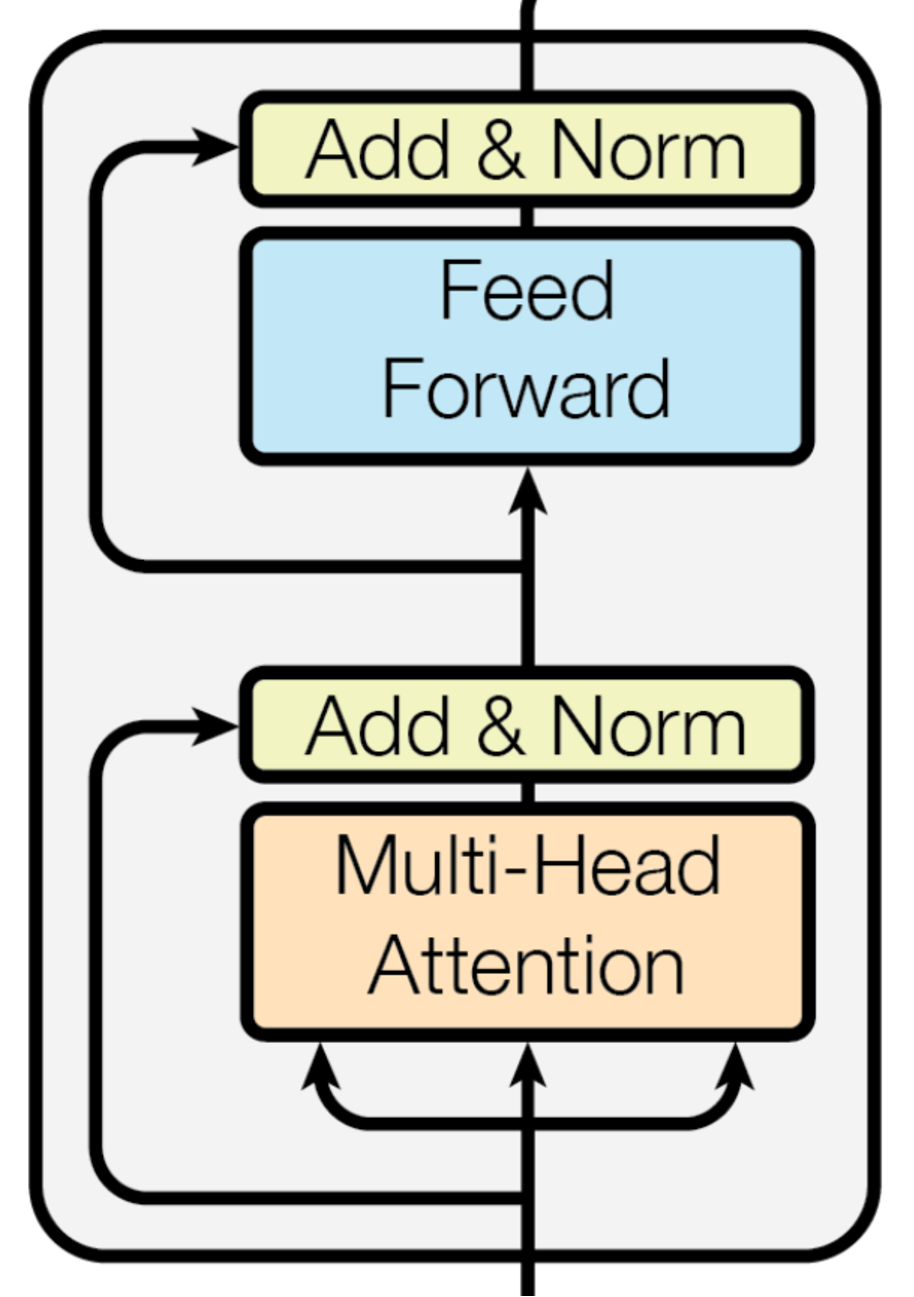
\includegraphics[width=0.23\textwidth]{img/transformer/encoder}
  }
  \quad
  \subfloat[Decoder\label{fig:transformer:decoder}]{%
    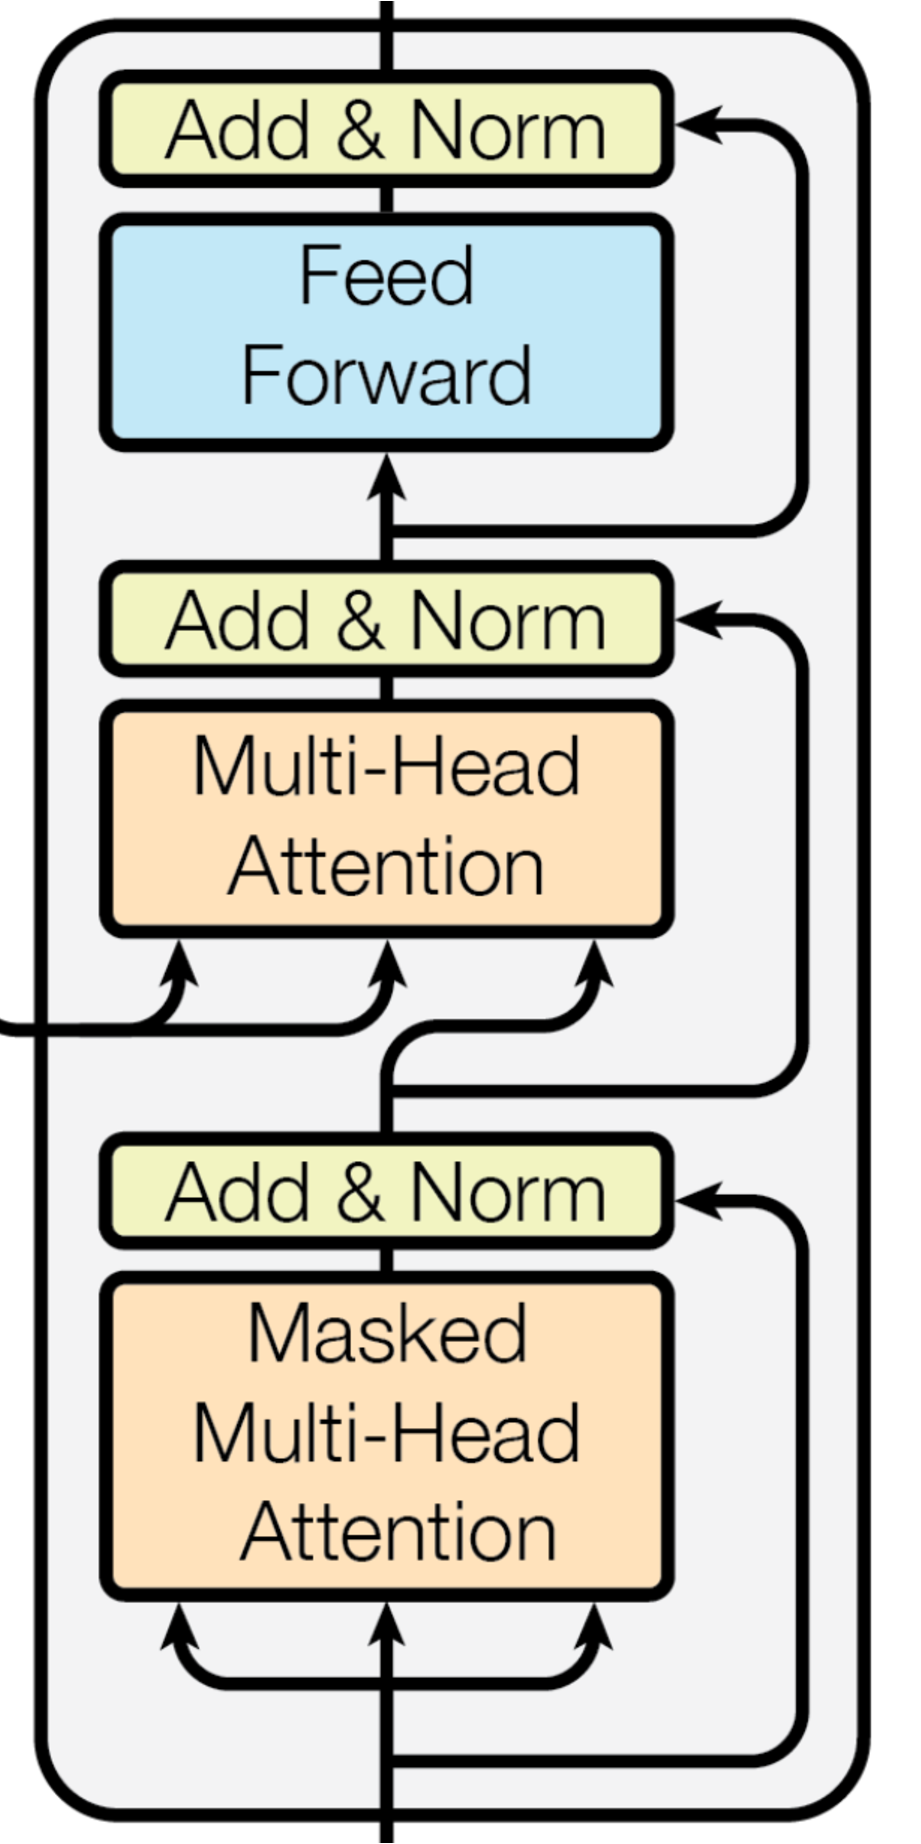
\includegraphics[width=0.23\textwidth]{img/transformer/decoder}
  }
  \caption{One Layer of the Architecture of the Transformer.}
  \label{fig:transformer:architecture:encoder}
  \source{\textsc{Vaswani} et al. -- Attention Is All You Need.}
\end{figure}

In Figure \ref{fig:transformer:encoder}, one layer of the encoder contains two
sub-layers: a MHA mechanism and a position-wise fully connected Feed-Forward
Neural Network (FFN).
\begin{definition}[Feed-Forward Neural Network]
  Let $W_1 + b_1$ and $W_2 + b_2$ be two linear transformations. Mathematically,
  the FFN is defined as follows:
  \begin{equation}
    \mathrm{FFN}(x) = \max\left(0, xW_1 + b_1\right)W_2 + b_2
    \label{eq:def:ffn}
  \end{equation}
  where a ReLU activation function is used.
  \label{def:ffn}
\end{definition}

Moreover, a residual connection followed by a normalization of the layers wraps
each of the two sublayers. Mathematically, the output of every sub-layer is
defined as follows:
\begin{equation}
  \mathrm{LayerNorm}(x + \mathrm{Sublayer}(x))
  \label{eq:output:sub-layer}
\end{equation}
where $\mathrm{Sublayer}(x)$ refers to the implemented function by the sub-layer
itself. \\


\noindent In Figure \ref{fig:transformer:decoder}, the decoder has layers that
differ from the encoder with two sub-layer changes. The first sublayer change is
defined using \emph{Masked MHA} as the first sub-layer to prevent positions from
attending subsequent positions. The last change is adding a new sub-layer,
called \emph{Encoder-Decoder Attention} which performs MHA over the Attention
vectors of the decoder and those of the encoder. The use of this sub-layer makes
it possible to determine the different relationships between these
vectors. Finally, the generated embeddings are sent to a position-wise fully
connected FFN. Like the encoder, each sub-layer is wrapped by a residual
connection followed by a layer normalization.

From then one, the complete architecture of the Transformer is illustrated as follows:
\begin{figure}[!ht]
  \centering
  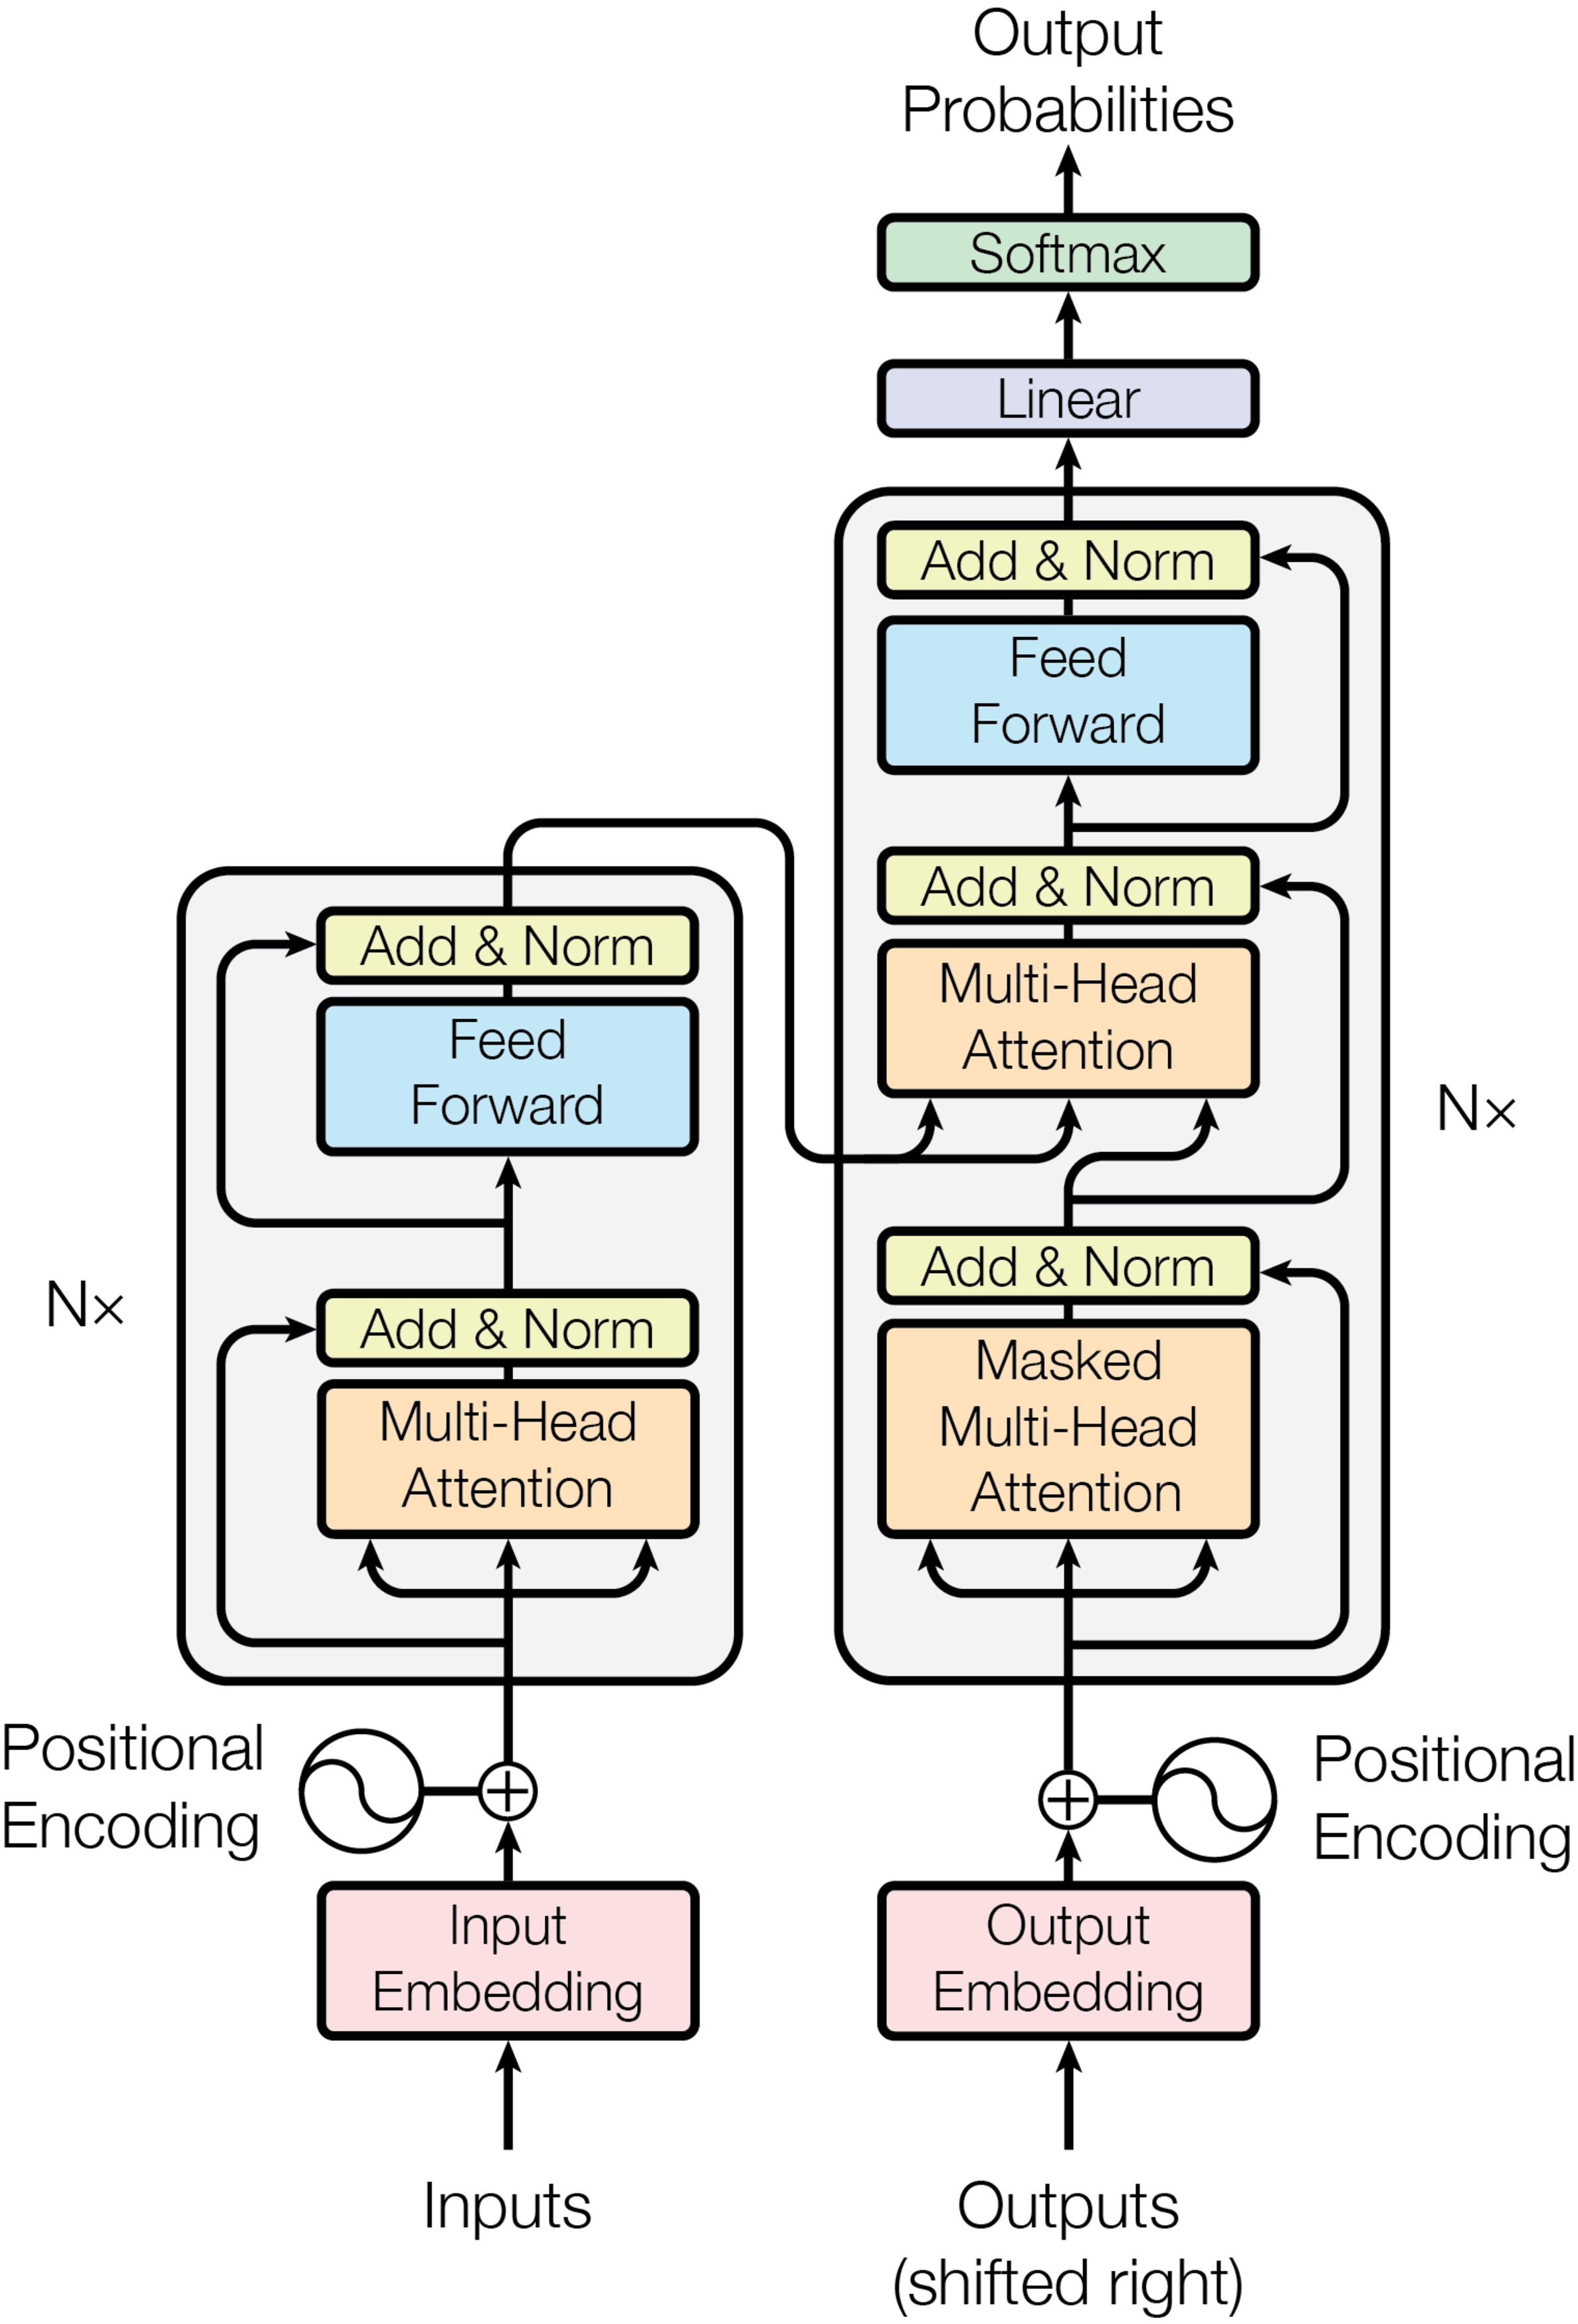
\includegraphics[width=0.6\textwidth]{img/transformer/architecture}
  \caption{Model Architecture of the Transformer.}
  \source{\textsc{Vaswani} et al. -- Attention Is All You Need}
  \label{fig:transformer:architecture}
\end{figure}

\newpage

In Figure \ref{fig:transformer:architecture}, both encoding and decoding take
the sum of the input/output embeddings with positional embedding as
input. Unlike RNNs, Transformer do not have a time step so that input sequences
can be injected simultaneously and converted into input embeddings. Each token
is represented in the embedding space through these input embeddings where
semantically similar tokens are closer than others. However, the decoder has the
particularity of having its input shifted. This shift avoids that a model only
learns to copy the decoder input by allowing a model to predict the target
word/character for position $i$ according to the previous one from 1 to $i-1$.

At last, the output of the decoding layer is sent to a linear layer. This layer
is nothing more than an FFN layer whose objective is to extend the dimension of
this vector to the number of words of the language concerned. Once expanded,
this vector is submitted to a softmax activation function to transform it into a
probability distribution and predict the next word according to the word with
the highest probability. Afterward, this decoding process is iterated several
times until the end-of-sentence token is generated.

\subsection{Positional Encoding}
\label{subsec:transformer:positional:encoding}

Considering that the transformer has no recurrence or convolution mechanism, the
architecture cannot know the order in an input sequence. From then on, the
transformer encodes the same meaning for different sentences. The easiest way to
take this context into account is to encode these positions as one-hot features.
\begin{definition}[Positional Encoding as One-Hot Features]
  Let $x \in \mathbb{R}^{n \times d}$ be a matrice of sequentially ordered data
  along the $n$-dimensional axis, and $e_k$ be a $k$'th standard basis vector in
  $\mathbb{R}^n$. Mathematically, the $z \in \mathbb{R}^{n \times d}$ learned
  combined representation is defined as follows:
  \begin{equation}
    \mathrm{z}_k = W^T_zReLU\left(W_x^Tx_k + W_e^Te_k\right), W_x \in
    \mathbb{R}^{dim(x)\times m}, W_e \in \mathbb{R}^{n\times m}, W_z \in \mathbb{R}^{m\times d}
    \label{eq:def:positional:encoding:one:hot}
  \end{equation}
  \label{def:positional:encoding:one:hot}
\end{definition}

\noindent Another approach for positional encoding is to build distinct
representations of inputs and positions~\citep{gehring}. Despite these existing
approaches to differentiate meanings, the original Transformer paper uses a
sinusoid-wave-based positional encoding to inject absolute positional
information of tokens into the sequence.

\begin{definition}[Positional Encoding by \textsc{Vaswani} et al.]
  Let $d_{model}$ be the embedding dimension of words, and $pos \in \left[0, L -
    1\right]$ be the position of a $w$ word in the $w = (w_0,\dotsc,w_{L-1})$ input
  sequence. Mathematically, the positional encoding of $w$ is defined as follows:
  \begin{align}
    \mathrm{PE}(pos,i) = \begin{cases}
      \sin\displaystyle\left(\frac{pos}{10000^{2i/d_{model}}}\right)\,, & i = 2k \\\\
      \cos\displaystyle{\left(\frac{pos}{10000^{2i/d_{model}}}\right)}\,, & i = 2k + 1
    \end{cases} \   k \in \mathbb{N}
    \label{eq:positional:encoding}
  \end{align}

  where the positional encoding follows a specific, learned pattern to identify
  word position or the distance between words in the sequence~\citep{alammar}.  In
  Equation \ref{eq:positional:encoding}, the sinusoidal representation works as
  well as a learned representation and better generalizes sequences that are
  longer than the training sequences~\citep{vaswani:attention}.
\end{definition}

%%% Local Variables:
%%% mode: latex
%%% TeX-master: "../../report"
%%% End:


%%% Local Variables:
%%% mode: latex
%%% TeX-master: "../report"
%%% End:


\chapter{Embedding Techniques}
\label{chap:embedding:techniques}

This chapter explains the Word2Vec, FastText, and Bidirectional Encoder
Representations from Transformers (BERT) embedding techniques.


\section{Word2Vec}
\label{sec:w2v}

Word2Vec is an unsupervised learning algorithm published in 2013, which, based
on a corpus of text, provides a vector representation for each word of that
text, using a two-layer neural network. This algorithm was initially implemented
to learn word representations from large data sets efficiently but emerged as a
standard embedding technique. According to the use case, two models are
available: Continuous Bag-Of-Words (CBOW) and Skip-Gram (SG).

\subsection{Continuous Bag-of-Words Model}
\label{subsec:w2v:cbow}

CBOW is an unsupervised model that predicts a target word based on context words
and window size. From a semantic point of view, the model is named
``Bag-of-Words'' since the order of the context words does not influence its
training.
\begin{figure}[!ht]
  \centering
  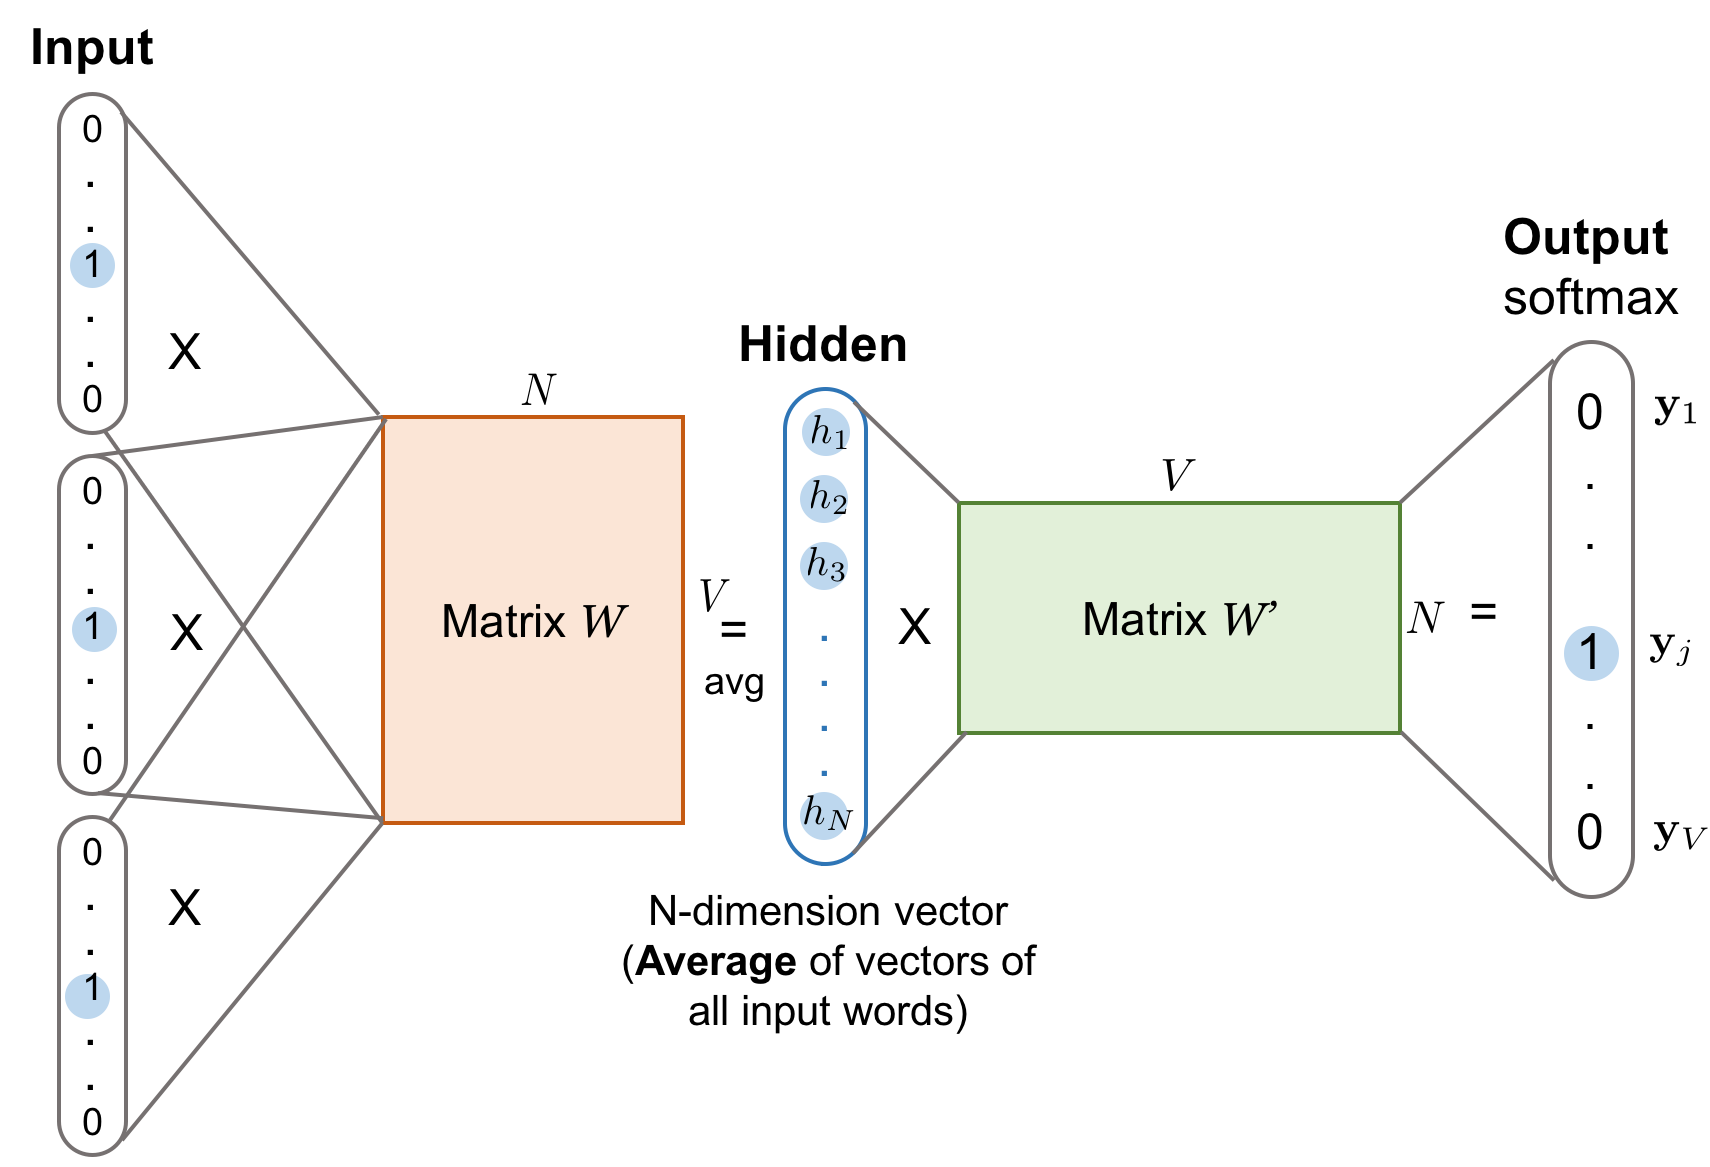
\includegraphics[width=0.75\textwidth]{img/embedders/w2v/cbow}
  \caption{CBOW Model Architecture.}
  \source{
    \href{https://lilianweng.github.io/lil-log/2017/10/15/learning-word-embedding.html}
    {Lilian Weng -- Learning Word Embedding}
  }
  \label{fig:w2v:cbow:architecture}
\end{figure}

In Figure \ref{fig:w2v:cbow:architecture}, the CBOW model architecture starts by
taking one or several targets word as input, represented as a $V$-dimensional
one-hot encoding vector. $V$ is the dictionary's size of unique words present in
a text or in a training data set. Using a dot product, this/these input
vector(s) is then multiplied by a first $W$ weight matrix, named embedding
matrix. This matrix is of dimension $V \times N$, where $N$ is the number of
features that each unique word in this vocabulary has defining the
\emph{embedding size}. Therefore, these dot products produce an $N$-dimensional
hidden vector for each input vector. However, if there multiple input context
vectors, these hidden vectors are then averaged element-wise into a single
hidden vector, where this vector chooses the size of the vectors that will be
used later.

According to the semantics of the words of the dictionary, a new dot product is
made, but this time, between the calculated hidden vector and another $W'$
weight matrix, named \emph{context matrix}. This matrix being now of dimension
$N \times V$. Then, their product generates an output vector of dimension $V$
subjected to a softmax activation function. Therefore, this function ends by
calculating a probability distribution and returns the probability that a word
is a target word for the given context words. Finally, a cross-entropy loss
function is applied to compute the loss between the true probability
distribution of the given target word and the calculated model probability.

\begin{definition}[Cross-Entropy]
  Measures the difference between two probability distributions for a given
  random variable. Let $p$ be a true probability distribution, $q$ be a computed
  model probability, and $c$ be the predicted result by an ML
  algorithm. Mathematically, the cross-entropy loss can be defined as follows:
  \begin{equation}
    H(p, q) = -\sum_{c=1}^Cp(c)\log\left(q(c)\right)
    \label{eq:cross-entropy}
  \end{equation}
  \label{def:cross-entropy}
\end{definition}

After computation with the cross-entropy loss, the back-propagation updates the
weights of the embedding matrix according to this loss. These steps are then
repeated with other context words and another target word for a specified number
of epochs. Once the training is done, the embedding matrix is used to generate
the word embeddings from the one-hot encodings. Formally, given a sequence of
training words $w_1, w_2, \dotsc, w_t$, and a context window $c$, the objective
of the CBOW model is to maximize the average log probability:
\begin{equation}
  \frac{1}{T}\sum_{t=1}^T\log\left(p\left(w_t|w_{t-c}, \ldots, w_{t + c}\right)\right)
  \label{eq:w2v:cbow:probability}
\end{equation}

where $T$ is the number of training samples, and the probability
$p\left(w_t|w_{t-c}, \ldots, w_{t + c}\right)$ is computed using the softmax
function (cf. Definition \ref{def:softmax}):
\begin{equation}
  p\left(w_t|w_{t-c}, \ldots, w_{t + c}\right) =
  \frac{\exp\left(v^{-T}v'_{w_t}\right)}{\sum_{w=1}^W\exp\left(v^{-T}v'_w\right)}
  \label{eq:w2v:cbow:probability:details}
\end{equation}

where $W$ is the vocabulary size, $v'_w$ is the output vector of the $w$ word,
and $v$ is the averaged input vector of all the context words:
\begin{equation}
  \overline{w}_t = \frac{1}{2c}\sum_{-c\leq j \leq c,j \neq 0}w_{t + j}
  \label{eq:w2v:cbow:probability:details2}
\end{equation}

\noindent Finally, the whole network is not used regarding the generation of embeddings,
but only its first layer.

\subsection{Skip-Gram Model}
\label{subsec:w2v:sg}

SG is an unsupervised model that predicts context words from a target word,
according to window size and a sentence. Unlike CBOW, these context words are
defined as multiple pairs of words (cf. Table \ref{def:window:size}), serving as
training samples for this model. Such training allows this model to learn word
vector representations suitable for predicting nearby words within a text,
except for common words and stop words (cf. Section
\ref{subsec:w2v:sfw}). Finally, SG compresses the information in a low
dimensional space, such that this model learns a continuous low dimensional
representation for the words.

The window size for each target word is arbitrarily chosen between one and a
small positive number. This choice allows to add randomness during training and
improves future predictions. In the case of a window size greater than two, the
context words for a target word likely are more than two. If such a situation
occurs, SG randomly picks a word from these word contexts to form a pair with
the context word. Then, this model counts the number of times this pair of words
appear, and the model starts to be trained.

Similar to CBOW, given a sequence of target words $w_1, w_2, \ldots, w_t$, and a
context window $c$, the objective of the SG model is to maximize the average log
probability:
\begin{equation}
  \frac{1}{T}\sum_{t=1}^T\sum_{-c \leq j \leq c, j \neq 0}\log\left(p\left(w_{t+j}|w_t\right)\right)
  \label{eq:w2v:sg:probability}
\end{equation}

where $T$ is the number of training samples, and the probability $p\left(w_{t +
j}|w_t\right)$ is also computed using the softmax function (cf. Definition
\ref{def:softmax}):
\begin{equation}
  p\left(w_o|w_i\right) = \frac{\exp\left(u_{w_o}^Tv_{w_i}\right)}{\sum_{w=1}^W\exp\left(u_w^Tv_{w_i}\right)}
  \label{eq:w2v:sg:probability:details}
\end{equation}
where $W$ is the vocabulary size, $v$ the input representation of a word, and
$u$ the output representation of a word.

\begin{figure}[!ht]
  \centering
  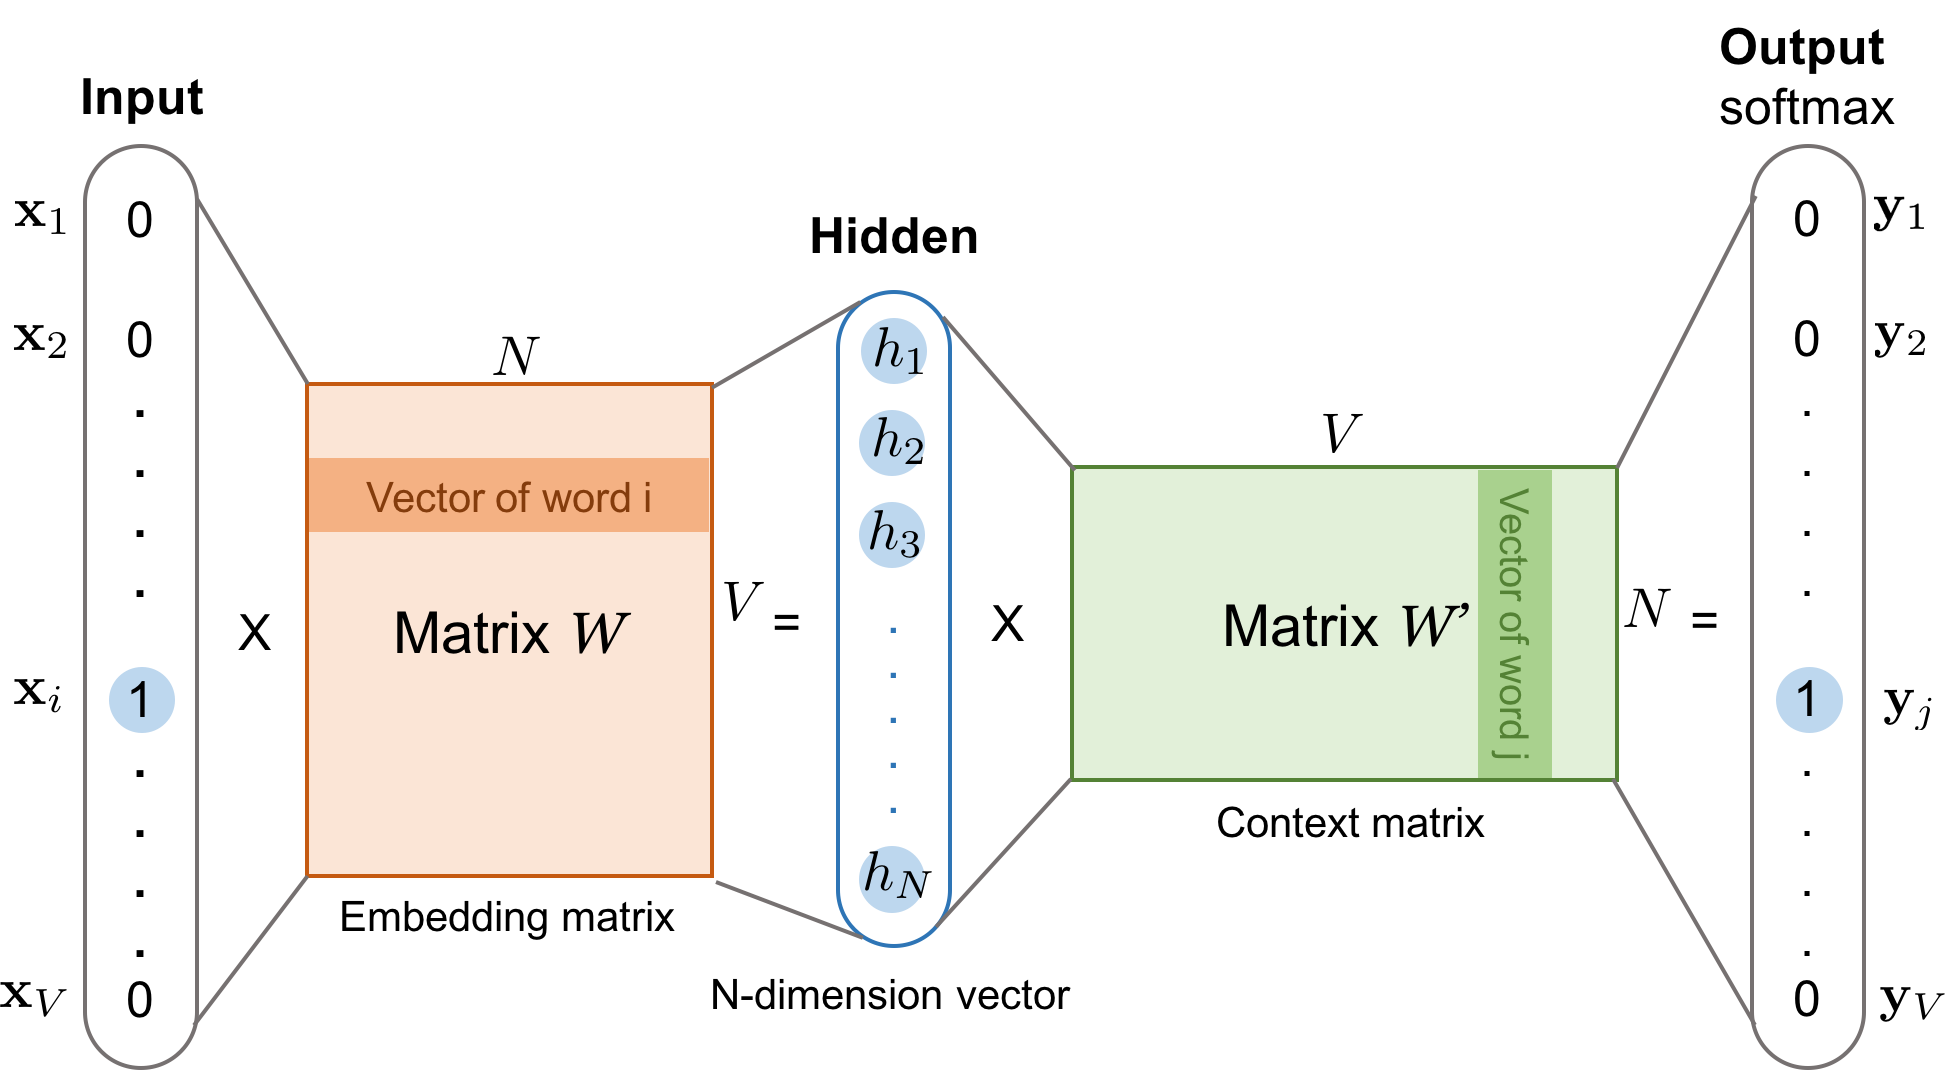
\includegraphics[width=0.8\textwidth]{img/embedders/w2v/skip-gram}
  \caption{SG Model Architecture.}
  \source{
    \href{https://lilianweng.github.io/lil-log/2017/10/15/learning-word-embedding.html}
    {Lilian Weng -- Learning Word Embedding}
  }
  \label{fig:w2v:sg:architecture}
\end{figure}

In Figure \ref{fig:w2v:sg:architecture}, the SG model architecture can be seen
as the inverse of the CBOW architecture. With this architecture, instead of
having context words and predicting a target word, it takes two words. From then
on, a model will predict a target word according to a context word. In addition,
since there is only one input word, the embedding matrix directly generates a
hidden layer with no need to do an average. Finally, the cross-entropy loss
function is applied this time to compute the loss between the true probability
distribution of the given context word and the calculated model probability.

\subsection{Subsampling Frequent Words}
\label{subsec:w2v:sfw}

Subsampling frequent words is a technique whose objective is to reduce the
number of training examples for a Word2Vec model. To accomplish this, it assumes
that predicting context words that are too frequent (e.g., ``the'') provides
little semantic value to differentiate a context
~\citep{inproceedings:mikolov}. In contrast, infrequent words are more likely to
convey specific information. Therefore, to improve the balance between
infrequent and frequents words, this technique randomly eliminates words from a
more frequent corpus than a certain threshold. This suppression occurs before a
corpus is processed in word-context pairs.

Let $w_i$ be a word, $f_{w_i}$ be a word frequency in a corpus, and $t$ be a
chosen threshold, typically around $10^{-5}$. Mathematically, the discarding of
a word from a corpus is done as follows:
\begin{equation}
  P(w_i) = 1 - \sqrt{\frac{t}{f(w_i)}}
  \label{eq:w2v:sfw}
\end{equation}

Therefore, each word $w_i$ present in a text for a window of size $c$ has a
probability of being deleted, where each deleted word reduces the training
samples by most $c$ times. Therefore, words whose frequency is above this
threshold, will be aggressively subsampled, preserving the frequency
ranking. However, even though this formula speeds up learning and even
significantly improves the accuracy of learned vectors of infrequent
words~\citep{inproceedings:mikolov}, the Word2Vec implementation uses another
more elaborate formula to discard a word:
\begin{equation}
  P(w_i) = \left(\sqrt{\frac{z(w_i)}{t}} + 1\right)\frac{t}{z(w_i)}
  \label{eq:w2v:sfw:real}
\end{equation}

where $t$ has a default threshold of $10^{-3}$ and $z(w_i)$ is the fraction of
the total words in the corpus that corresponds to this word. For example, if the
``cat'' word occurs 1000 times in a billion words corpus, then $z($``cat''$) =
10^{-6}$. Therefore, $P(w_i) = 1$ when $z(w_i) \leq 0.0032z(w_i) \leq 0.0032$
means to keep every instance of a word that represented \SI{0.32}{\percent} or
less and subsampled those that have a higher percentage. Please note that
$P(w_i)$ does not correspond to a probability since it is no longer bounded
between 0 and 1. Finally, from the accuracy point of view, subsampling frequent
words can improve some accuracy and decrease one of the others.

\subsection{Hierarchical Softmax}
\label{subsec:w2v:hsm}

Hierarchical Softmax (HSM) is an efficient softmax approximation technique that
uses a multilayer binary tree structure to reduce the computational cost of
training a softmax neural network~\citep{DBLP:conf/aistats/MorinB05}. In this
data structure, each node without child nodes, called \emph{leaf nodes},
corresponds to a word and each internal node stands for relative probabilities
of the children nodes.

For better accuracy, HSM structures the Word2Vec vocabulary using a
\textsc{Huffman} tree, a binary tree data structure where data is stored in leaf
nodes, without any particular order. To structure this vocabulary, HSM uses this
tree so that frequent words are closer to the root node of the tree while
infrequent words are deeper in this tree. Therefore, more frequent words have a
greater weight than infrequent words, where the \emph{path length} is
proportional to the frequency of a word. The path length of a tree is defined as
the number of nodes that must be traversed to reach a specific
word. Consequently, a \textsc{Huffman} tree always has $n$ leaf nodes for $n-1$
internal nodes, where each node is characterized by a weight defined by a
numerical identifier. As a result, the weight of each parent node is equal to
the sum of the lower weights of its children.

To compute the probability distribution of reaching a word, HSM uses a sigmoid
activation function and two matrices. One for the inputs and one for the outputs
differ on the values stored in each row.
\begin{table}[!ht]
  \centering
  \begin{subtable}[b]{0.5\textwidth}
    \centering
    \begin{tabular}{cc}
      \toprule
      \textbf{Target Word} & \textbf{Context Words} \\
      \midrule
      \dots & \dots, \dots \\
      sleep & sleep, cat \\
      \bottomrule
    \end{tabular}
    \caption{Input Matrix}
  \end{subtable}%
  \begin{subtable}[b]{0.5\textwidth}
    \centering
    \begin{tabular}{ccc}
      \toprule
      \textbf{Node} & \textbf{Sigmoid Value} &  \textbf{Label} \\
      \midrule
      \dots & \dots & \dots \\
      14 & 0.84 & 1 \\
      20 & 0.23 & 0 \\
      \bottomrule
    \end{tabular}
    \caption{Output Matrix}
  \end{subtable}
  \caption{HSM Matrices for the SG Model.}
  \label{fig:w2v:hsm:matrices}
\end{table}

In Table \ref{fig:w2v:hsm:matrices}, the input matrix of a SG model contains
training samples for different target words. On the other hand, the output
matrix has rows of node weights related to labels and a probability determined
by the sigmoid function. This label, which can only have two values (zero or
one), helps informs navigation in the tree based on a node. By convention, zero
means to browse the left branch of this tree and one, the other
branch. Therefore, the output matrix reports that the ``cat'' context word is
found for the ``sleep'' target word by turning left at node 20 and turning right
at node 14.

\begin{figure}[!ht]
  \centering
  \resizebox{0.6\textwidth}{!}{%
    \begin{tikzpicture}
      \node[entity,minimum size=0.9cm,fill=myblue] (node_20) at (0,0) {20};

      \node[entity,minimum size=0.9cm,fill=myblue] (node_14) at (-2.5,-1) {14};
      \node[entity,minimum size=0.9cm,fill=myblue] (node_6) at (2.5,-1) {6};

      \node[entity,minimum size=0.9cm,fill=myblue] (node_dog) at (-4,-2.5) {8};
      \node[circle,draw,fill=myred] (node_cat) at (-1,-2.5) {9};

      \node[entity,minimum size=0.9cm,fill=myblue] (node_rabbit) at (1,-2.5) {4};
      \node[entity,minimum size=0.9cm,fill=myblue] (node_2) at (4,-2.5) {2};

      \node[entity,minimum size=0.9cm,fill=myblue] (node_horse) at (2.5,-4) {1};
      \node[entity,minimum size=0.9cm,fill=myblue] (node_fish) at (5.5,-4) {1};

      \draw[color=red,text=black] (node_20) -- (node_14) node[edge] {\textcolor{red}{0}};
      \draw (node_20) -- (node_6) node[edge] {1};

      \draw[color=red,text=black] (node_14) -- (node_cat) node[edge] {\textcolor{red}{1}};
      \draw (node_14) -- (node_dog) node[edge] {0};

      \draw (node_6) -- (node_rabbit) node[edge] {0};
      \draw (node_6) -- (node_2) node[edge] {1};

      \draw (node_2) -- (node_horse) node[edge] {0};
      \draw (node_2) -- (node_fish) node[edge] {1};

      \node[label,below of=node_cat] {\textcolor{red}{\textbf{cat}}};
      \node[label,below of=node_dog] {dog};
      \node[label,below of=node_rabbit] {rabbit};
      \node[label,below of=node_horse] {horse};
      \node[label,below of=node_fish] {fish};
    \end{tikzpicture}
    }%
  \caption{\textsc{Huffman} Tree for Word2Vec.}
  \label{fig:w2v:hsm:huffman}
\end{figure}

In Figure \ref{fig:w2v:hsm:huffman}, a vocabulary of five words is structured in a
\textsc{Huffman} tree containing four internal nodes, where each edge indicates a
label. This training aims to teach the model to navigate in the tree by finding
a context word based on a target word. For this search, the tree is traversed
from top to bottom, where HSM does the dot product between the target word
vector and the current node. Afterward, the result is sent to a sigmoid
activation function which returns a probability value. According to this value,
HSM checks that this probability is correct based on a label and updates the
neurons' weights if needed. This process is repeated until the word context for
a target word is found. Since training is not done on all words, there is no
need to traverse every tree node. As a result, the complexity of the gradient
goes from $\mathcal{O}(W)$ to $\mathcal{O}(\log_2(w))$. Once the training is
completed, the SG model (the same reasoning is used for CBOW) can use this tree
to predict a context word for a target word, where this time the label is not
specified in the output matrix.

\begin{figure}[!ht]
  \centering
    \resizebox{0.6\textwidth}{!}{%
    \begin{tikzpicture}
      \node[entity,minimum size=0.9cm,fill=myblue] (node_20) at (0,0) {20};

      \node[entity,minimum size=0.9cm,fill=myblue] (node_14) at (-2.5,-1) {14};
      \node[entity,minimum size=0.9cm,fill=myblue] (node_6) at (2.5,-1) {6};

      \node[entity,minimum size=0.9cm,fill=myblue] (node_dog) at (-4,-2.5) {8};
      \node[entity,minimum size=0.9cm,fill=myblue] (node_cat) at (-1,-2.5) {9};

      \node[entity,minimum size=0.9cm,fill=myred] (node_rabbit) at (1,-2.5) {4};
      \node[entity,minimum size=0.9cm,fill=myblue] (node_2) at (4,-2.5) {2};

      \node[entity,minimum size=0.9cm,fill=myblue] (node_horse) at (2.5,-4) {1};
      \node[entity,minimum size=0.9cm,fill=myblue] (node_fish) at (5.5,-4) {1};

      \draw (node_20) -- (node_14) node[edge] {0.73};
      \draw[color=red,text=black] (node_20) -- (node_6) node[edge] {\textcolor{red}{0.27}};

      \draw (node_14) -- (node_cat) node[edge] {0.55};
      \draw (node_14) -- (node_dog) node[edge] {0.45};

      \draw[color=red,text=black] (node_6) -- (node_rabbit) node[edge] {\textcolor{red}{0.62}};
      \draw (node_6) -- (node_2) node[edge] {0.38};

      \draw (node_2) -- (node_horse) node[edge] {0.81};
      \draw (node_2) -- (node_fish) node[edge] {0.19};

      \node[label,below of=node_cat] {cat};
      \node[label,below of=node_dog] {dog};
      \node[label,below of=node_rabbit] {\textcolor{red}{\textbf{rabbit}}};
      \node[label,below of=node_horse] {horse};
      \node[label,below of=node_fish] {fish};
    \end{tikzpicture}
    }%
    \caption{\textsc{Huffman} Tree for Word2Vec.}
  \label{fig:w2v:hsm:huffman:prediction}
\end{figure}

In Figure \ref{fig:w2v:hsm:huffman:prediction}, the tree edges provide the
number of occurrences that a context word is to the left or right of a node,
according to a given target word. After training this SG model for training
data, the output matrix indicates that \SI{27}{\percent} of the time, the
context word for the same target word was in the right branch of the root node,
and \SI{73}{\percent} of the time, this context word was left branch. Based on
this principle, the other nodes also return a probability distribution for their
left and right branches that varies according to the input vector of a target
word.

Therefore, the probability of having ``rabbit'' as a context word for the
``sleep'' target word is equal to the product of the probabilities ($\simeq$
\SI{17}{\percent}). Added to the probability distribution, each word in the
vocabulary guarantees that its sum is unitary. Finally, through HSM, Word2Vec
can retrieve word input vectors where the probability distribution of two
synonymous words will have a cosine similarity close to one.

\subsection{Negative Sampling}
\label{subsec:w2v:ns}

Negative sampling is an alternative technique to HSM, which also reduces the
training speed but combined with Subsampling Frequent Words, it can improve the
word embeddings' quality. To achieve this, \textsc{Mikolov} et al. assume that
updating all the neurons of a ANN for each training sampling is computationally
expensive. From then on, negative sampling focuses on making each training
sample change only a tiny percentage of the weights rather than all of
them~\citep{mccormick}. However, with or without negative sampling, the hidden
layer only updates the input word weights.

The way negative sampling works can be considered a simplified version of the
Noise Contrastive Estimation (NCE) metric, whose purpose of NCE is to learn a
data distribution by comparing it against a noise distribution. In the context
of negative sampling, the latter differentiates a target word from noise samples
using a logistic regression classifier~\citep{DBLP:journals/jmlr/GutmannH10}.

The words being stored in one-hot vectors, this technique updates the weights of
the ``positive'' and ``negative'' words. A word is considered positive if it was
initially in the training sample, while a word is negative if it is considered
noise. Specifically, this noise results from the return of the zero value in
these one-hot vectors by the ANN. A small number makes selecting these negative
words of random words using a ``unigram distribution'', where the most frequent
words are more likely to be chosen as negative samples~\citep{mccormick}.

Let $w_i$ be a word from a corpus, $f_{w_i}$ be a word frequency, and $w_j$ be a
total number of negative words in the corpus. The probability that a $w_i$ word
is selected as a negative word is defined as follows:
\begin{equation} P(w_i) = \frac{f(w_i)}{\sum_{j=0}^nf(w_j)}
  \label{eq:w2v:ns:selection:intro}
\end{equation}

However, the published version increases the number of words to 3/4 power to
provide better results. The following formula also increases the probability of
infrequent words and decreases the likelihood of frequent words:
\begin{equation} P(w_i) = \frac{f(w_i)^{3/4}}{\sum_{j=0}^nf(w_j)^{3/4}}
  \label{eq:w2v:ns:selection}
\end{equation}

In practice, Word2Vec implements this negative sampling selection by filling a
table called \emph{unigram table}, including the index of each word present in a
vocabulary~\citep{mccormick}. Then, the selection of a negative sample is made
by generating a random index, where the index of a word appears $P(w_i) *
{table}_{\text{size}}$ times in a table. Therefore, the more frequent words are
more likely to be negative words. Finally, for the choice of the number of
negative words, it is recommended to take five to twenty words for small data
sets instead of large data sets where it is preferable to take two to five
words.~\citep{inproceedings:mikolov}.

\subsection{Advantages and Disadvantages}
\label{subsec:w2v:pro:cons}

In a non-exhaustive way, the advantages of the Word2Vec are:
\begin{itemize}
\item The use of unsupervised learning and can therefore work on any plain text.
\item Requires less RAM compared to other words/vectors representations.
\end{itemize}

As for its main disadvantages, they are the following:
\begin{multicols}{2}
\begin{itemize}
\item No embeddings are available for Out of Vocabulary (OOV) words. Therefore,
if Word2Vec has trained with the ``cat'' and ``fish'' words, it will not generate
the embedding of the ``catfish'' compound
\item No suffixes/prefixes meaning capture for given words in a corpus.
\columnbreak
\item Generation of low quality word embeddings for rare words.
\item Difficulty in determining the best value for the dimensionality of the
  word vectors and the window size.
\item The use of the softmax activation function is computationally expensive.
\end{itemize}
\end{multicols}

For the choice of the model, it is recommended to use SG when it is essential to
predict infrequent words with a small amount of training
data~\citep{inproceedings:mikolov}. However, CBOW is preferable for the
prediction of frequent words. Added to that, SG performs significantly on
semantic accuracy tests (e.g., ``Athens'' $\rightarrow$ ``Greece'' and ``Oslo''
$\rightarrow$ ``Norway''). At the same time, CBOW offers better results in
syntactic accuracy tests (e.g., ``apparent'' $\rightarrow$ ``apparently'' and
``rapid'' $\rightarrow$ ``rapidly'')~\citep{sijun_he}.

%%% Local Variables:
%%% mode: latex
%%% TeX-master: "../../report"
%%% End:


\section{FastText}
\label{sec:fasttext}

FastText is an extension to Word2Vec created by Facebook in 2016, based on the
decomposition of a word into character $n$-grams to improve the embeddings
obtained by an SG model. Unlike Word2Vec, which treats each word in a corpus as
an atomic entity, the decomposition made by FastText mainly solves the
embeddings creation for OOV words and parameter sharing between words of the
same radical. Finally, FastText can be used for unsupervised learning and
supervised learning with text classification for tasks such as spam filtering.

\subsection{Sub-Word Generation}
\label{subsec:fasttext:sub-word}

The generation of sub-words called $n$-grams is an integral part of the success
of FastText. Therefore, it is good to know the details of such a generation.

\begin{definition}[Sub-word Generation]
  Consists of adding angular brackets on either side of a word used as a
  delimiter and generating character $n$-grams of length $n$. In practice, picking
  this length allows extraction of $n$-grams $\geq$ 3 and $\geq
  6$~\citep{DBLP:journals/tacl/BojanowskiGJM17}. Let ``flying'' be a word. The
  following table illustrates the sub-word generation for character $n$-grams of
  length 3, 4, 5, and 6.

  \begin{table}[!ht]
    \centering
    \caption{Sub-word Generation for Character $N$-Grams of Length 3, 4, 5, and 6.}
    \label{tab:fasttext:sub-word}
    \begin{tabular}{ccl}
      \toprule
      \textbf{Word} & \textbf{Length} & \textbf{Character $n$-grams} \\
      \midrule
      \multirow{4}{*}{flying} & 3 & <fl, fly, lyi, yin, ing, ng> \\
                    & 4 & <fly, flyi, lyin, ying, ing> \\
                    & 5 & <flyi, lying, ying> \\
                    & 6 & <flyin, flying, lying> \\
      \bottomrule
    \end{tabular}
  \end{table}

  In Table \ref{tab:fasttext:sub-word}, each character $n$-grams of length $n$
  is generated by sliding a 2-characters window from the beginning of the bracket
  to its end.
  \label{def:sub-word:generation}
\end{definition}

As a result, the vector of a word corresponds to the sum of these $n$-grams of
characters. This word decomposition into character $n$-grams comes at a storage
cost since storing all the unique $n$-grams can quickly be significant. The
original paper uses a variant of the Fowler-Noll-Vo (FNV) hash function, called
\emph{FNV-1a}, to hash character sequences into integer values to reduce this
memory cost. The use of FNV is helpful for this use case since FNV was not
designed for cryptography but for the fast use of hash tables and
\emph{checksums}. The checksum results of performing a cryptographic hash
function on a piece of data, usually a file, to ensure that the data is
authentic and error-free. Moreover, it is necessary to learn a certain amount of
embeddings to hash character sequences. Specifically, this amount designates the
hash bucket's size to better distribute these character $n$-grams for sorting
and retrieval purposes. From then on, the hashing of each $n$-gram to a number
between one and $N$, reduces the vocabulary size in the counterpart of potential
\emph{collisions}. This hash collision means that several character $n-grams$
stored as a key can result in the same hash and checksum. Therefore no longer
ensure the authenticity of a value.

In some circumstances, the model size may be excessive. In this case, it is
still possible to reduce the hash size where the appropriate value is near
$20000$. However, it is also possible to reduce the size of the vectors at the
expense of smaller model accuracy.

\subsection{Training}
\label{subsec:fasttext:training}

Like Word2Vec, the training of FastText’s SG model can use HSM or Negative
sampling. To better understand its application with negative sampling, one can
take the following ``I always remember her'' sentence is taken. Let ``remember''
be the target word, using 3-grams and a window size of 3. This example predicts
the ``always'' and ``her'' context words. First of all, this model computes the
embeddings of the target word by summing the embeddings for the character
$n$-grams and the whole word itself:
\begin{align}
  \mathrm{E}_{remember} = e_{<re} + e_{rem} + \dots + e_{er>} + e_{remember}
  \label{eq:fasttext:embeddings}
\end{align}

Afterward, each context word is taken directly from their embeddings without
adding the character $n$-grams. Then, several random negative samples are selected
with a probability proportional to the square root of the unigram
frequency. From then on, a context word is related to five random negative
words. In the absence of $n$-gram embeddings, the Word2Vec model is used,
specifying a maximum $n$-gram length of zero.

After selecting samples, the dot product between the target word and the actual
context words computes the probability distribution. Unlike Word2Vec, there is
this time use of the sigmoid function instead of the softmax function. Finally,
the embeddings are updated with an SGD optimizer according to the calculated
loss to bring the actual context words closer to the target word. Afterward,
there is an incrementation in the distance of the negative samples.

This update of hyper-parameters for embeddings of $n$-grams adds a significant
amount of extra computation to the training process. Moreover, CBOW generates
the word embeddings by summing and averaging $n$-grams embeddings, which adds cost
compared to SG. However, these additional calculations benefit from a set of
embeddings containing the sub-words embeddings. From then on, they allow a
better accuracy of a model in most cases.

\subsection{Advantages and Disadvantages}
\label{subsec:fasttext:pro:cons}

In a non-exhaustive way, the advantages of the FastText:
\begin{multicols}{2}
\begin{itemize}
\item The use of unsupervised learning and supervised learning with text
classification for tasks such as spam filtering.
\item Captures the meaning of suffixes/prefixes for the words given in a corpus.
\item Generation of better word embeddings for rare words as their character
$n$-grams are shared with other more frequent words, adding more neighboring
contextual words and improving its probability of being selected.
\columnbreak
  \item Generation of word embeddings for OOV words.
\item Better semantic similarity between two words (e.g., king and kingdom) by
using extra information about the sub-words.
\item No compromise of accuracy when stopwords are present.
\item Significant improvement in model accuracy when used to perform syntactic
word analogy tasks for morphologically rich languages (e.g., French and German).
\end{itemize}
\end{multicols}

As for its main disadvantages, they are the following:
\begin{multicols}{2}
\begin{itemize}
\item Requires much more RAM than Word2Vec due to the sub-words generation for
each word.
\item Lower accuracy compared to Word2Vec when a model is used on semantic
analogy tasks.
\item FastText is \SI{50}{\percent} slower to train than the regular Skip-Gram model due
to the added overhead of $n$-grams compared to Word2Vec.
\item Difficulty in determining the best value for the $n$-grams generation.
\end{itemize}
\end{multicols}

%%% Local Variables:
%%% mode: latex
%%% TeX-master: "../../report"
%%% End:


\newpage

\section{BERT}
\label{sec:bert}

Bidirectional Encoder Representations from Transformers (BERT) is a
state-of-the-art NLP embedding technique published in 2018. BERT relies on the
encoder part of the Transformer and whose objective is to generate an
unsupervised language representation model. Unlike Word2Vec, the embeddings
generated by BERT are contextualized using bidirectional representations. In the
original paper, two pre-trained BERT models trained on the English Wikipedia
(\SI{2500}{M} words) and the Toronto BookCorpus (\SI{800}{M} words) are
available:
\begin{enumerate}
\item \textbf{BERT-Base}: 12-layer Transformer, 768-hidden, 12-heads, \SI{110}{M} parameters.
\item \textbf{BERT-Large}: 24-layer Transformer, 1024-hidden, 16-heads, \SI{340}{M} parameters.
\end{enumerate}

Since these models are pre-trained based on a corpus, their use fixes the
learning vocabulary. From then on, as Word2Vec and FastText, BERT could face the
presence of OOV words. As a result of these unknown words, BERT uses an adaptive
tokenization algorithm.

\subsection{Tokenization}
\label{subsec:tokenization}

BERT uses a WordPiece tokenization algorithm for the pre-training of a
model. This tokenization proposed in 2015 by Google takes its main advantage to
not replace unknown words with a \texttt{[UNK]} special token, which implies a
loss of information about the input sequence. As an alternative to this
conversion, WordPiece uses a segmentation method which breaks down a word into
several word pieces units prefixed by \texttt{\#\#}\footnote{Except for Chinese
characters, which are surrounded by spaces before any tokenization.} and
converted into unique identifiers. From then on, this algorithm allows BERT to
learn common sub-words and does not considers OOV and rares words. As for the
vocabulary ($\simeq$ \SI{30 000}{words}), the latter is initializing itself by
taking the individual characters of a language, and adding the most frequent
combinations\footnote{For example, ``u'', followed by ``g'', would have only
been merged if the probability of ``ug'' divided by ``u'', ``g'' would have been
greater than for any other symbol pair.} of a corpus.

\begin{table}[!ht]
  \centering
  \caption{Example of Tokenization With BERT.}
  \label{tab:bert:tokenization}
  \begin{tabular}{cccccccccc}
    & The & machine & loves & embeddings. & & & & & \\
    \texttt{[CLS]} & the & machine & loves & em & \#\#bed & \#\#ding & \#\#s & . & \texttt{[SEP]} \\
    101 & 1996 & 3698 & 7459 & 7861 & 8270 & 4667 & 2015 & 1012 & 102 \\
  \end{tabular}
\end{table}

In Table \ref{tab:bert:tokenization}, the input sequence of BERT allows
receiving either one sentence (e.g., for text classification) or two sentences
(e.g., for question answering) where each of them is limited to 512
characters. Beyond this limit, it is necessary to truncate the
sentence. Finally, WordPiece uses three main special tokens:
\begin{enumerate}
\item \texttt{[CLS]}: classification token inserted at the beginning of the
  input used for prediction.
\item \texttt{[SEP]}: separator token used to indicates the end of each sentence;
\item \texttt{[PAD]}: padding token used when batching sequences of different lengths.
\end{enumerate}

\subsection{Input Embeddings}
\label{subsec:bert:input:embeddings}

Unlike Transformer, BERT accepts one or two sentences as input sentences. From
then on, BERT encodes these inputs to use them for the model pre-training.

\newpage

\begin{figure}[!ht]
  \centering
  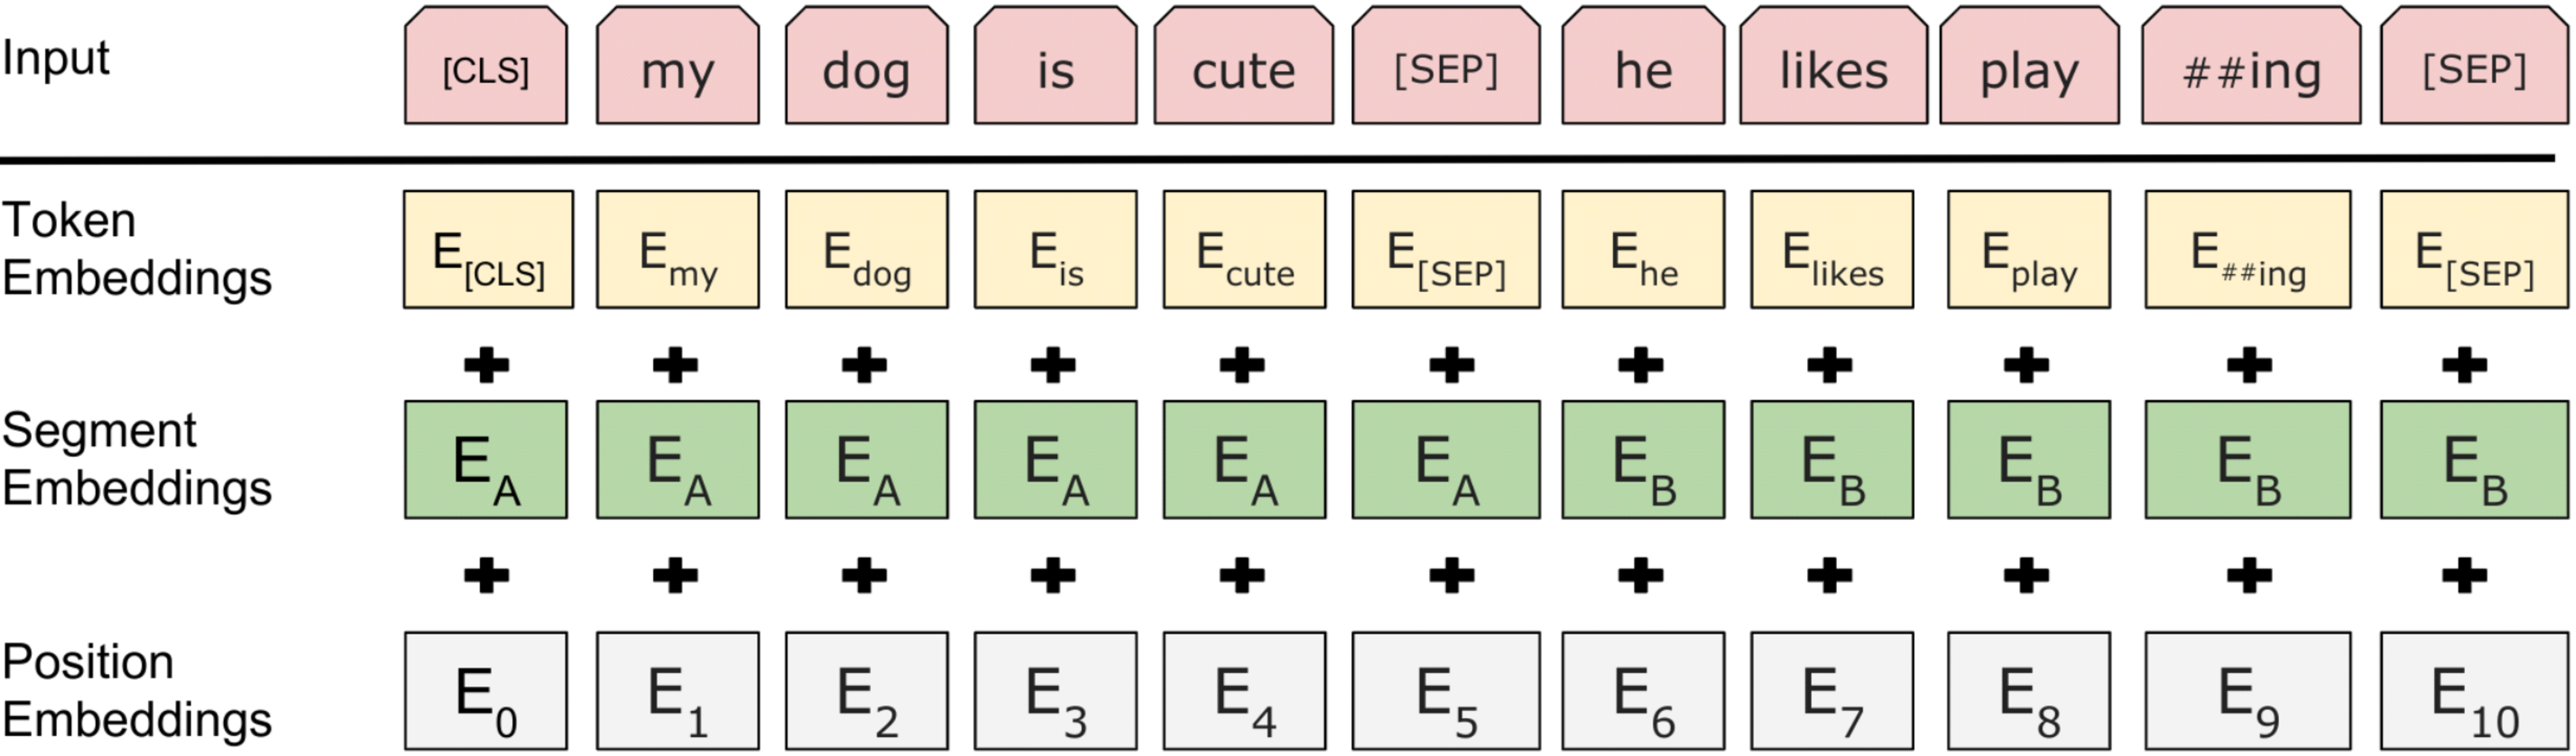
\includegraphics[width=\textwidth]{img/embedders/bert/input-embeddings}
  \caption{Example of Sentence Pair Encodding.}
  \source{\textsc{Devlin} et al. -- BERT}
  \label{fig:sentence:pair:encoding}
\end{figure}

In Figure \ref{fig:sentence:pair:encoding}, the encoding of the BERT's input
requires the sum of three vector embeddings:
\begin{enumerate}
\item \textbf{Token embeddings}: the word pieces embeddings (cf. Section
\ref{subsec:tokenization}).
\item \textbf{Segment embeddings}: the embeddings that associate a token with
its belonging sentence. In the case of a single sentence input sequence, the
vector contains only unitary values. Otherwise, the \texttt{[SEP]} token and the
tokens related to the first sentence are assigned a zero value. Those tokens of
the second sentence are assigned a unitary value.
\item \textbf{Position embeddings}: embeddings that preserve the contextual
information of the tokens by injecting their positioning into the input
embeddings, as the Transformer architecture does.
\end{enumerate}

\subsection{Pre-training}
\label{subsec:bert:pre-training}


The BERT model's pre-training gives it the ability to learn language by training
simultaneously on two unsupervised tasks: the \emph{Masked Language Model} (MLM)
and \emph{Next Sentence Prediction} (NSP). These two tasks mainly help overcome
the lack of training data and allow the model to understand better a
bidirectional representation of an input at the sentence and token level.

\subsubsection{Masked Language Model}
\label{subsubsec:bert:mlm}

MLM is the first task use by the pre-training BERT model. This task helps BERT
learn bidirectional contextual representations of tokens through the encoder
layers by predicting masked tokens from the input sequence. For this purpose,
MLM masks and predicts tokens from the input sequence. Mathematically, the
following equation defines this prediction of masked tokens.

\begin{equation}
  p\left(x_1,\dotsc,x_n\right) = \sum_{i = 1}^np\left(x_i|x_1,\dotsc,x_{i - 1}, x_{i + 1},\dotsc, x_n\right)
\label{eq:def:mlm}
\end{equation}

where each input sequence generally has \SI{15}{\percent} of its tokens hidden
according to the following subrules:
\begin{itemize}
\item a token is replaced by a \texttt{[MASK]} token in \SI{80}{\percent} of the
  cases;
\item a token is replaced randomly in \SI{10}{\percent} of the cases;
\item a token remains unchanged in \SI{10}{\percent} of the cases.
\end{itemize}

These subrules prevent the Transformer encoder from being forced to maintain a
distributive contextual representation of each input token. From then on, it is
not recommended to modify the default token masking. Too little masking would
imply a too expensive model to train, and too much masking would mean a lack of
context for a token.

\subsubsection{Next Sentence Prediction}
\label{subsubsec:bert:nsp}

The NSP is the second task use by the pre-training BERT model. This task helps
BERT learn sentence relationships by solving a binary classification problem
using Attention information shared between sentences.
\begin{table}[!ht]
  \centering
  \caption{Example of NSP With BERT.}
  \label{tab:bert:nsp}
  \begin{tabular}{lll}
    \textbf{Sentence $\mathcal{A}$} & \textbf{Sentence $\mathcal{B}$} & \textbf{Label} \\
    GNU Emacs is the best text editor. & I should use it. & \texttt{isNextSentence} \\
    GNU Emacs is the best text editor. & I have a cat. & \texttt{NotNextSentence} \\
  \end{tabular}
\end{table}

In Table \ref{tab:bert:nsp}, NSP allows the model to train itself to predict
whether sentence $\mathcal{B}$ is a continuation of sentence $\mathcal{A}$. For
this purpose, the generation of the input sequences ensures continuity of
$\mathcal{A}$ \SI{50}{\percent} of the time, labeled as \texttt{isNext}. The
rest of the time, $\mathcal{B}$ is related to a random sentence from the
provided training data set, labeled as \texttt{NotNextSentence}.

\subsubsection{Output}
\label{subsubsec:output}

Once the BERT model understands the language representation, this model is
suitable for most NLP tasks. These tasks include Neural Machine Translation,
question answering, sentiment analysis, and text summarization.
\begin{figure}[!ht]
  \centering
  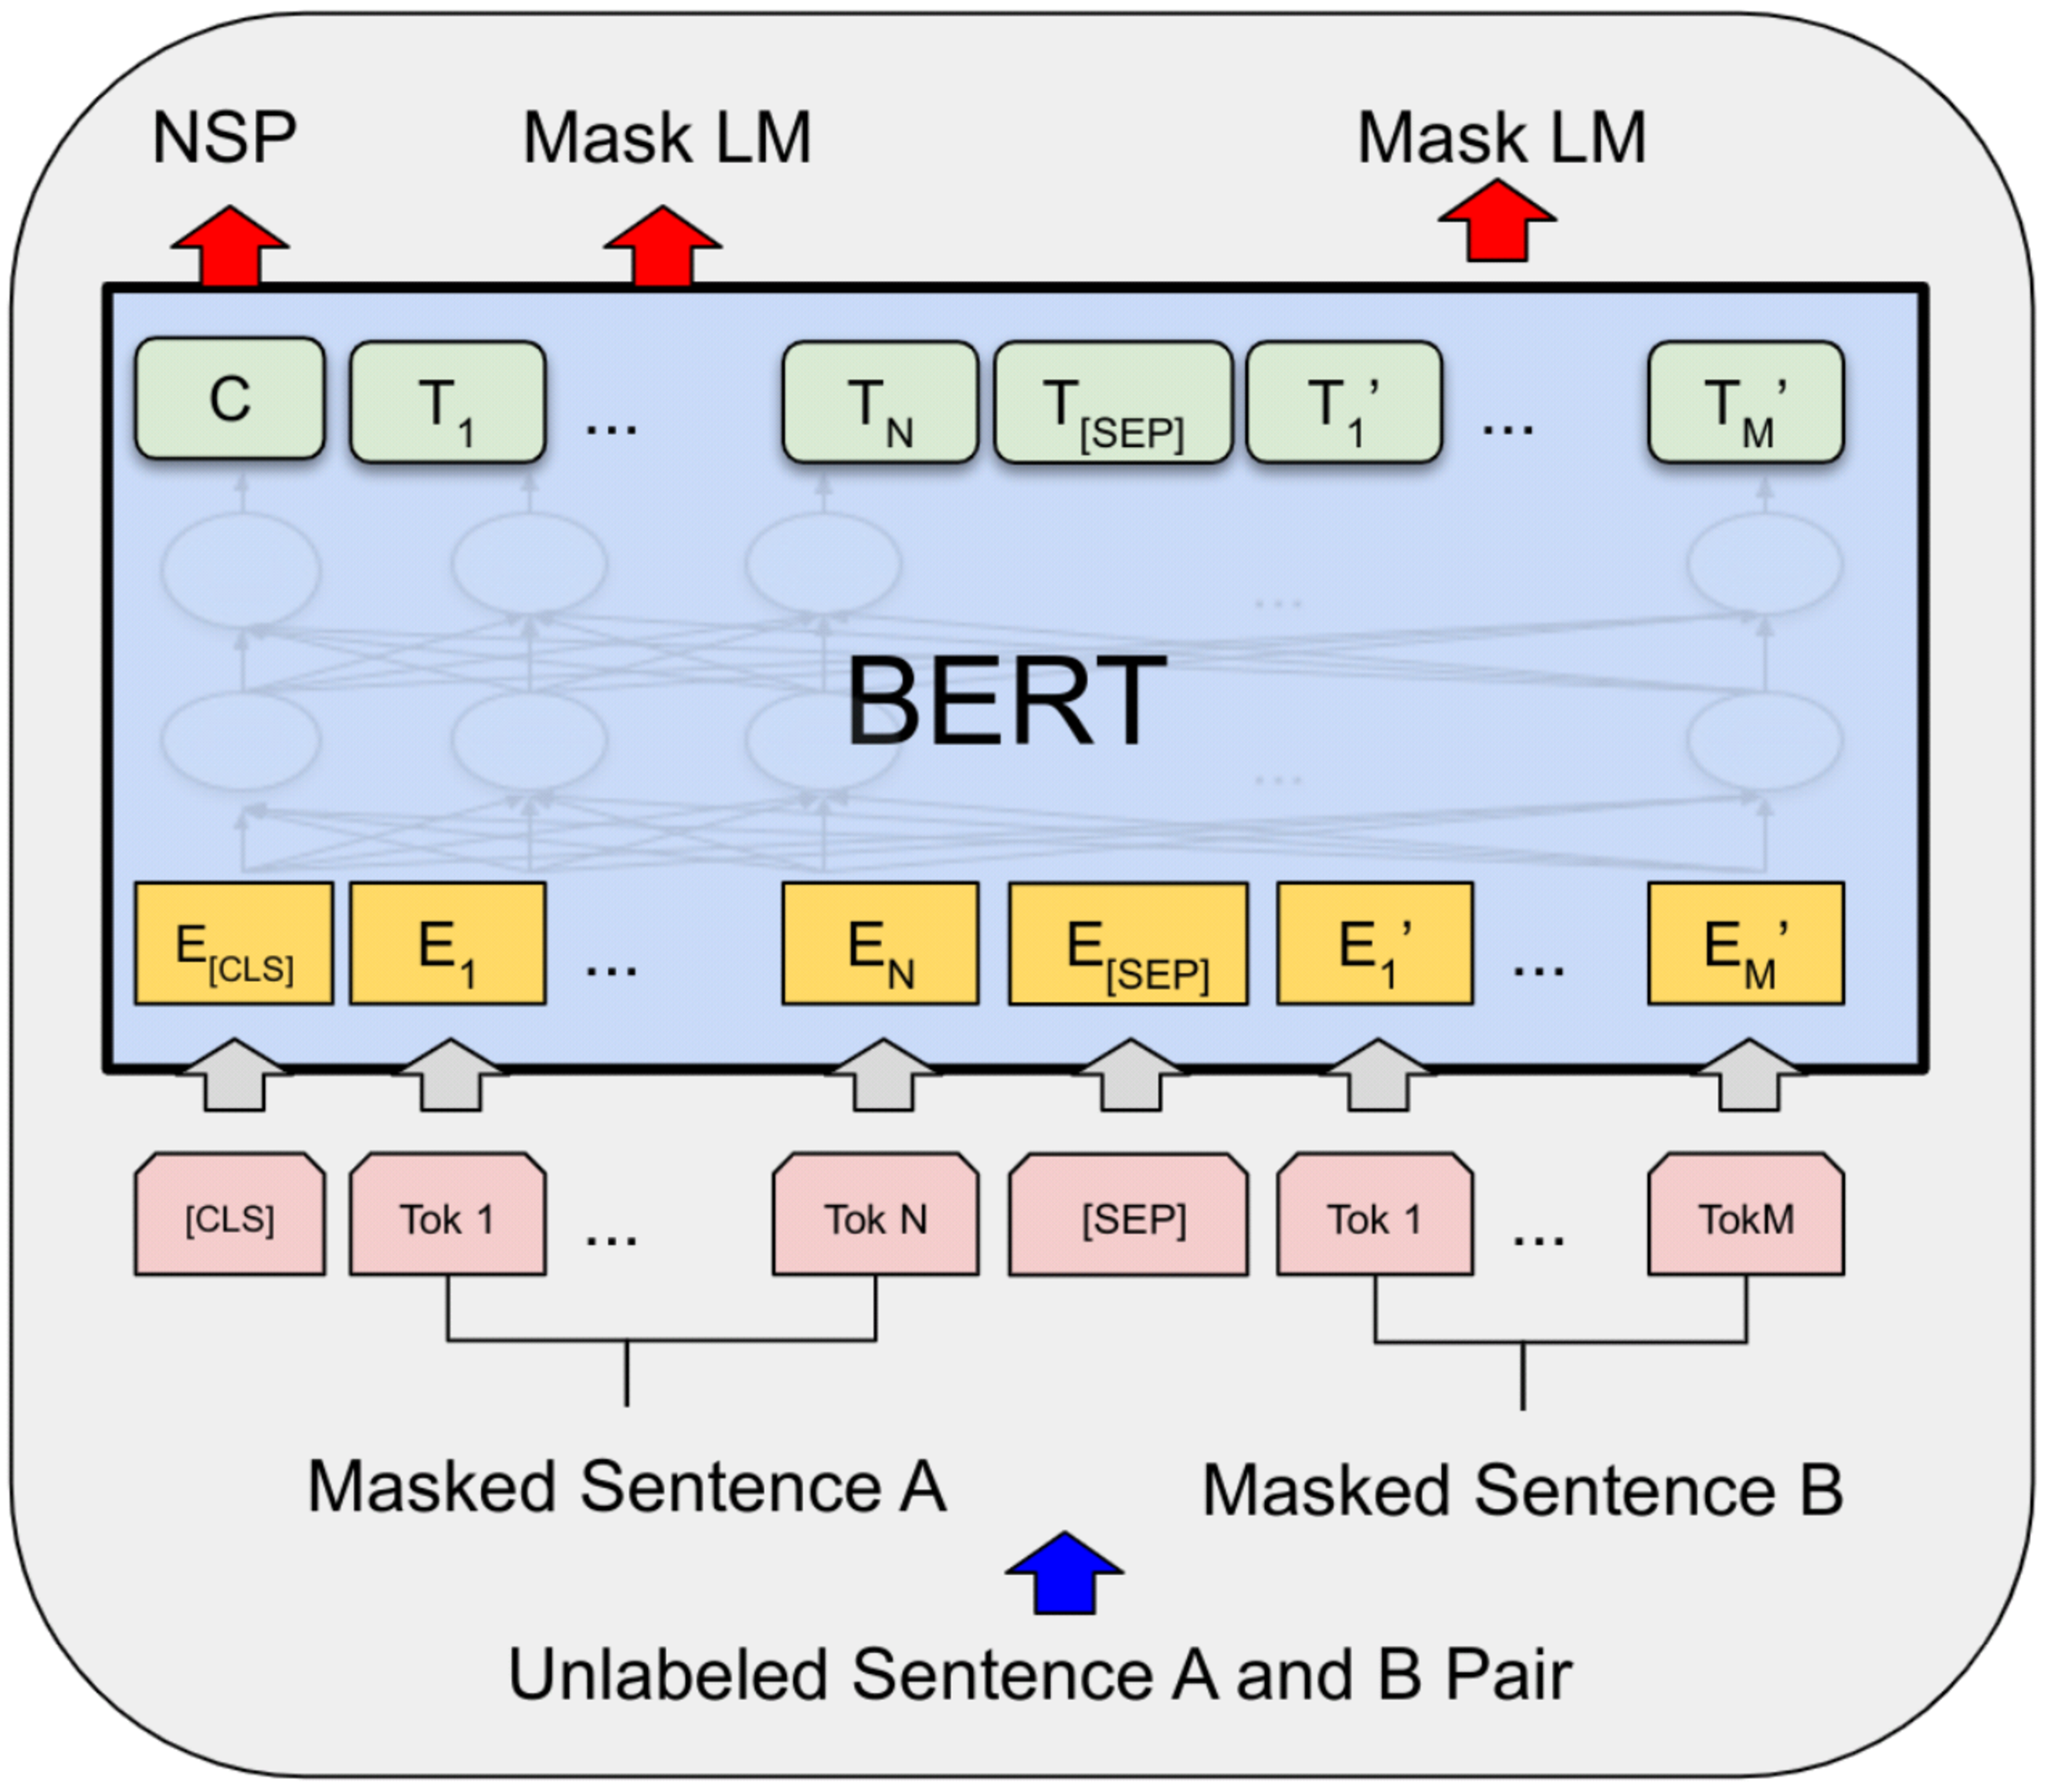
\includegraphics[width=0.6\textwidth]{img/embedders/bert/pre-training}
  \caption{Pre-Training With BERT.}
  \source{\textsc{Devlin} et al. -- BERT}
  \label{fig:pre-training}
\end{figure}

In Figure \ref{fig:pre-training}, BERT produces the hidden states of each input
token where each hidden state consists of a vector of the same size (e.g., 768
for BERT-Base) as the others, containing float numbers.  Among these hidden
states, the first position is related to the hidden state of the token
\texttt{[CLS]}. This hidden state is interesting as it determines the continuity
of two sentences, which can later be used for fine-tuning tasks.

Furthermore, the hidden states pass through a last FFN containing as many
neurons as tokens in the vocabulary used. The pre-training phase ends by
obtaining probability distribution on the hidden states using a softmax
activation function at the output of this FFN. Finally, BERT compares the
distribution of the current one-hot encoded vector token with the predicted word
and train the network using cross-entropy. It is important to note that the loss
only considers the prediction of masked tokens produced by the network to raise
awareness of the context during the network's training.

\subsection{Fine-Tuning}
\label{subsec:bert:fine-tuning}

The fine-tuning consists of training the BERT model on a specific NLP
task. Depending on the use case, either the final hidden state of the
\texttt{[CLS]} token or the hidden of the other tokens will be taken. The former
is use for classification-related tasks and the latter for more complex tasks
such as the Stanford Question Answering Dataset (SQuAD), Named Entity
Recognition (NER), and Multi-Genre Natural Language Inference (MNLI).
\begin{figure}[!ht]
  \centering
  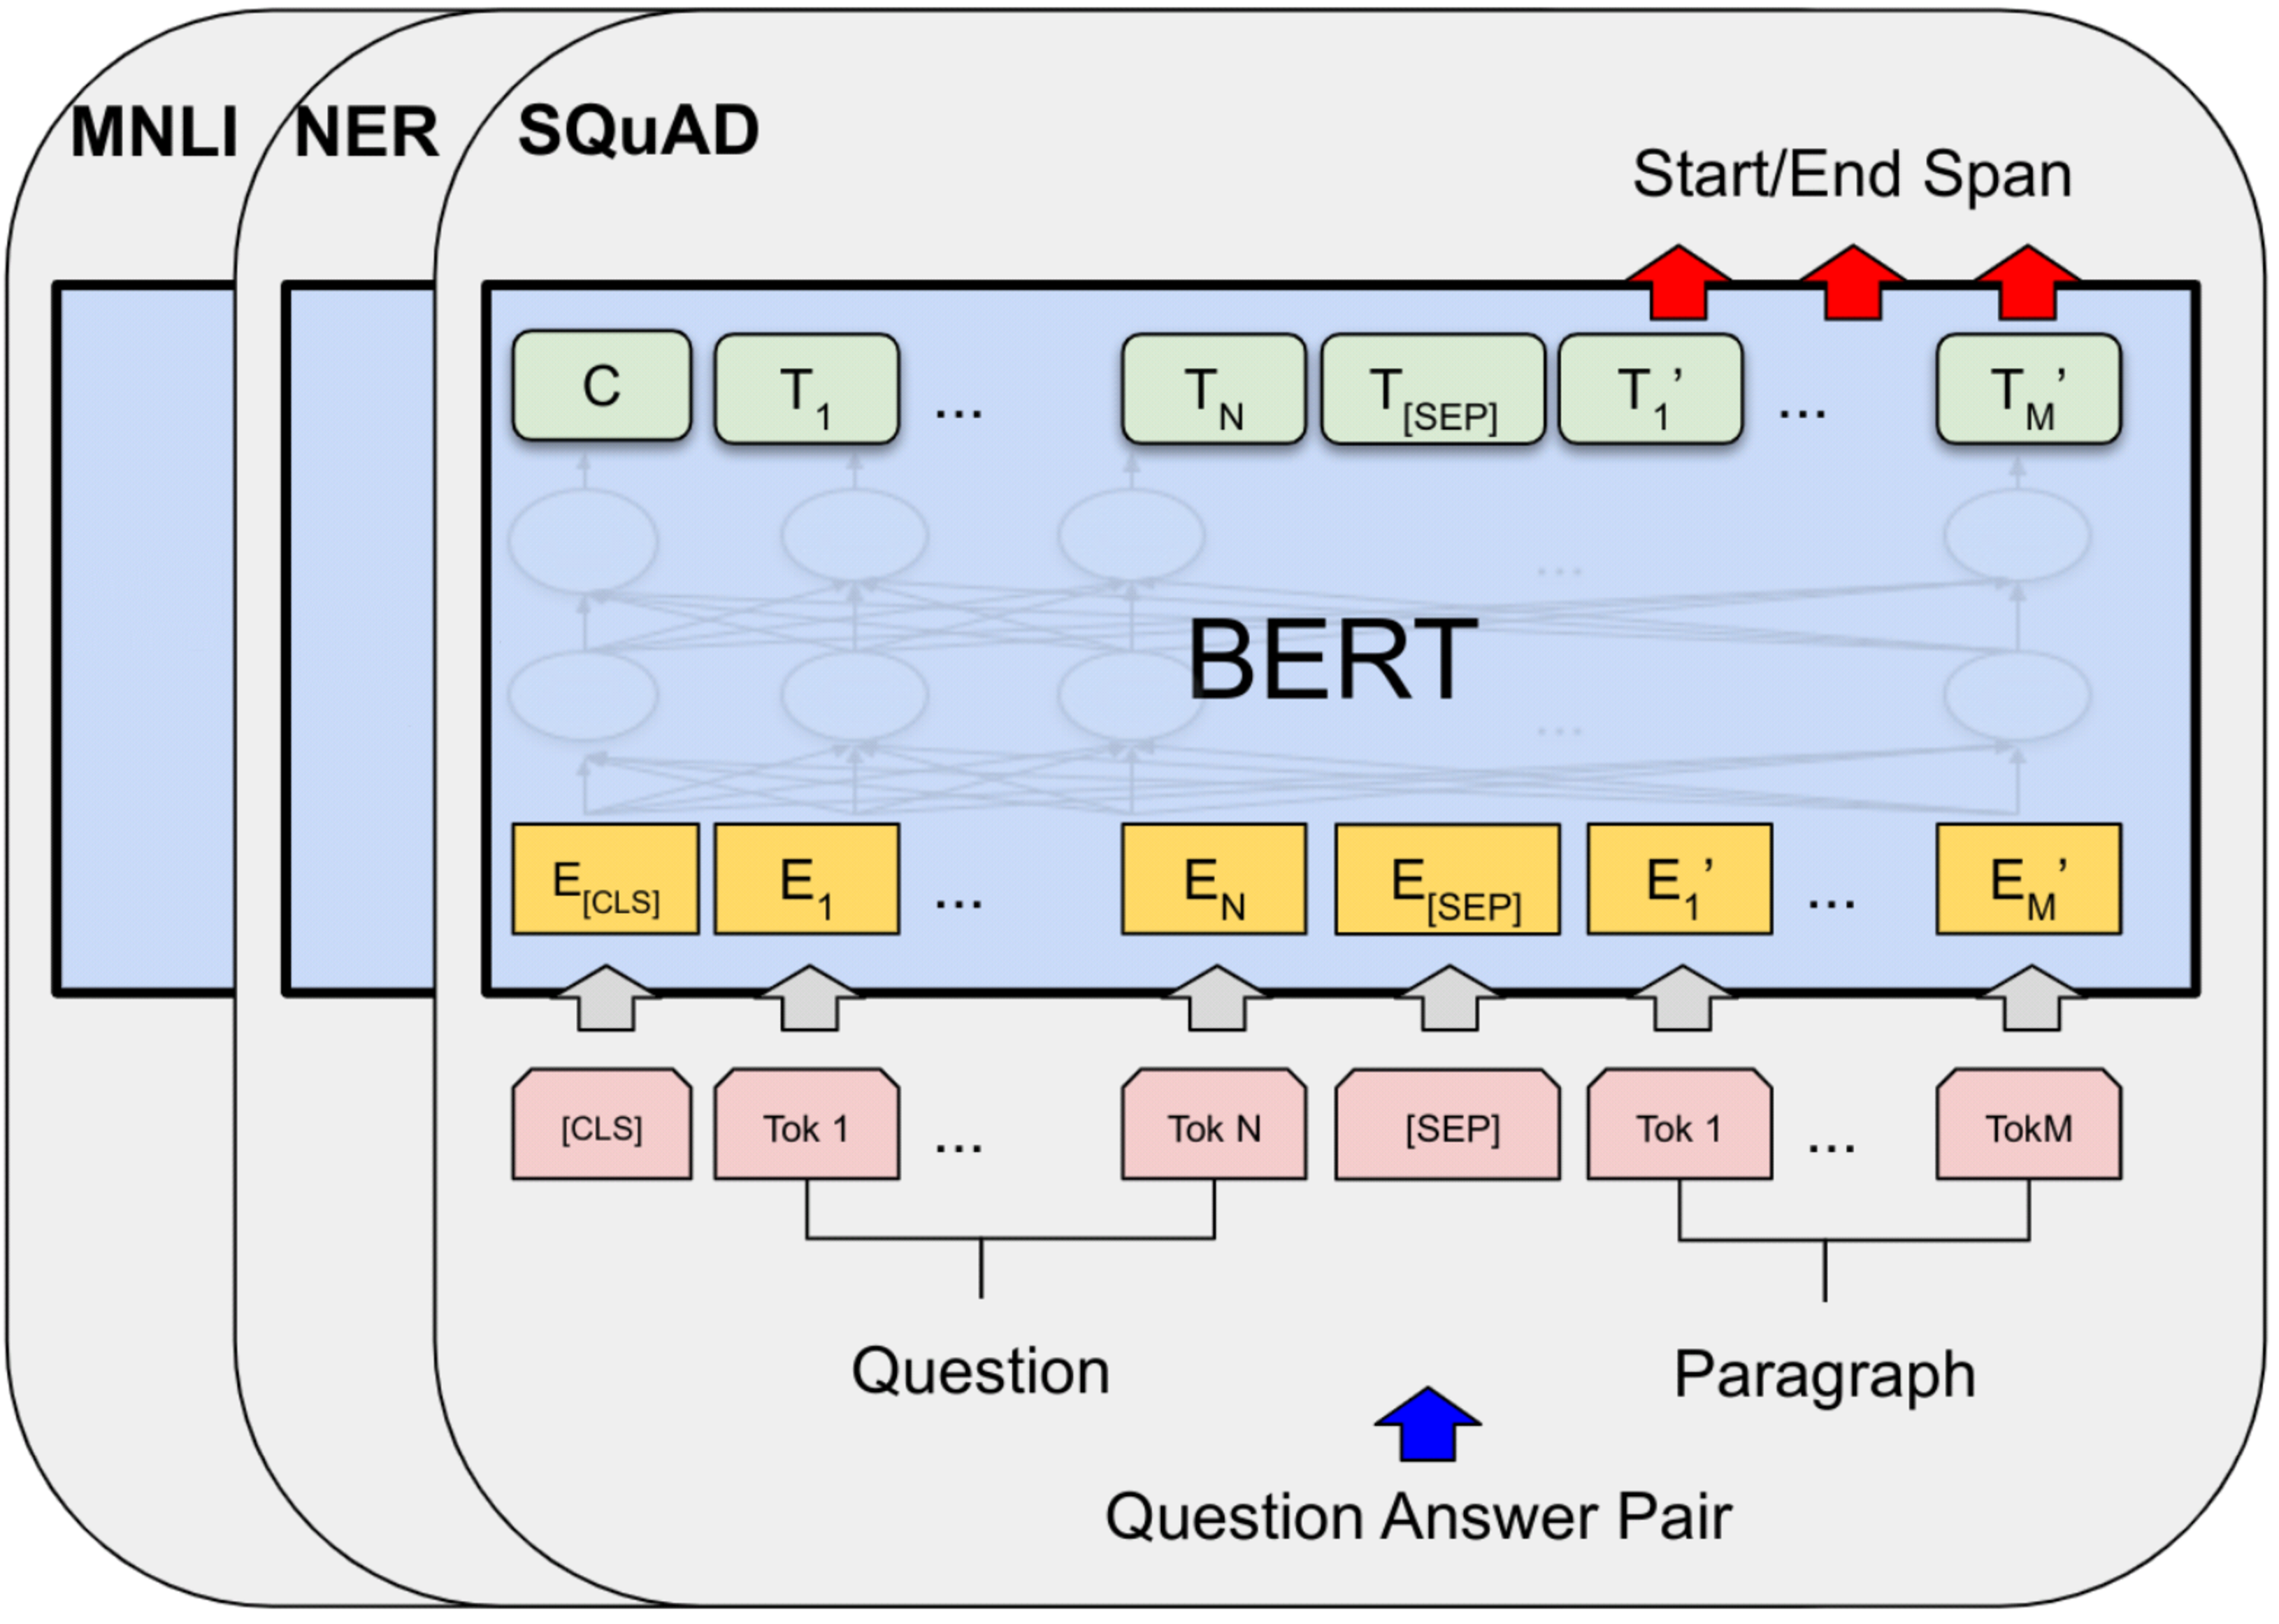
\includegraphics[width=0.7\textwidth]{img/embedders/bert/fine-tuning}
  \caption{Fine-Tuning for SQuAD.}
  \source{\textsc{Devlin} et al. -- BERT}
  \label{fig:bert:fine-tuning}
\end{figure}

In Figure \ref{fig:bert:fine-tuning}, the fine-tuning of the model for SQuAD
takes as input sequence a question and a paragraph containing the answer to this
question. Regarding the model's output for this NLP task, BERT returns the
answer to a submitted question. For this purpose, BERT highlights the starting
and ending word of a given paragraph that includes the answer to that question
only if that answer is in the paragraph. Therefore, it is interesting to look at
the probability that a word is the start/end of the answer span.

\begin{definition}[Word Probability -- Start/End of the Answer Span]
  Let $S \in \mathbb{R}^H$ be the start vector, $E \in \mathbb{R}^H$ be the end
  vector, $T_i \in \mathbb{R}^H$ be the final hidden vector for the
  i\textsuperscript{th} input token, and $j$ be the position of the ending
  word. Mathematically, the following two equations represent the probability that
  the word $i$ is the start/end of the answer span.
  \begin{equation}
    \mathrm{PS_i} = \frac{e^{ST_i}}{\sum_je^{ST_j}} \qquad \mathrm{PE_i} = \frac{e^{ET_i}}{\sum_je^{ET_j}}
    \label{eq:def:bert:word:probabilities}
  \end{equation}

  where the sum of $ST_i$ and $ET_j$ defines the score of a candidate span from
  position $i$ to position $j$. Afterward, the maximum scoring span where $j \geq
  i$ is used as a prediction.
  \label{def:squad:word:probability}
\end{definition}

The starting and ending tokens containing the answer are determined using the
softmax activation function on the dot product between the output embeddings and
the set of weights. From then on, the word with the highest probability is
assigned as the start word, and the process continues to iterate to determine
the end word. As most hyperparameters are similar to those of the pre-training,
the only new hyperparameters added during the fine-tuning concern a
classification layer. From then on, an exhaustive search of values can be done
to choose the best model according to these hyperparameters.

%%% Local Variables:
%%% mode: latex
%%% TeX-master: "../../report"
%%% End:


%%% Local Variables:
%%% mode: latex
%%% TeX-master: "../report"
%%% End:


\chapter{RDF2Vec}
\label{chap:rdf2vec}

Resource Description Framework To Vector (RDF2Vec) is an unsupervised and
task-agnostic algorithm to numerically represent nodes of a KG in an embedding
matrix that downstream ML tasks can use. RDF2Vec is unsupervised as it only
relies on the neighborhood of an entity to create embeddings and therefore does
not require any information about the node labels. Precisely, the dimensions
(e.g., $K \times 500$) of this embedding matrix result from the walk extraction
(e.g., $K$) and vector size (e.g., 500).

\section{Walk Extraction}
\label{sec:rdf2vec:walk:extraction}

This algorithm starts using a \emph{walking strategy} on a provided KG to
extract these walks, collecting an $n$-tuple of nodes starting with a root node
following a sequence of predicates and objects. Using the similarities shared by
natural language and graphs, these walks then serve as sentences for existing
NLP techniques, such as Word2Vec, to learn the embeddings of the root nodes of
this KG provided by a user.

\begin{figure}[!ht]
  \centering
  \subfloat[Step I]{
    \begin{tikzpicture}[minimum size=2cm,node distance=1cm]
      \node[entity,fill=myblue,font=\large,scale=0.6] (john) {\textsc{John}};
      \node[entity,font=\large,left=of john,scale=0.6] (friendOf){friendOf};
      \node[entity,font=\large,left=of friendOf,scale=0.6] (smith) {\textsc{Smith}};
      \node[entity,font=\large,right=of john,scale=0.6] (hasCat) {hasCat};
      \node[entity,font=\large,right=of hasCat,scale=0.6] (felix) {\textsc{Felix}};

      \draw[arrow] (john) -- node[midway,yshift=0.4cm] {\small{2}} (hasCat);
      \draw[arrow] (hasCat) -- node[midway,yshift=0.4cm] {\small{1}} (felix);
      \draw[arrow] (john) -- node[midway,yshift=0.4cm] {\small{1}} (friendOf);
      \draw[arrow] (friendOf) -- node[midway,yshift=0.4cm] {\small{1}} (smith);
    \end{tikzpicture}
  }
  \vfill
    \subfloat[Step II]{
    \begin{tikzpicture}[minimum size=2cm,node distance=1cm]
      \node[entity,font=\large,scale=0.6] (john) {\textsc{John}};
      \node[entity,font=\large,left=of john,scale=0.6] (friendOf){friendOf};
      \node[entity,font=\large,left=of friendOf,scale=0.6] (smith) {\textsc{Smith}};
      \node[entity,fill=myblue,font=\large,right=of john,scale=0.6] (hasCat) {hasCat};
      \node[entity,font=\large,right=of hasCat,scale=0.6] (felix) {\textsc{Felix}};

      \draw[arrow] (john) -- node[midway,yshift=0.4cm] {\small{2}} (hasCat);
      \draw[arrow] (hasCat) -- node[midway,yshift=0.4cm] {\small{1}} (felix);
      \draw[arrow] (john) -- node[midway,yshift=0.4cm] {\small{1}} (friendOf);
      \draw[arrow] (friendOf) -- node[midway,yshift=0.4cm] {\small{1}} (smith);
    \end{tikzpicture}
  }
  \vfill
  \subfloat[Step III]{
    \begin{tikzpicture}[minimum size=2cm,node distance=1cm]
      \node[entity,font=\large,scale=0.6] (john) {\textsc{John}};
      \node[entity,font=\large,left=of john,scale=0.6] (friendOf){friendOf};
      \node[entity,font=\large,left=of friendOf,scale=0.6] (smith) {\textsc{Smith}};
      \node[entity,font=\large,right=of john,scale=0.6] (hasCat) {hasCat};
      \node[entity,fill=myblue,font=\large,right=of hasCat,scale=0.6] (felix) {\textsc{Felix}};

      \draw[arrow] (john) -- node[midway,yshift=0.4cm] {\small{2}} (hasCat);
      \draw[arrow] (hasCat) -- node[midway,yshift=0.4cm] {\small{1}} (felix);
      \draw[arrow] (john) -- node[midway,yshift=0.4cm] {\small{1}} (friendOf);
      \draw[arrow] (friendOf) -- node[midway,yshift=0.4cm] {\small{1}} (smith);
    \end{tikzpicture}
  }
  \caption{Walk Extraction for an Oriented Graph.}
  \label{fig:rdf2vec:walk:extraction}
\end{figure}

In Figure \ref{fig:rdf2vec:walk:extraction}, a KG is composed of five nodes and
four edges. Each edge is related to a weight determined by a \emph{sampling
strategy} that can assign these weights either randomly or guided by a
particular metric, called \emph{biased walks}. These edge weights are helpful to
the walking strategy to identify the following neighboring entity to extract
in a walk. The walk extraction starts with \texttt{John} as the root node,
including \texttt{friendOf} and \texttt{hasCat} as possible candidates for the
next hop. However, as the \texttt{hasCat} edge has a higher weight than the
\texttt{friendOf} edge, the hop to \texttt{hasCat} is preferred. After this hop,
the walking strategy updates its list of candidates with the neighbors of the
current node. Finally, the process continues to iterates until this walking
strategy returns an exhaustive list of walks or reaches a specified predefined
depth covering the number of successive tuples within a walk. From then on,
there is the extraction of the 3-tuple (\texttt{John}, \texttt{hasCat},
\texttt{Felix}) walk.

The original RDF2Vec implementation uses a random walking strategy to extract a
limited number. The particularity of this walking strategy implies the
extraction of a random hop\footnote{Originally RDF2Vec preferred a random walk.}
when neighboring hops have the same weight. The random walking strategy applies
two algorithms to extract walks: the Depth-first search (DFS) and Breadth-first
search (BFS). The former traverses a graph as deep as possible before retracing
its steps. In contrast, the latter crosses every neighboring node of the same
depth before crossing those of a different depth. Therefore, if there is a
necessity to extract a specific number of walks, DFS is used by this
strategy. Otherwise, the random walker strategy picks BFS to extract every walks
of a KG.

\subsection{Walking Strategies}
\label{subsec:rdf2vec::walking:strategies}

After the publication of RDF2Vec, several walking strategies became
available~\citep{inproceedings:cochez}, where every walking strategy can be an
extraction (\texttt{type 1}) or transformation (\texttt{type 2}) technique
~\citep{article:vandewiele}. Each of these strategies brings its particularity,
making it preferable to choose them in at least one use case.

As the name implies, extraction techniques focus on extracting walks, usually so
that these walks provide richer information to produce a model resulting in the
highest possible accuracy. This category includes random walking strategy and
\emph{Community Hops}. Based on relationships not explicitly modeled in a KG,
the latter groups' nodes with similar properties through community detection. However,
both walking strategies rely on the BFS and DFS algorithms, including or not
some variations.

The transformation techniques categorize the walking strategies that transform
the extracted walks provided by a \texttt{type 1} walking strategy. As they are
easier to implement, this type includes more walking strategies than
\texttt{type 1}. This technique's primary purpose is to define
\emph{one-to-many} or \emph{many-to-one} cardinality between the old node's
labels and the new ones. If there is a \texttt{one-to-one} cardinality, no
additional information is gained and the original walking strategy could be
used.

In a non-exhaustive way, the following walking strategies of \texttt{type 2}
rely on the transformation of randomly extracted walks:
\begin{itemize}
\item \textbf{Anonymous Walk}: transforms each vertex name other than the root
node into positional information to anonymize the randomly extracted walks.

\item \textbf{Hierarchical Random Walks} (\textbf{HALK}): removes rare hops from randomly
extracted walks, increasing the quality of the generated embeddings while
reducing memory usage.

With this strategy, the suppression of a walk occurs when this walk only
contains the root node following one or more infrequent hop(s), as it will not
provide additional information.

\item \textbf{N-Gram}: transforms the $n$-grams in random walks to define a
mapping from \emph{one-to-many}. The intuition behind this strategy is that the
predecessors of a node that two different walks have in common can be different.

\item \textbf{Walklets}: transforms randomly extracted walks into walklets which
are walks of size one or two, including the root node and potentially another
node that can be a predicate or an object.

\item \textbf{Weisfeiler-Lehman}: transforms the nodes of the extracted random
walks, providing additional information about the entity representations only
when a maximum number of walks is not specified.
\end{itemize}

However, the implementations of these sampling strategies in \texttt{pyRDF2Vec}
relied on extracting child nodes, not parent nodes, which lost context for a
root node.

\subsection{Sampling Strategies}
\label{subsec:rdf2vec:sampling:strategies}

The sampling strategies essentially allow to better deal with larger KGs. A
naive implementation randomly samples a fixed number of walks for each entity to
keep the total number of walks limited. Since then, the
community~\citep{inproceedings:cochez,article:mukherjee,article:taweel} has
suggested several metrics to compute the sampling weights while walking.

Although sampling strategies allow the extraction of large KGs, most of these
strategies require working on the entire KG to assign weights to edges. However,
some KGs are so large that they need to be stored in a
\emph{triplestore}\footnote{Database designed for the storage and retrieval of
RDF.} and made available through a SPARQL endpoint. Therefore, one way to use
these sampling strategies is to load parts of large KGs, assign weights, and
start the walk extraction. Finally, the different walks extracted for these
parts of KGs would be concatenated and returned.

\section{Shortcomings}
\label{sec:rdf2vec:shortcomings}

The node representation made by RDF2Vec has already achieved great predictive
performances on several data sets in various fields. However, RDF2Vec still has
a few shortcomings. In a non-exhaustive way:
\begin{itemize}
\item \textbf{RDF2Vec does not scale to large KGs}: the walk extraction grows
exponentially with the predefined depth. This behavior is unacceptable with KGs
containing many nodes, mainly when these KGs contain many highly connected
nodes.

\item \textbf{RDF2Vec cannot deal with literals in the KG}: this algorithm
extracts node as \emph{non-ordinal categorical} data, which discard a
considerable amount of rich information that \emph{literals} can provide. In
other words, nodes can be from different types, but RDF2Vec extracts these nodes
as a name without any classification instead of conserving their types.

\item \textbf{RDF2Vec cannot deal with dynamic graphs}: adding a new entity in a
KG implies re-training the model generated by the embedding technique. This
re-training is undesirable, especially when the training time of a model is
substantial.

\item \textbf{RDF2Vec uses a simple data structure for storing walks}:
Extracting more complex data structures, such as trees, or modifying the walking
algorithm to introduce different inductive \emph{biases} could result in higher
quality embeddings. Consequently, these quality embeddings would improve the
model's accuracy.

\item \textbf{RDF2Vec uses an embedding technique that is no longer state of the
art in NLP}: currently, RDF2Vec uses Word2Vec as an embedding
technique. However, more recent NLP techniques such as BERT could be a better
alternative to Word2Vec and improve the model's accuracy.
\end{itemize}

The community has proposed solutions to address the shortcomings mentioned above
to improve this representation of nodes. Among these, optimization mechanisms
(e.g., caching and multiprocessing) to better handle large KGs and an
\emph{online learning} implementation to update the vocabulary of nodes learned
by RDF2Vec. In addition, a user could extract interesting literals by specifying
a sequence of predicates followed by a walking strategy. Finally, other
embedding techniques than Word2Vec were also proposed, such as
\emph{KGloVe}\footnote{\url{https://datalab.rwth-aachen.de/embedding/KGloVe/}},
which uses the Global Vectors for Word Representation (GloVe) embedding
technique.

%%% Local Variables:
%%% mode: latex
%%% TeX-master: "latex"
%%% End:


\chapter{Work Performed}
\label{chap:work:performed}

This chapter is dedicated to the solutions provided by this Master's
thesis. These solutions include:
\begin{itemize}
\item \textbf{Improving the accuracy of the Word2Vec model}: using a user-defined
depth to extract the child and parent nodes of a current node for each walk. In
addition, the centralization of the root node in the extracted walks
maximizes the number of training samples containing this root node and therefore
generates better quality embeddings.
\item \textbf{A BERT implementation}: builds its vocabulary only based on
special tokens and single extracted nodes, not allowing WordPiece splitting in
the tokenization of nodes. Finally, this version of BERT only considers
the MLM as a pre-training step, with training that tends to find a trade-off
between its time and the accuracy that this model will generate.
\item \textbf{A FastText implementation}: unlike its original version, its
implementation does not allow splitting $n$-grams on a defined minimum and maximum
length, but only according to a splitting function provided by a user. In
addition, the reimplementation of the Cython $n$-grams computation function in
Python to facilitate the use of \texttt{pyRDF2Vec} on Google
Colaboratory\footnote{Website that allows to run code on Google's cloud
servers.}.
\item \textbf{WideSampler}: sampling strategy that maximizes the extraction of
  shared features between entities.
\item \textbf{SplitWalker}: walking strategy that extracts walks according to a
  splitting function.
\item \textbf{A better architecture}: the \texttt{pyRDF2Vec} library now allows
to easily add walking strategies, sampling strategies, and embedding techniques
by reimplementing only a few functions.
\end{itemize}

Finally, this Master's thesis implicitly proposes some research for future work
related to BERT. Among these, the injection of \texttt{(subject, object)}
2-tuples in BERT instead of two walks. Such an injection would allow BERT to
focus to predict predicates instead of seeing correlations between two different
walks.

\section{Improving the Accuracy of the Word2Vec Model}
\label{sec:work:performed:word2vec}

To better understand how it is possible to improve the model's accuracy
generated by Word2Vec, it is helpful to consider the initial problem with the
walk extraction. With RDF2Vec, the transformation for a $n$-tuple without any walks
limitation and concerning {\footnotesize\texttt{"URL\#Alice"}} as the root node
can be achieved with each walking strategy as follows:
\begin{table}[!ht]
  \centering
  \begin{threeparttable}[t]
    \centering
    \resizebox{\textwidth}{!}{%
      \begin{tabular}{cll}
        \toprule
        \textbf{Walking Strategy} & \textbf{Initial/Transformed $\mathbf{n}$-tuple} \\
        \midrule
        \multirow{2}{*}{Anonymous Walk} & {\footnotesize\texttt{("URL\#Alice", "URL\#knows","URL\#Bob")}} \\
        & {\footnotesize\texttt{("URL\#Alice", "1", "2")}} \\
        \midrule
        \multirow{2}{*}{HALK} & {\footnotesize\texttt{("URL\#Alice", "URL\#knows", "URL\#Bob")}, \texttt{("URL\#Alice", "URL\#loves", "URL\#Bob")},} $\dotsc$ \\
        & {\footnotesize\texttt{("URL\#Alice", "URL\#knows","URL\#Bob")}}\tnote{\textcolor{blueLink}{1}} \\
        \midrule
        \multirow{2}{*}{N-Gram} & {\footnotesize\texttt{("URL\#Alice", "URL\#knows", "URL\#Bob")}, \texttt{("URL\#Alice", "URL\#loves", "URL\#Dean")}} \\
        & {\footnotesize\texttt{("URL\#Alice", "URL\#knows", "0")}, \texttt{("URL\#Alice", "URL\#loves", "1")}}\tnote{\textcolor{blueLink}{2}} \\
        \midrule
        \multirow{2}{*}{Walklets} & {\footnotesize\texttt{("URL\#Alice", "URL\#knows","URL\#Bob")}} \\
        & {\footnotesize\texttt{("URL\#Alice", "URL\#knows")}, \texttt{("URL\#Alice", "URL\#Bob")}} \\
        \midrule
        \multirow{2}{*}{Weisfeiler-Lehman} & {\footnotesize\texttt{("URL\#Alice", "URL\#knows","URL\#Bob")}} \\
        & {\footnotesize\texttt{("URL\#Alice", "URL\#knows", "URL\#Bob")}, \texttt{("URL\#Alice", "URL\#knows", "URL\#Bob-URL\#knows")}}\tnote{\textcolor{blueLink}{3}} \\
        \bottomrule
      \end{tabular}
    }%
    \begin{tablenotes}
    \item[1]
      Assuming a minor threshold frequency and an infrequent
      {\footnotesize\texttt{"URL\#loves"}} hop compared to \\ other hops.
    \item[2] Assuming at least one gram to relabel. If grams $> 2$, every object
      names will remain \\ identical for this example.
    \item[3] Assuming a Weisfeiler Lehman iteration of 1.
    \end{tablenotes}
  \end{threeparttable}%
  \caption{Example of $n$-tuple Transformation for Type 2 Walking Strategies.}
  \label{tab:walking:strategies}
\end{table}

The walking strategies in Table \ref{tab:walking:strategies} already give good
results. However, the {\footnotesize\texttt{"URL\#Alice"}} root node is always
positioned at the beginning of each walk, reducing the richness of these walks
for embedding techniques like Word2Vec, which works with window size. As the
solicitation of nodes placed in the middle of a walk is higher due to selecting
context words, including the root node as close as possible to the middle for
each walk could generate better quality embeddings. Indeed, much more training
sampling would contain this root node.

In addition to this positioning issue of the root node, \texttt{type 1} walking
strategies have the main disadvantage of continuously extracting child nodes of
a root node. In other words, the embedding techniques never know the root node's
parents. An alternative would be to extract the whole child and parent nodes of
a root node. Such extraction maximizes the extracted walk information and,
therefore, improves a model's accuracy after being trained with an embedding
technique. However, this alternative is not suitable when extracted walks are
limited, mainly used to process large KGs. Furthermore, when it comes to
positioning, the extraction of parent nodes from a root node also implies a
wrong positioning. Specifically, this root node would be this time placing as
the last node of walks, preceded by a sequence of predicates and objects, which
is not desirable.

Based on these constraints, this Master's thesis proposes to apply a
user-defined depth to extract the child and parent nodes of a current node for
each walk. Assuming that the root node has parent nodes, each extracted walk
will have a better position for this root node. Indeed, each root node will be
preceded by a part of its parent nodes and succeeded by a part of its child
nodes.

In Table \ref{tab:window:size}, assuming the sentence ``I will always remember
her'' and considering the word ``I'' as the root node of a walk, the latter is
only included twice in the context words. However, suppose now this word is
positioned in the center instead of the word "always". In that case, its
frequency of occurrence can be doubled, i.e., from two to four times for this
example. As a result, the embeddings generated for the different root nodes are
of better quality by the number of occurrence of root nodes and by the context
provided.

\section{BERT Implementation}
\label{sec:bert:implementation}

The recommended library to implement BERT is
\texttt{huggingface/transformers}\footnote{\url{https://huggingface.co/transformers/}}
which provides many pre-trained
models\footnote{\url{https://huggingface.co/models}} and essential functions to
create a model. As no pre-training model exists for BERT with KGs, it is
necessary to create this model from scratch, which requires three main steps:
\begin{enumerate}
\item \textbf{Build the vocabulary}: based on the nodes, including one line per
  special token and one line per unique node, as part of a KG.
\item \textbf{Fits the BERT model}: based on the corpus of walks provided, including three main goals:
  \begin{multicols}{2}
    \begin{enumerate}
    \item \textbf{Node tokenization}: in such a way that special tokens are
      inserted on both sides of the nodes, taking care not to split them. Which unlike
      words, splitting a URI is not desired.
    \item \textbf{Pre-training}: only done with MLM, as the NSP pre-training
      task is not helpful since the walks do not share any continuity.
    \item \textbf{Training}: is done by providing a training set of formatted
      walks, a data collator (e.g., \texttt{DataCollatorForLanguageModeling}), and the
      training parameters. The walk formatting is necessary to ensure added
      padding, truncating walks that are too long ($\geq$ 512 characters).
    \end{enumerate}
  \end{multicols}
\item \textbf{Transforms the provided entities into embeddings}: returns entity embeddings.
\end{enumerate}

\begin{lstlisting}[caption=Creation of the Walk Data Set.,label=bert:walk:dataset]
class WalkDataset(Dataset):
  def __init__(self, corpus, tokenizer):
    self.walks = [
      tokenizer(
        " ".join(walk), padding=True, truncation=True, max_length=512
      )
      for walk in corpus
    ]

  def __len__(self):
    return len(self.walks)

  def __getitem__(self, i):
    return self.walks[i]
\end{lstlisting}

In Algorithm \ref{bert:walk:dataset}, creating the walks data set for BERT
is done by creating a dedicated class. Within this class, tokenization is necessary.
Each walk is truncated to 512 characters, followed by padding to handle
walks of the same size. Finally, it is also useful to implement the
Dunder\footnote{Also called \emph{magic} methods.}  \texttt{\_\_len\_\_} and
\texttt{\_\_getitem\_\_} methods to define the size of a sample of training data
and for the fetching of this sample.

\begin{lstlisting}[caption=Creation of Node Vocabulary.,label=bert:node:vocabulary]
def _build_vocabulary(self, nodes, is_update = False):
  with open(self.vocab_filename, "w") as f:
    if not is_update:
      for token in ["[PAD]", "[UNK]", "[CLS]", "[SEP]", "[MASK]"]:
        f.write(f"{token}\n")
        self._vocabulary_size += 1
    for node in nodes:
      f.write(f"{node}\n")
      self._vocabulary_size += 1
\end{lstlisting}

In Algorithm \ref{bert:node:vocabulary}, each walk node is stored in a file with
special tokens at the beginning of the file, namely: \texttt{[PAD]},
\texttt{[UNK]}, \texttt{[CLS]}, \texttt{[SEP]}, and \texttt{[MASK]}. Finally, a
boolean is also sent to update or not an already existing vocabulary and avoid
the complete re-training of the model.

\begin{lstlisting}[caption=Fitting the BERT Model According to the Provided Walks.,label=bert:fit]
def fit(self, walks, is_update = False):
  walks = [walk for entity_walks in walks for walk in entity_walks]
  nodes = list({node for walk in walks for node in walk})
  self._build_vocabulary(nodes, is_update)
  self.tokenizer = BertTokenizer(
    vocab_file=self.vocab_filename,
    do_lower_case=False,
    never_split=nodes,
  )
  self.model_ = BertForMaskedLM(
    BertConfig(
      vocab_size=self._vocabulary_size,
      max_position_embeddings=512,
      type_vocab_size=1,
      )
   )
   Trainer(
     model=self.model_,
     args=self.training_args,
     data_collator=DataCollatorForLanguageModeling(
       tokenizer=self.tokenizer
     ),
     train_dataset=WalkDataset(walks, self.tokenizer),
   ).train()
 \end{lstlisting}

In Algorithm \ref{bert:fit}, the training of the BERT model consists of
retrieving each unique node from the provided walks, tokenizing these walks,
choosing a suitable hyperparameter config, and running the training based on a
set of walks data.

BERT needs to be trained on a large enough corpus of walks to provide good
results. Having such a corpus is not always possible, depending on the size of
some KGs. In addition, hyperparameters for training BERT impact the model's
accuracy and training time. This training time can take hours, days, weeks, if
not more. Therefore it is necessary to improve as much as possible the quantity
and quality of the walks corpus with RDF2Vec to reduce this training time.

\begin{lstlisting}[caption=Getting the Entities' Embeddings with BERT.,label=bert:embeddings]
def transform(self, entities):
  check_is_fitted(self, ["model_"])
  return [
    self.model_.bert.embeddings.word_embeddings.weight[
      self.tokenizer(entity)["input_ids"][1]
    ]
    .cpu()
    .detach()
    .numpy()
    for entity in entities
  ]
\end{lstlisting}

In Algorithm \ref{bert:embeddings}, the retrieving of embeddings for the
requested entities, i.e., the root notes, consists of recovering the generated
embeddings and ensuring their good formatting.

These methods are sufficient for a classical implementation of BERT. All the
subtlety of generating a correct model is characterized by the extraction and
injection of walks and the values of chosen hyperparameters.

\section{FastText Implementation}
\label{sec:fasttext:implementation}

To implement FastText, the
\texttt{gensim}\footnote{\url{https://github.com/RaRe-Technologies/gensim}}
library is recommended to be used. However, \texttt{pyRDF2Vec} had to
reimplement much of the code in order:
\begin{itemize}
\item \textbf{To remove the \texttt{min\_n} and \texttt{max\_n} parameters for $n$-grams
    splitting}: the \texttt{object} nodes in \texttt{pyRDF2Vec} are encoded in MD5
  to reduce their storage in RAM. Therefore, splitting them into $n$-grams is pointless.
\item \textbf{To allow a user to compute $n$-grams for walks only by separating} (default
  split by their symbols) \textbf{the URIs of subjects and predicates}: a user
  will likely want to provide an alternative splitting strategy for computing entity
  $n$-grams on the KG. If this is the case, \texttt{pyRDF2Vec} allows a user
  to implement this function that FastText will use.
\item \textbf{To avoid dependency on Cython}: Cython is a programming language between
Python and C. Its main interest is to obtain performances of calculation time
similar to C for specific functions in Python by reimplementing them in
Cython. The gensim library uses Cython for the calculation of n-grams
hashes. However, \texttt{pyRDF2Vec} has chosen to reimplement this function in
Python to facilitate its use on Google Colaboratory.
\end{itemize}

\begin{lstlisting}[caption=Reimplementation of the Hash Calculation Functions in
  \texttt{gensim}.,label=fasttext:hash]
  def compute_ngrams_bytes(entity):
    if "http" in entity:
      ngrams = " ".join(re.split("[#]", entity)).split()
      return [str.encode(ngram) for ngram in ngrams]
    return [str.encode(entity)]

    def ft_hash_bytes(self, bytez: bytes) -> int:
      h = 2166136261
      for b in bytez:
        h = h ^ b
        h = h * 16777619
      return h

    def ft_ngram_hashes(entity, num_buckets = 2000000):
      encoded_ngrams = func_computing_ngrams(entity)
      hashes = [ft_hash_bytes(n) % num_buckets for n in encoded_ngrams]
      return hashes

    def recalc_char_ngram_buckets(bucket, buckets_word, index_to_key) -> None:
      if bucket == 0:
        buckets_word = [np.array([], dtype=np.uint32)] * len(index_to_key)
        return
      self.buckets_word = [None] * len(index_to_key)
      for i, word in enumerate(index_to_key):
        buckets_word[i] = np.array(ft_ngram_hashes(word, 0, 0, self.bucket), dtype=np.uint32)
\end{lstlisting}

In Algorithm \ref{fasttext:hash}, the functions present in \texttt{gensim} are
reimplemented in such a way to include the splitting function of
\texttt{pyRDF2Vec}. Added to that this reimplementation does not consider the
use of Cython anymore.

\begin{lstlisting}[caption=Fitting the FastText Model According to the Provided Walks.,label=fasttext:fit]
def fit(self, walks, is_update = False):
  corpus = [walk for entity_walks in walks for walk in entity_walks]
  self._model.build_vocab(corpus, update=is_update)
  self._model.train(
    corpus,
    total_examples=self._model.corpus_count,
    epochs=self._model.epochs,
  )
  return self
\end{lstlisting}

In Algorithm \ref{fasttext:fit}, training with FastText consists of extracting
each node from each walk, building the vocabulary, and training the model based
on the corpus of walks.

\begin{lstlisting}[caption=Getting the Entity Embeddings with FastText.,label=fasttext:transform]
def transform(self, entities):
  if not all([entity in self._model.wv for entity in entities]):
    raise ValueError(
      "The entities must have been provided to fit() first "
      "before they can be transformed into a numerical vector."
    )
  return [self._model.wv.get_vector(entity) for entity in entities]
\end{lstlisting}

In Algorithm \ref{fasttext:transform}, even though FastText can generate entity
embeddings that it has not learned, \texttt{pyRDF2Vec} throws an exception
instead of avoiding any unpleasant surprises from the model’s accuracy.

\section{SplitWalker}
\label{sec:split:walker}

Based on the idea of FastText, but directly applied to the extraction of walks,
this Master's thesis proposes \texttt{SplitWalker} as a new \texttt{type
2}. Specifically, this strategy splits the vertices of the random walks for a
based entity. To achieve this, each vertex, except the root node, is split
according to symbols, capitalization, and numbers by removing any duplication.

\begin{table}[!ht]
  \centering
  \resizebox{\textwidth}{!}{%
    \begin{tabular}{cll}
      \toprule
      & \textbf{Initial Node} & \textbf{Node After Splitting} \\
      \midrule
      \multirow{4}{*}{\footnotesize Walk 1} & \footnotesize\texttt{http://dl-learner.org/carcinogenesis\#d19} & \footnotesize\texttt{http://dl-learner.org/carcinogenesis\#d19} \\
      & \multirow{2}{*}{\footnotesize\texttt{http://dl-learner.org/carcinogenesis\#hasBond}} & \footnotesize\texttt{has} \\
      & & \footnotesize\texttt{bond} \\
      & \footnotesize\texttt{http://dl-learner.org/carcinogenesis\#bond3209} &\footnotesize\texttt{3209} \\
      \midrule
      \multirow{3}{*}{\footnotesize Walk 2} & \footnotesize\texttt{http://dl-learner.org/carcinogenesis\#d19} & \footnotesize\texttt{http://dl-learner.org/carcinogenesis\#d19} \\
      & \footnotesize\texttt{http://www.w3.org/1999/02/22-rdf-syntax-ns\#type} & \footnotesize\texttt{type} \\
      & \footnotesize\texttt{http://dl-learner.org/carcinogenesis\#Compound} & \footnotesize\texttt{compound} \\
      \bottomrule
    \end{tabular}
  }%
  \caption{Example of Use of \texttt{SplitWalker}.}
  \label{work:performed:splitwalker}
\end{table}

In Table \ref{work:performed:splitwalker}, two walks are transformed by
\texttt{SplitWalker}. Both keep their root node intact. However, the first walk
has the \texttt{.../hasBond} split by the letter \texttt{B} into two nodes:
\texttt{has} and \texttt{bond}. In addition, its third node
\texttt{.../bond3209} is also split into two nodes: \texttt{bond} and
\texttt{3209}, but since \texttt{bond} is an existing node in the walk, it is
removed from it. Finally, the second walk has the particularity to have a node
with a capital letter. In this case, this node is rewritten in lowercase.

\begin{lstlisting}[caption=Splits Nodes of Random Walks with \texttt{SplitWalker}.,label=splitwalker:split]
def basic_split(self, walks):
  canonical_walks = set()
  for walk in walks:
    canonical_walk = [walk[0].name]
    for i, _ in enumerate(walk[1::], 1):
      vertices = []
      if "http" in walk[i].name:
        vertices = " ".join(re.split("[\#]", walk[i].name)).split()
      if i % 2 == 1:
        name = vertices[1] if vertices else walk[i].name
        preds = [
          sub_name
          for sub_name in re.split(r"([A-Z][a-z]*)", name)
          if sub_name
        ]
        for pred in preds:
          canonical_walk += [pred.lower()]
      else:
        name = vertices[-1] if vertices else walk[i].name
        objs = []
        try:
          objs = [str(float(name))]
        except ValueError:
          objs = re.sub("[^A-Za-z0-9]+", " ", name).split()
          if len(objs) == 1:
            match = re.match(
              r"([a-z]+)([0-9]+)", objs[0], re.I
            )
            if match:
              objs = list(match.groups())
        for obj in objs:
          canonical_walk += [obj.lower()]
    canonical_walk = list(dict(zip(canonical_walk, canonical_walk)))
    canonical_walks.add(tuple(canonical_walk))
  return canonical_walks
\end{lstlisting}

Algorithm \ref{splitwalker:split} starts by traversing each provided
walk, making sure to save the root node characterized by the first vertex of the
walk. Then, this function looks to see if that node has the prefix ``http'' for
each node. If it does, then that node is split by the \texttt{\#}
symbol. Otherwise, if the current node is a predicate, this function does an
uppercase split to create other nodes. Finally, this process is also done in the
case where the node contains numbers. In the end, this function deletes all the
duplicated nodes and returns the walks.

\section{WideSampler}
\label{sec:wide:sampler}

Based on the principle that humans tend to classify objects according to common
features (e.g., color and shape), this Master's thesis proposes a new sampling
strategy called \texttt{WideSampler}. This strategy addresses the assumption
that single entity-specific features would have a negligible impact on the
quality of the generated embeddings. \texttt{WideSampler} assigns higher weights
to edges that lead to the most significant number of predicates and objects in
the neighborhood and terms of occurrence in a graph to extract a maximum of
shared features between entities.

After training the model, this walking strategy can retrieve the weight of a
neighboring hop as shown below.
\begin{algorithm}
  \caption{\texttt{get\_weight(h, d, c)}}
  \label{alg:wide:sampler:get:weight}
  \begin{algorithmic}[1]
    \REQUIRE a $\mathcal{H}$ 2-tuple that contains a predicate and an object.
    \REQUIRE a $\mathcal{D}$ array of $n \geq 1$ degree indexed from $0$ to $n - 1$
    \REQUIRE a $\mathcal{C}$ array of $n \geq 1$ counter of neighbors indexed from $0$ to $n - 1$
    \ENSURE The weight of the hop for this predicate
    \IF{$\mathcal{D}_{preds}$ and $\mathcal{D}_{objs}$ and $\mathcal{C}$}
    \RETURN $\left(\mathcal{C}[\mathcal{H}[0]_{name}]\ +\ \mathcal{C}[\mathcal{H}[1]_{name}]\right)$ $\left(\dfrac{\mathcal{D}_{preds}[\mathcal{H}[0]_{name}] + \mathcal{D}_{objs}[\mathcal{H}[1]_{name}]}{2}\right)$
    \ENDIF
  \end{algorithmic}
\end{algorithm}

Algorithm \ref{alg:wide:sampler:get:weight} assigns a weight to a
\texttt{(predicate, object)} hop according to the multiplication of two
sums. The first one considers the child nodes of a predicate and the parent
nodes of an object node. The second one considers the number of occurrences of
this predicate and this node in the whole KG. Finally, the second sum is divided
by half to provide a slight preference to a hop that reaches multiples nodes.

\newpage

\begin{algorithm}
  \caption{\texttt{fit(v)}}
  \label{alg:wide:sampler:fit}
  \begin{algorithmic}[1]
    \REQUIRE an $\mathcal{V}$ array of $n \geq 1$ edges indexed from $0$ to $n - 1$
    \ENSURE Fits the WideSampler sampling strategy
    \STATE $\mathcal{C}_{objs}$ $\leftarrow$ new array of $n$ objects.
    \STATE $\mathcal{C}_{preds}$ $\leftarrow$ new array of $n$ predicates.
    \FORALL{$vertex \in \mathcal{V}$}
    \IF{$vertex$ is predicate}
    \STATE $\mathcal{C}_{neighbors}[vertex_{name}] = |\texttt{get\_children(vertex)}|$
    \STATE $\mathcal{C}_{tmp} \leftarrow \mathcal{C}_{preds}$
    \ELSE
    \STATE $\mathcal{C}_{neighbors}[vertex_{name}] = |\texttt{get\_parents(vertex)}|$
    \STATE $\mathcal{C}_{tmp} \leftarrow \mathcal{C}_{objs}$
    \ENDIF

    \IF{$vertex_{name}$ in $\mathcal{C}_{tmp}$}
    \STATE $\mathcal{C}_{tmp}[vertex_{name}] \leftarrow \mathcal{C}[vertex_{name}] + 1$
    \ELSE
    \STATE $\mathcal{C}_{tmp}[vertex_{name}] \leftarrow 1$
    \ENDIF
    \ENDFOR
  \end{algorithmic}
\end{algorithm}

Algorithm \ref{alg:wide:sampler:fit} trains the \texttt{WideSampler} strategy by
iterating through a set of vertices. Depending on the vertex, the algorithm
considers the number of children or parents of this vertex. If it is a
predicate, then the number of its child nodes is stored in a counter. Otherwise,
the algorithm stores the number of parent nodes in another counter. Finally, the
number of occurrences of each identical vertex in the whole KG is also
collected.

\section{Library Architecture}
\label{sec:pyRDF2Vec}

\texttt{pyRDF2Vec}\footnote{\url{https://github.com/IBCNServices/pyRDF2Vec}} is
the Python library created by IDLab that allows to use RDF2Vec. Through the
internship and this Master's thesis, this library has undergone many changes in
its architecture to improve its use.
\begin{figure}[!ht]
  \centering
  \resizebox{\linewidth}{!} {
    \begin{tikzpicture}[>=stealth',
      extract_walks/.style={draw,minimum width=.8cm,minimum height=.8cm,fill=mygreen!40},
      process/.style={draw,minimum width=1cm,minimum height=1cm,node distance=0.35cm,fill=mybrown!20}
      ]
    \node[draw,minimum width=2.5cm,minimum height=3cm,loosely dashed,color=darkBlue] at (0,0) (graph_entities) {};
    \node[draw,minimum width=2cm,minimum height=1cm,yshift=-65pt,above=of graph_entities,fill=myblue] (graph) {Graph};
    \node[draw,minimum width=2cm,minimum height=1cm,yshift=15pt,below=of graph,fill=myblue] (entities) {Entities};
    \node[draw,minimum width=2cm,minimum height=1cm,yshift=2pt,above=of graph,fill=myblue!50] (connector) {Connector};

    \node[inner sep=0pt,xshift=-20pt,above=of connector] (rdf) {
\includegraphics[width=0.074\textwidth]{img/rdf}};
    \node[inner sep=0pt,xshift=20pt,above=of connector] (sparql) {
\includegraphics[width=0.08\textwidth]{img/sparql}};

    \node[label,below of=graph_entities,yshift=-1.1cm,color=darkBlue] {\textbf{Inputs}};

    \node[draw,minimum width=3cm,minimum height=1cm,right=of graph_entities,fill=myyellow] (transformer) {Transformer};
    \node[draw,minimum width=2.5cm,minimum height=3cm,loosely dashed,color=darkRed,right=of transformer] (walker_sampler) {};
    \node[draw,minimum width=2cm,minimum height=1cm,yshift=-65pt,above=of walker_sampler,fill=myred] (walker) {Walker};
    \node[draw,minimum width=2cm,minimum height=1cm,yshift=15pt,below=of walker,fill=myred] (sampler) {Sampler};
    \node[draw,minimum width=3cm,minimum height=1cm,above=of transformer,fill=mypurple!50] (embedder) {Embedder};
    \node[draw,ellipse,minimum width=3cm,minimum height=1cm,above=of embedder,fill=mypurple] (embeddings) {Embeddings};
    \node[draw,ellipse,minimum width=3cm,minimum height=1cm,node distance=0.5cm,right=of embeddings,fill=mypurple] (literals) {Literals};

    \node[label,above of=walker_sampler,xshift=0.3cm,yshift=20pt,color=darkRed] {\textbf{Strategy}};

    \node[inner sep=0pt,xshift=-50pt,above right=of embeddings] (sklearn) {
\includegraphics[width=0.15\textwidth]{img/scikit-learn}};

    \node[process,node distance=9cm,right=of connector] (p1) {P1/T1};

    \node[process,below=of p1] (p2) {P2/T2};
    \node[process,below=of p2] (p3) {P3/T3};
    \node[process,below=of p3] (p4) {P4/T4};

    \node[extract_walks,right=of p1] (extract_walks_1) {Extract Walks};
    \node[extract_walks,right=of p2] (extract_walks_2) {Extract Walks};
    \node[extract_walks,right=of p3] (extract_walks_3) {Extract Walks};
    \node[extract_walks,right=of p4] (extract_walks_4) {Extract Walks};

    \node[draw,minimum width=7.5cm,minimum height=1.5cm,xshift=1.8cm,yshift=-2.3cm,above=of embeddings,loosely dashed,color=darkPurple] (output) {};
    \node[label,above of=output,xshift=2.5cm,yshift=-0.1cm,color=darkPurple] {\textbf{Outputs}};

    \node[label,below of=p4,yshift=-0.10cm] {\dots};
    \node[label,below of=extract_walks_4,yshift=-0.10cm] {\dots};

    \node[draw,ellipse,minimum width=3cm,minimum height=1cm, node distance=8cm,right=of walker,fill=mygreen] (walks) {Walks};

    \draw[arrow,shorten >=0.2cm,shorten <=0.2cm] (transformer) -- (walker_sampler) node[midway,above] {(2)};

    \draw[arrow,shorten >=0.2cm,shorten <=0.2cm] (rdf.south) -- ([xshift=-20pt]connector.north);
    \draw[arrow,shorten >=0.2cm,shorten <=0.2cm] (sparql.south) -- ([xshift=20pt]connector.north);
    \draw[arrow,shorten >=0.05cm,shorten <=0.2cm] (connector) -- (graph);

    \draw[arrow,shorten >=0.2cm,shorten <=0.2cm] (p1) -- (extract_walks_1);
    \draw[arrow,shorten >=0.2cm,shorten <=0.2cm] (p2) -- (extract_walks_2);
    \draw[arrow,shorten >=0.2cm,shorten <=0.2cm] (p3) -- (extract_walks_3);
    \draw[arrow,shorten >=0.2cm,shorten <=0.2cm] (p4) -- (extract_walks_4);

    \draw[arrow,shorten >=0.2cm,shorten <=0.2cm] (literals) -- (sklearn);

    \draw[shorten <=0.1cm] ([yshift=12pt]walker.east) -| ([xshift=-20pt]p1.west);
    \draw[arrow,shorten >=0.1cm] ([xshift=-20pt]p1.west) -- (p1.west);

    \draw[shorten <=0.1cm] ([yshift=4pt]walker.east) -| ([xshift=-15pt]p2.west);
    \draw[arrow,shorten >=0.1cm] ([xshift=-15pt]p2.west) -- (p2.west);

    \draw[shorten <=0.1cm] ([yshift=-4pt]walker.east) -| ([xshift=-15pt]p3.west);
    \draw[arrow,shorten >=0.1cm] ([xshift=-15pt]p3.west) -- (p3.west);

    \draw[shorten <=0.1cm] ([yshift=-12pt]walker.east) -| ([xshift=-20pt]p4.west);
    \draw[arrow,shorten >=0.1cm] ([xshift=-20pt]p4.west) -- (p4.west);

    \draw[shorten <=0.1cm] (extract_walks_1.east) -| ([xshift=-15pt,yshift=12pt]walks.west);
    \draw[arrow,shorten >=0.1cm] ([xshift=-15pt,yshift=12pt]walks.west) -- ([yshift=12pt]walks.west);

    \draw[shorten <=0.1cm] (extract_walks_2.east) -| ([xshift=-20pt,yshift=4pt]walks.west);
    \draw[arrow,shorten >=0.1cm] ([xshift=-20pt,yshift=4pt]walks.west) -- ([yshift=4pt]walks.west);

    \draw[shorten <=0.1cm] (extract_walks_3.east) -| ([xshift=-20pt,yshift=-4pt]walks.west);
    \draw[arrow,shorten >=0.1cm] ([xshift=-20pt,yshift=-4pt]walks.west) -- ([yshift=-4pt]walks.west);

    \draw[shorten <=0.1cm] (extract_walks_4.east) -| ([xshift=-15pt,yshift=-12pt]walks.west);
    \draw[arrow,shorten >=0.1cm] ([xshift=-15pt,yshift=-12pt]walks.west) -- ([yshift=-12pt]walks.west);

    \draw[arrow,shorten >=0.1cm,shorten <=0.1cm] (sampler) -- (walker);
    \draw[arrow,shorten >=0.2cm,shorten <=0.2cm] (transformer) -- (embedder) node[midway,right] {(3)};
    \draw[arrow,shorten >=0.05cm,shorten <=0.2cm] (embedder) -- (embeddings);
    \draw[arrow,shorten >=0.2cm,shorten <=0.2cm] (embeddings) -- (sklearn);

    \draw[arrow,shorten >=0.2cm,shorten <=0.2cm] (graph_entities) -- (transformer.west) node[midway,above] {(1)};

    \draw[shorten <=0.2cm] ([xshift=0.2cm]transformer) -- ([yshift=1.3cm]walker_sampler.north);
    \draw[arrow,shorten >=0.05cm] ([yshift=1.3cm]walker_sampler.north) -- (literals);

    \draw ([xshift=10pt]walks.east) |- ([yshift=-20pt]extract_walks_4.south);
    \draw[shorten <=0.1cm] (walks) -- ([xshift=10pt]walks.east);
    \draw[arrow,shorten >=0.2cm] ([yshift=-20pt]extract_walks_4.south) -| (transformer.south);
  \end{tikzpicture}
  }
  \caption{Workflow of \texttt{pyRDF2Vec}.}
  \label{tikz:workflow}
\end{figure}

In Figure \ref{tikz:workflow}, the workflow of \texttt{pyRDF2Vec} includes three
primary operations and is divided into seven main consecutive significant
blocks:
\begin{multicols}{2}
\begin{enumerate}
\item \textbf{Connector}: in charge of interaction with a local or remote graph.
\item \textbf{Graph}: in charge of providing a graph encoding the knowledge-based.
\item \textbf{Entities}: in charge of provides the entities in a
\texttt{rdflib.URI.term} or \texttt{str} type to generate the embeddings.
\item \textbf{Transformer}: in charge of converting graphs into embeddings for
downstream ML tasks, using a walking strategy and sampling strategy and an
embedder.
\item \textbf{Sampler}: in charge of prioritizing the use of some paths over
others using a weight allocation strategy.
\item \textbf{Walker}: in charge of extracting walks in a KG from provided
entities and optionally from a sampling strategy using multiple
processors/threads.
\item \textbf{Embedder}: in charge of training a model with an embedding
technique using extracted walks and therefore generate embeddings of entities
provided by a user.
\end{enumerate}
\end{multicols}

The design of such architecture allows having a long-term vision. Due to this
architecture, a user can contribute to \texttt{pyRDF2Vec} and easily add new
walking strategies and sampling and embedding techniques. For this Master’s
thesis, implementing this architecture was necessary to facilitate the
comparison of embedding techniques. Each new embedding technique is added in an
\texttt{Embedder} package and must reimplement the \texttt{fit} and
\texttt{get\_weight} functions of the \texttt{Embedder} class.

%%% Local Variables:
%%% mode: latex
%%% TeX-master: "latex"
%%% End:


\chapter{Benchmarks}
\label{chap:benchmarks}

For these benchmarks, only the maximum number of walks per entity and the
maximum depth per walk is varied. Furthermore, due to a time issue (cf. Section
\ref{sec:objectives:problems}) these benchmarks are performed on \texttt{MUTAG},
a graph of moderate size composed of
\SI{74567}{triples}\footnote{\textbf{SELECT} (COUNT(*) AS ?triples)
\textbf{WHERE} \{ ?s ?p ?o \}} \SI{22534}{entities }\footnote{\textbf{SELECT}
(COUNT(\textbf{DISTINCT} ?s) AS ?entities) \textbf{WHERE} \{ ?s a \}}, and
\SI{24}{relations}\footnote{\textbf{SELECT} (COUNT(\textbf{DISTINCT} ?p) AS
?relations) \textbf{WHERE} \{ ?s ?p ?o \}}. Finally, each value entered in these
benchmarks is the result of the average of five values.

\section{Setup}
\label{sec:setup}

Benchmarks related to embeddings techniques and walking strategies are directly
launched on IDLab's\footnote{Research group of imec.} servers with \SI{4}{CPUs},
\SI{64}{\giga\byte} RAM, and one GPU. Those related to sampling strategies are
launched directly on a ThinkPad machine with \SI{4}{CPUs} and
\SI{16}{\giga\byte} of RAM. This physical device change is made since, except
for \texttt{UniformSampler}, the sampling strategies only work on locally stored
KGs. As the IDLab servers interact with the KGs via SPARQL endpoints, they were
not used for these benchmarks. Finally, the benchmarks use 340 training entities
and attempt to predict 68 test entities, which is a standard for \texttt{MUTAG}.

\section{Results}
\label{sec:results}

This section contains the results of the different embedding techniques, walking
strategies, and sampling strategies for \texttt{MUTAG}.


\subsection{Embedding Techniques}
\label{subsec:embedding:techniques}

FastText, BERT and Word2Vec are trained on the basis of ten epochs. In addition,
FastText and Word2Vec use twenty negative words with a vector size of 500. For
its splitting function, FastText uses a primary splitting function where the
\texttt{\#} symbol splits each entity Finally, each embedding technique uses a
\texttt{RandomWalker} and an \texttt{UniformSampler}.

About the training of BERT, the latter is only trains on
\texttt{MUTAG}. However, in case of multiple KGs, it is important to re-train it
for each different KGs. Similarly, if BERT is trained with too few walks, it
will be necessary to retrain it with a larger number of walks. In this case,
online learning is important to avoid to retrain the whole model which can be
time-consuming. Unline BERT that can take hours, days for training the model,
Word2Vec and FastText take a few minutes to tens of minutes to train, which is
significant difference.

\begin{table}[!ht]
  \centering
  \begin{tabular}{rl}
    \toprule
    \textbf{Hyperparameter} & \textbf{Value} \\
    \midrule
    \textbf{Epochs} & 10 \\
    \textbf{Warmup Steps} & 500 \\
    \textbf{Weight Decay} & 0.01 \\
    \textbf{Learning Rate} & 2e-5 \\
    \textbf{Batch Size} & 16 \\
    \bottomrule
  \end{tabular}
  \caption{Basic Hyperparameters Used for Training the BERT Model.}
  \label{tab:bert:hyperparameters}
\end{table}

In Table \ref{tab:bert:hyperparameters}, The values of these basic
hyperparameters were chosen after several tests using a Grid Search with Cross
Validation and depending on the training time. More precisely, a training of the
BERT model with these hyperparameters with MUTAG and the same hardware
characteristics as those of the IDLab servers, is done between 25 minutes and
few hours.

\begin{table}[!ht]
  \centering
  \resizebox{\textwidth}{!}{%
    \begin{tabular}{cccS[table-format=2.2]@{${}\pm{}$}S[table-format=1.1]c}
      \toprule
      \textbf{Embedding Technique} & \textbf{Max. Depth} & \textbf{Max. Walks}
      & \multicolumn{2}{c}{\textbf{Accuracy} (\SI{}{\percent})} & \textbf{Rank} \\
      \midrule
      \texttt{FastText(negative=20,vector\_size=500)} & \multirow{3}{*}{2} & \multirow{3}{*}{250} & 79.71 & 2.35 & 1 \\
      \texttt{Word2Vec(negative=20,vector\_size=500)} & & & 76.76 & 1.71 & 2 \\
      \texttt{BERT(learning\_rate=2e-5,batch\_size=16)} & & & 70.59 & 5.88 & 3 \\
      \midrule
      \texttt{FastText(negative=20,vector\_size=500)} & \multirow{3}{*}{4} & \multirow{3}{*}{250} & 77.06 & 1.50 & 1 \\
      \texttt{Word2Vec(negative=20,vector\_size=500)} & & & 75.00 & 1.61 & 2 \\
      \texttt{BERT(learning\_rate=2e-5,batch\_size=16)} & & & 74.26 & 2.21 & 3 \\
      \midrule
      \texttt{FastText(negative=20,vector\_size=500)} & \multirow{3}{*}{6} & \multirow{3}{*}{250} & 82.35 & 1.86 & 1 \\
      \texttt{BERT(learning\_rate=2e-5,batch\_size=16)} & & & 76.32 & 3.24 & 2 \\
      \texttt{Word2Vec(negative=20,vector\_size=500)} & & & 74.71 & 2.35 & 3 \\
      \bottomrule
    \end{tabular}
  }%
  \caption{Evaluation of the Embedding Techniques for \texttt{MUTAG} According
    to the Maximum Depth per Walk.}
  \label{benchmarks:embedders:mutag:depth}
\end{table}

In Table \ref{benchmarks:embedders:mutag:depth}, regardless of the maximum depth
per walk chosen for the same number of walks per entity, FastText indicates a
model's accuracy above Word2Vec. Specifically, FastText allows an average
increase of the model's accuracy of 4.22 times the one given by Word2Vec. In
addition, FastText provides an excellent model's accuracy with \texttt{MUTAG}
for a maximum depth per walk of 6. For BERT, the latter shows better results for
larger maximum depth per walk.

\begin{figure}[!ht]
  \centering
  \resizebox{\textwidth}{!}{%
  \begin{tikzpicture}
    \begin{axis}[
      scale only axis,
      grid=major,
      grid style={dashed,gray!30},
      height=6cm,
      width=9cm,
      legend cell align={left},
      legend entries={
        \footnotesize{\texttt{BERT(learning\_rate=2e-5,batch\_size=16)}},
        \footnotesize{\texttt{Word2Vec(negative=20,vector\_size=500)}},
        \footnotesize{\texttt{FastText(negative=20,vector\_size=500)}}
      },
      legend style={
        legend pos=outer north east,
        font=\small
      },
      ylabel={Accuracy},
      xlabel={Maximum Depth per Walk},
      xtick={2,4,6},
      ytick={75,77,79.70,82.30},
      ]

      \addplot[red,mark=*,error bars/.cd, y dir=both, y explicit]
      table[x=max_depth,y=accuracy,col sep=comma] {data/embedders/max-depth/bert.csv};
      \addplot[blue,mark=*,error bars/.cd, y dir=both, y explicit]
      table[x=max_depth,y=accuracy,col sep=comma] {data/embedders/max-depth/word2vec.csv};
      \addplot[green,mark=*,error bars/.cd, y dir=both, y explicit]
      table[x=max_depth,y=accuracy,col sep=comma] {data/embedders/max-depth/fasttext.csv};
    \end{axis}
  \end{tikzpicture}
  }%
  \caption{Evaluation of the Embedding Techniques for \texttt{MUTAG} According
    to the Maximum Depth per Walk.}
  \label{fig:benchmarks:embedders:depth}
\end{figure}

In Figure \ref{fig:benchmarks:embedders:depth}, the curves of Word2Vec and
FastText have an almost identical trajectory, except for a maximum depth per
walk of 6. In this case, the accuracy model of FastText increases, while the
accuracy model of Word2Vec decreases. Finally, BERT's accuracy is proportional
to the maximum depth per walk. As well as the time needed to train the model.

\begin{table}[!ht]
  \centering
  \resizebox{\textwidth}{!}{%
    \begin{tabular}{cccS[table-format=2.2]@{${}\pm{}$}S[table-format=1.2]c}
      \toprule
      \textbf{Embedding Technique} & \textbf{Max. Depth} & \textbf{Max. Walks}
      & \multicolumn{2}{c}{\textbf{Accuracy} (\SI{}{\percent})} & \textbf{Rank} \\
      \midrule
      \texttt{FastText(negative=20,vector\_size=500)} & \multirow{3}{*}{4} & \multirow{3}{*}{100} & 77.94 & 1.61 & 1 \\
      \texttt{Word2Vec(negative=20,vector\_size=500)} & & & 71.47 & 2.20 & 2 \\
      \texttt{BERT(learning\_rate=2e-5,batch\_size=16)} & & & 69.43 & 1.73 & 3 \\
      \midrule
      \texttt{FastText(negative=20,vector\_size=500)} & \multirow{3}{*}{4} & \multirow{3}{*}{250} & 77.35 & 3.90 & 1 \\
      \texttt{Word2Vec(negative=20,vector\_size=500)} & & & 74.71 & 2.53 & 2 \\
      \texttt{BERT(learning\_rate=2e-5,batch\_size=16)} & & & 73.54 & 2.28 & 3 \\
      \midrule
      \texttt{FastText(negative=20,vector\_size=500)} & \multirow{3}{*}{4} & \multirow{3}{*}{500} & 76.18 & 1.71 & 1 \\
      \texttt{BERT(learning\_rate=2e-5,batch\_size=16)} & & & 75.24 & 2.37 & 2 \\
      \texttt{Word2Vec(negative=20,vector\_size=500)} & & & 73.53 & 1.86 & 3 \\
      \midrule
      \texttt{FastText(negative=20,vector\_size=500)} & \multirow{3}{*}{4} & \multirow{3}{*}{1000} & 77.35 & 2.73 & 1 \\
      \texttt{BERT(learning\_rate=2e-5,batch\_size=16)} & & & 76.58 & 1.17 & 2 \\
      \texttt{Word2Vec(negative=20,vector\_size=500)} & & & 74.41 & 3.03 & 3 \\
      \bottomrule
    \end{tabular}
  }%
  \caption{Evaluation of the Embedding Techniques for \texttt{MUTAG} According
    to the Maximum Number of Walks per Entity}
  \label{benchmarks:embedders:mutag:walks}

\end{table}

In Table \ref{benchmarks:embedders:mutag:walks}, regardless of the number of
walks chosen for the same maximum depth per walk, FastText indicates a model's
accuracy above Word2Vec. Specifically, FastText allows an average increase of
the model's accuracy of 3.675 times the one given by Word2Vec. For BERT, the
latter shows better results for larger maximum depth per walk, but performs less
well for smaller maximum depth per walk. For BERT, the latter indicates an
interesting model's accuracy for 500 and 1000 walks. However, the results are
not as exceptional for a lower maximum of walks per entity.

\begin{figure}[!ht]
  \centering
  \resizebox{\textwidth}{!}{%
    \begin{tikzpicture}
      \begin{axis}[
        scale only axis,
        grid=major,
        grid style={dashed,gray!30},
        height=6cm,
        width=9cm,
        legend cell align={left},
        legend entries={
          \footnotesize{\texttt{BERT(learning\_rate=2e-5,batch\_size=16)}},
          \footnotesize{\texttt{Word2Vec(negative=20,vector\_size=500)}},
          \footnotesize{\texttt{FastText(negative=20,vector\_size=500)}}
        },
        legend style={
          legend pos=outer north east,
          font=\small
        },
        ylabel={Accuracy},
        xlabel={Maximum Number of Walks per Entity},
        xtick={100,250,500,1000},
        ytick={71.50,73.50,74.50,76.20,78}
        ]

        \addplot[red,mark=*,error bars/.cd, y dir=both, y explicit]
        table[x=max_walk,y=accuracy,col sep=comma] {data/embedders/max-walks/bert.csv};
        \addplot[blue,mark=*,error bars/.cd, y dir=both, y explicit]
        table[x=max_walk,y=accuracy,col sep=comma] {data/embedders/max-walks/word2vec.csv};
        \addplot[green,mark=*,error bars/.cd, y dir=both, y explicit]
        table[x=max_walk,y=accuracy,col sep=comma] {data/embedders/max-walks/fasttext.csv};
      \end{axis}
    \end{tikzpicture}
  }%
  \caption{Evaluation of the Embedding Techniques for \texttt{MUTAG} According
    to the Maximum Number of Walks per Entity.}
  \label{fig:benchmarks:embedders:walks}
\end{figure}

In Figure \ref{fig:benchmarks:embedders:walks}, the curves of Word2Vec and
FastText still have an almost identical trajectory, except for a maximum number
of walks per entity of 250. In this case, the accuracy model of Word2Vec
increases, while the accuracy model of FastText decreases. Finally, BERT's
accuracy is also proportional to the maximum number of walks per entity. As well
as the time needed to train the model.

\newpage

\begin{table}[!ht]
  \centering
  \begin{tabular}{lc}
    \toprule
    \textbf{Embedding Technique} & \textbf{Average Rank} \\
    \midrule
    \texttt{FastText(negative=20,vector\_size=500)} & 1 \\
    \texttt{Word2Vec(negative=20,vector\_size=500)} & 2 \\
    \texttt{BERT(learning\_rate=2e-5,batch\_size=16)} & 3 \\
    \bottomrule
  \end{tabular}
  \caption{Evaluation of the Average Rank of the Embedding Techniques for \texttt{MUTAG}.}
  \label{tab:benchmark:embedders:average:rank}
\end{table}

In Figure \ref{tab:benchmark:embedders:average:rank}, Word2Vec is the winning
embedding techniques in these benchmarks for \texttt{MUTAG}, followed by
FastText, and BERT.

%%% Local Variables:
%%% mode: latex
%%% TeX-master: "../../master-thesis"
%%% End:


\subsection{Walking Strategies}
\label{subsec:walkers}

Each walking strategy is evaluated using \texttt{UniformSampler} as sampling strategy and
Word2Vec as embedding technique. For these benchmarks, Word2Vec keeps the same
hyperparameters as given in Section \ref{subsec:embedding:techniques}, namely
ten epochs, twenty negative words and a vector size of 500.

\begin{table}[!ht]
  \centering
  \resizebox{\textwidth}{!}{%
    \begin{tabular}{lccS[table-format=2.2]@{${}\pm{}$}S[table-format=1.2]c}
      \toprule
      \textbf{Walker} & \textbf{Max. Depth} & \textbf{Max. Walks}
      & \multicolumn{2}{c}{\textbf{Accuracy} (\SI{}{\percent})} & \textbf{Rank} \\
      \midrule
      \texttt{RandomWalker} & \multirow{6}{*}{2} & \multirow{6}{*}{250} & \textbf{77.94} & 2.08 & 1 \\
      \texttt{NGramWalker(grams=3)} & & & 76.47 & 1.32 & 2 \\
      \texttt{HALKWalker(freq\_threshold=0.01)} & & & 75.59 & 2.39 & 3 \\
      \texttt{SplitWalker} & & & 74.71 & 2.53 & 4 \\
      \texttt{WalkletWalker} & & & 72.06 & 1.32 & 5 \\
      \texttt{AnonymousWalker} & & & 65.29 & 1.76 & 6 \\
      \midrule
      \texttt{HALKWalker(freq\_threshold=0.01)} & \multirow{6}{*}{4} & \multirow{6}{*}{250} & \textbf{78.82} & 1.50 & 1 \\
      \texttt{SplitWalker} & & & 77.35 & 4.01 & 2 \\
      \texttt{RandomWalker} & & & 76.76 & 6.06 & 3 \\
      \texttt{NGramWalker(grams=3)} & & & 75.88 & 3.90 & 4 \\
      \texttt{WalkletWalker} & & & 73.82 & 1.95 & 5 \\
      \texttt{AnonymousWalker} & & & 66.47 & 1.44 & 6 \\
      \midrule
      \texttt{HALKWalker(freq\_threshold=0.01)} & \multirow{6}{*}{6} & \multirow{6}{*}{250} & \textbf{81.18} & 4.87 & 1 \\
      \texttt{SplitWalker} & & & 79.71 & 2.16 & 2 \\
      \texttt{NGramWalker(grams=3)} & & & 77.65 & 1.95 & 3 \\
      \texttt{RandomWalker} & & & 75.29 & 2.16 & 4 \\
      \texttt{WalkletWalker} & & & 71.76 & 1.10 & 5 \\
      \texttt{AnonymousWalker} & & & 67.65 & 1.86 & 6 \\
      \bottomrule
    \end{tabular}
    }%
  \caption{Evaluation of the Accuracy of Walking Strategies for \texttt{MUTAG} According
    to the Maximum Depth per Walk.}
  \label{benchmarks:walkers:mutag:depth}
\end{table}

In Table \ref{benchmarks:walkers:mutag:depth}, regardless of the maximum depth
per walk chosen for the same number of walks per entity, \texttt{HALKWalker}
indicates a model's accuracy above \texttt{SplitWalker}. However, these two
walking strategies provide better results for more significant maximum depths per
walk. While \texttt{RandomWalker} indicates a good model's accuracy for small maximum
depth per walk.

\newpage

\begin{figure}[!ht]
  \centering
  \resizebox{\textwidth}{!}{%
  \begin{tikzpicture}
    \begin{axis}[
      scale only axis,
      grid=major,
      grid style={dashed,gray!30},
      height=6cm,
      width=9cm,
      legend cell align={left},
      legend entries={
        \texttt{AnonymousWalker},
        \texttt{HALKWalker(freq\_threshold=0.01)},
        \texttt{NGramWalker(grams=3)},
        \texttt{RandomWalker},
        \texttt{SplitWalker},
        \texttt{WalkletWalker},
      },
      legend style={
        legend pos=outer north east,
        font=\small
      },
      ylabel={Accuracy},
      xlabel={Maximum Depth per Walk},
      xtick={2, 4, 6},
      ytick={65.30,67,71.80,73.80,76,78,79.70,81.20},
      ]

      \addplot[brown,mark=*,error bars/.cd, y dir=both, y explicit]
      table[x=max_depth,y=accuracy,col sep=comma] {data/walkers/max-depth/anonymous.csv};
      \addplot[yellow,mark=*,error bars/.cd, y dir=both, y explicit]
      table[x=max_depth,y=accuracy,col sep=comma] {data/walkers/max-depth/halk.csv};
      \addplot[blue,mark=*,error bars/.cd, y dir=both, y explicit]
      table[x=max_depth,y=accuracy,col sep=comma] {data/walkers/max-depth/ngram.csv};
      \addplot[green,mark=*,error bars/.cd, y dir=both, y explicit]
      table[x=max_depth,y=accuracy,col sep=comma] {data/walkers/max-depth/random.csv};
      \addplot[red,mark=*,error bars/.cd, y dir=both, y explicit]
      table[x=max_depth,y=accuracy,col sep=comma] {data/walkers/max-depth/split.csv};
      \addplot[darkPurple,mark=*,error bars/.cd, y dir=both, y explicit]
      table[x=max_depth,y=accuracy,col sep=comma] {data/walkers/max-depth/walklet.csv};
    \end{axis}
  \end{tikzpicture}
  }%
  \caption{Evaluation of the Accuracy of Walking Strategies for MUTAG According to the Maximum Depth per Walk.}
  \label{fig:benchmarks:walkers:depth}
\end{figure}

In Figure \ref{fig:benchmarks:walkers:depth}, the curve of \texttt{SplitWalker}
and \texttt{HALKWalker} have an identical trajectory, except that
\texttt{HALKWalker} indicates better model's accuracy than
\texttt{SplitWalker}. In addition, they return better model's accuracy than the
other walking strategies.

\begin{table}[!ht]
  \centering
  \resizebox{\textwidth}{!}{%
    \begin{tabular}{lccS[table-format=2.2]@{${}\pm{}$}S[table-format=1.2]c}
      \toprule
      \textbf{Walker} & \textbf{Max. Depth} & \textbf{Max. Walks}
      & \multicolumn{2}{c}{\textbf{Accuracy} (\SI{}{\percent})} & \textbf{Rank} \\
      \midrule
      \texttt{SplitWalker} & \multirow{6}{*}{4} & \multirow{6}{*}{100} & \textbf{79.12} & 4.20 & 1 \\
      \texttt{HALKWalker(freq\_threshold=0.01)} & & & 77.65 & 2.53 & 2 \\
      \texttt{WalkletWalker} & & & 73.82 & 1.95 & 3 \\
      \texttt{RandomWalker} & & & 72.35 & 3.77 & 4 \\
      \texttt{NGramWalker(grams=3)} & & & 68.82 & 3.99 & 5 \\
      \texttt{AnonymousWalker} & & & 65.59 & 1.18 & 6 \\
      \midrule
      \texttt{SplitWalker} & \multirow{6}{*}{4} & \multirow{6}{*}{250} & \textbf{77.35} & 2.56 & 1 \\
      \texttt{HALKWalker(freq\_threshold=0.01)} & & & 76.76 & 3.65 & 2 \\
      \texttt{RandomWalker} & & & 76.18 & 1.71 & 3 \\
      \texttt{NGramWalker(grams=3)} & & & 73.24 & 3.40 & 4 \\
      \texttt{WalkletWalker} & & & 71.76 & 1.10 & 5 \\
      \texttt{AnonymousWalker} & & & 66.76 & 1.18 & 6 \\
      \midrule
      \texttt{HALKWalker(freq\_threshold=0.01)} & \multirow{6}{*}{4} & \multirow{6}{*}{500} & \textbf{79.12} & 3.99 & 1 \\
      \texttt{SplitWalker} & & & 77.35 & 1.50 & 2 \\
      \texttt{WalkletWalker} & & & 77.06 & 3.55 & 3 \\
      \texttt{RandomWalker} & & & 72.06 & 1.32 & 4 \\
      \texttt{NGramWalker(grams=3)} & & & 71.76 & 1.10 & 5 \\
      \texttt{AnonymousWalker} & & & 65.80 & 1.44 & 6 \\
      \bottomrule
    \end{tabular}
    }%
  \caption{Evaluation of the Accuracy of Walking Strategies for \texttt{MUTAG} According
    to the Maximum Number of Walks per Entity}
  \label{tab:benchmarks:walkers:mutag:walks}
\end{table}

In Table \ref{tab:benchmarks:walkers:mutag:walks}, regardless of the number of
walks chosen for the same maximum depth per walk, \texttt{SplitWalker} indicates
a correct model's accuracy above the average of walking
strategies. Specifically, \texttt{SplitWalker} allows an average model's
accuracy of \SI{78.53}{\percent}.

\newpage

\begin{figure}[!ht]
  \centering
  \resizebox{\textwidth}{!}{%
  \begin{tikzpicture}
    \begin{axis}[
      scale only axis,
      grid=major,
      grid style={dashed,gray!30},
      height=6cm,
      width=9cm,
      legend cell align={left},
      legend entries={
        \texttt{AnonymousWalker},
        \texttt{HALKWalker(freq\_threshold=0.01)},
        \texttt{NGramWalker(grams=3)},
        \texttt{RandomWalker},
        \texttt{SplitWalker},
        \texttt{WalkletWalker},
      },
      legend style={
        legend pos=outer north east,
        font=\small
      },
      ylabel={Accuracy},
      xlabel={Maximum Number of Walks per Entity},
      xtick={100,250,500},
      ytick={65.80,68.80,72,73.20,76,77.50,79.10},
      ]

      \addplot[brown,mark=*,error bars/.cd, y dir=both, y explicit]
      table[x=max_walk,y=accuracy,col sep=comma] {data/walkers/max-walks/anonymous.csv};
      \addplot[yellow,mark=*,error bars/.cd, y dir=both, y explicit]
      table[x=max_walk,y=accuracy,col sep=comma] {data/walkers/max-walks/halk.csv};
      \addplot[blue,mark=*,error bars/.cd, y dir=both, y explicit]
      table[x=max_walk,y=accuracy,col sep=comma] {data/walkers/max-walks/ngram.csv};
      \addplot[green,mark=*,error bars/.cd, y dir=both, y explicit]
      table[x=max_walk,y=accuracy,col sep=comma] {data/walkers/max-walks/random.csv};
      \addplot[red,mark=*,error bars/.cd, y dir=both, y explicit]
      table[x=max_walk,y=accuracy,col sep=comma] {data/walkers/max-walks/split.csv};
      \addplot[darkPurple,mark=*,error bars/.cd, y dir=both, y explicit]
      table[x=max_walk,y=accuracy,col sep=comma] {data/walkers/max-walks/walklet.csv};
    \end{axis}
  \end{tikzpicture}
  }%
  \caption{Evaluation of the Walking Strategies for Different Data Sets
    According to the Maximum Number of Walks per Entity.}
  \label{fig:benchmarks:walkers:walks}
\end{figure}

In Figure \ref{fig:benchmarks:walkers:walks}, the model's accuracy with
\texttt{SplitWalker} tends to stay around \SI{77}{\percent} after a maximum
number of walks of 250. In addition, \texttt{AnonymousWalker},
\texttt{NGramWalker}, and \texttt{RandomWalker} follow the same curve
trajectory. Specifically, they have a peak of accuracy at a maximum number of
walks per entity of 250. In contrast, the other walking strategies have a
decrease of model's accuracy at this stage.

\begin{table}[!ht]
  \centering
  \begin{tabular}{lc}
    \toprule
    \textbf{Walker} & \textbf{Average Rank} \\
    \midrule
    \texttt{HALKWalker(freq\_threshold=0.01)} & 1 \\
    \texttt{SplitWalker} & 2 \\
    \texttt{RandomWalker} & 3 \\
    \texttt{NGramWalker(grams=3)} & 4 \\
    \texttt{WalkletWalker} & 5 \\
    \texttt{AnonymousWalker} & 6 \\
    \bottomrule
  \end{tabular}
  \caption{Evaluation of the Average Rank of the Walking Strategies.}
  \label{tab:benchmark:walkers:average:rank}
\end{table}

In Figure \ref{tab:benchmark:walkers:average:rank},
\texttt{HALKWalker(freq\_threshold=0.01)} is the winning walking strategy in
these benchmarks for \texttt{MUTAG}, followed by \texttt{SplitWalker}, and
\texttt{RandomWalker}.

%%% Local Variables:
%%% mode: latex
%%% TeX-master: "../../master-thesis"
%%% End:


\subsection{Sampling Strategies}
\label{subsec:samplers}

To determine the accuracy impact of \texttt{WideSampler}, the latter is compared
to other sampling strategies in a first time using \texttt{MUTAG} where only the
number of walks and depth are variable. The number of standard entities for
\texttt{MUTAG} being fixed at 340 trained entities, 68 of these serve as testing
entities. As RDF2Vec is unsupervised, including the testing entities in the
training set is not an issue.

\newpage

\begin{table}[!ht]
  \centering
  \resizebox{\textwidth}{!}{%
    \begin{tabular}{lcc S[table-format=2.2]@{${}\pm{}$}S[table-format=1.2]c}
      \toprule
      \textbf{Sampler} & \textbf{Max. Depth} & \textbf{Max. Walks}
      & \multicolumn{2}{c}{\textbf{Accuracy} (\SI{}{\percent})} & \textbf{Rank} \\
      \midrule
      \texttt{ObjPredFreqSampler} & \multirow{13}{*}{2} & \multirow{13}{*}{100} & \textbf{78.82} & 3.17 & 1 \\
      \texttt{ObjFreqSampler} & & & 77.94 & 3.35 & 2 \\
      \texttt{PredFreqSampler(inverse=True)} & & & 77.65 & 2.35 & 3 \\
      \texttt{WideSampler} & & & 76.76 & 1.95 & 4 \\
      \texttt{ObjPredFreqSampler(inverse=True)} & & & 76.76 & 2.16 & 5 \\
      \texttt{PredFreqSampler} & & & 76.76 & 4.87 & 6 \\
      \texttt{PageRankSampler(inverse=True,split=True,alpha=0.85)} & & & 76.18 & 2.16 & 7 \\
      \texttt{PageRankSampler(alpha=0.85)} & & & 76.47 & 2.08 & 8 \\
      \texttt{UniformSampler} & & & 76.18 & 4.50 & 9 \\
      \texttt{ObjFreqSampler(inverse=True,split=True)} & & & 75.88 & 4.01 & 10 \\
      \texttt{PageRankSampler(split=True,alpha=0.85)} & & & 74.71 & 1.71 & 11 \\
      \texttt{PageRankSampler(inverse=True,alpha=0.85)} & & & 74.41 & 1.50 & 12 \\
      \texttt{ObjFreqSampler(inverse=True)} & & & 73.53 & 2.79 & 13 \\
      \midrule
      \texttt{WideSampler} & \multirow{13}{*}{2} & \multirow{13}{*}{250} & \textbf{77.35} & 1.99 & 1 \\
      \texttt{PredFreqSampler} & & & 76.18 & 3.14 & 2 \\
      \texttt{PageRankSampler(split=True,alpha=0.85)} & & & 75.88 & 1.50 & 3 \\
      \texttt{ObjFreqSampler(inverse=True,split=True)} & & & 75.88 & 3.03 & 4 \\
      \texttt{PageRankSampler(inverse=True,split=True,alpha=0.85)} & & & 75.88 & 5.06 & 5 \\
      \texttt{ObjFreqSampler(inverse=true)} & & & 75.59 & 1.99 & 6 \\
      \texttt{ObjFreqSampler} & & & 75.59 & 4.71 & 7 \\
      \texttt{ObjPredFreqSampler(inverse=True)} & & & 75.29 & 1.10 & 8 \\
      \texttt{UniformSampler} & & & 75.29 & 1.44 & 9 \\
      \texttt{ObjPredFreqSampler} & & & 75.29 & 2.35 & 10 \\
      \texttt{PageRankSampler(inverse=True,alpha=0.85)} & & & 75.00 & 2.46 & 11 \\
      \texttt{PageRankSampler(alpha=0.85)} & & & 74.12 & 1.99 & 12 \\
      \texttt{PredFreqSampler(inverse=True)} & & & 73.82 & 2.53 & 13 \\
      \midrule
      \texttt{ObjFreqSampler} & \multirow{13}{*}{2} & \multirow{13}{*}{500} & \textbf{75.29} & 2.16 & 1 \\
      \texttt{PageRankSampler(alpha=0.85)} & & & 75.00 & 0.00 & 2 \\
      \texttt{WideSampler} & & & 74.71 & 1.10 & 3 \\
      \texttt{ObjFreqSampler(inverse=True,split=True)} & & & 74.71 & 3.14 & 4 \\
      \texttt{PageRankSampler(inverse=True,alpha=0.85)} & & & 74.12 & 2.56 & 5 \\
      \texttt{ObjPredFreqSampler(inverse=True)} & & & 73.82 & 2.53 & 6 \\
      \texttt{PageRankSampler(inverse=True,split=True,alpha=0.85)} & & & 73.82 & 2.16 & 7 \\
      \texttt{PageRankSampler(split=True,alpha=0.85)} & & & 73.82 & 2.53 & 8 \\
      \texttt{ObjPredFreqSampler} & & & 73.53 & 1.32 & 9 \\
      \texttt{UniformSampler} & & & 73.53 & 2.63 & 10 \\
      \texttt{PredFreqSampler} & & & 72.65 & 2.73 & 11 \\
      \texttt{ObjFreqSampler(inverse=True)} & & & 72.65 & 2.73 & 12 \\
      \texttt{PredFreqSampler(inverse=True)} & & & 72.35 & 1.95 & 13 \\
      \bottomrule
    \end{tabular}
  }%
  \caption{Accuracy of Sampling Strategies for \texttt{MUTAG} (Part I).}
  \label{tab:benchmarks:samplers:part:1}
\end{table}

In Table \ref{tab:benchmarks:samplers:part:1}, for a maximum depth of walk of 2 with
a maximum number of walks of 250, \texttt{WideSampler} indicates the best
model's accuracy. In addition, the latter gives good precision models for a
maximum number of walks of 100 and 500.

 \begin{figure}[!ht]
  \centering
  \resizebox{0.9\textwidth}{!}{%
    \begin{tikzpicture}
      \begin{axis}[
        scale only axis,
        grid=major,
        grid style={dashed,gray!30},
        height=6cm,
        width=9cm,
        legend cell align={left},
        legend entries={
          \texttt{ObjFreqSampler(inverse=True,split=True)},
          \texttt{ObjFreqSampler(inverse=True)},
          \texttt{ObjFreqSampler},
          \texttt{ObjPredFreqSampler(inverse=True)},
          \texttt{ObjPredFreqSampler},
          \texttt{PageRankSampler(inverse=True,split=True,alpha=0.85)},
          \texttt{PageRankSampler(inverse=True,alpha=0.85)},
          \texttt{PageRankSampler(split=True,alpha=0.85)},
          \texttt{PageRankSampler(alpha=0.85)},
          \texttt{PredFreqSampler(inverse=True)},
          \texttt{PredFreqSampler},
          \texttt{UniformSampler},
          \texttt{WideSampler},
        },
        legend style={
          legend pos=outer north east,
          font=\small
        },
        ylabel={Accuracy},
        xlabel={Maximum Number of Walks per Entity},
        xtick={100,250,500},
        ytick={73,74,76,78},
        ]

        \addplot[medimumBlue,mark=diamond,error bars/.cd, y dir=both, y explicit]
        table[x=max_walk,y=accuracy,col sep=comma] {data/samplers/max-depth/2/objfreq-inv-split.csv};
        \addplot[darkBlue,mark=square,error bars/.cd, y dir=both, y explicit]
        table[x=max_walk,y=accuracy,col sep=comma] {data/samplers/max-depth/2/objfreq-inv.csv};
        \addplot[blue,mark=*,error bars/.cd, y dir=both, y explicit]
        table[x=max_walk,y=accuracy,col sep=comma] {data/samplers/max-depth/2/objfreq.csv};

        \addplot[darkRed,mark=square,error bars/.cd, y dir=both, y explicit]
        table[x=max_walk,y=accuracy,col sep=comma] {data/samplers/max-depth/2/objpredfreq-inv.csv};
        \addplot[red,mark=*,error bars/.cd, y dir=both, y explicit]
        table[x=max_walk,y=accuracy,col sep=comma] {data/samplers/max-depth/2/objpredfreq.csv};

        \addplot[mediumGreen,mark=diamond,error bars/.cd, y dir=both, y explicit]
        table[x=max_walk,y=accuracy,col sep=comma] {data/samplers/max-depth/2/pagerank-inv-split.csv};
        \addplot[darkGreen,mark=square,error bars/.cd, y dir=both, y explicit]
        table[x=max_walk,y=accuracy,col sep=comma] {data/samplers/max-depth/2/pagerank-inv.csv};
        \addplot[yellow,mark=triangle,error bars/.cd, y dir=both, y explicit]
        table[x=max_walk,y=accuracy,col sep=comma]{data/samplers/max-depth/2/pagerank-split.csv};
        \addplot[green,mark=*,error bars/.cd, y dir=both, y explicit]
        table[x=max_walk,y=accuracy,col sep=comma] {data/samplers/max-depth/2/pagerank.csv};

        \addplot[darkPurple,mark=square,error bars/.cd, y dir=both, y explicit]
        table[x=max_walk,y=accuracy,col sep=comma] {data/samplers/max-depth/2/predfreq-inv.csv};
        \addplot[purple,mark=*,error bars/.cd, y dir=both, y explicit]
        table[x=max_walk,y=accuracy,col sep=comma] {data/samplers/max-depth/2/predfreq.csv};

        \addplot[brown,mark=*,error bars/.cd, y dir=both, y explicit]
        table[x=max_walk,y=accuracy,col sep=comma] {data/samplers/max-depth/2/uniform.csv};
        \addplot[black,mark=*,error bars/.cd, y dir=both, y explicit]
        table[x=max_walk,y=accuracy,col sep=comma] {data/samplers/max-depth/2/widesampler.csv};
      \end{axis}
    \end{tikzpicture}
  }%
  \caption{Sampling Strategies for \texttt{MUTAG} According
    to a Maximum Depth per Walk of 2.}
  \label{fig:benchmarks:samplers:part:1}
\end{figure}

In Figure \ref{fig:benchmarks:samplers:part:1}, the model's accuracy for the
different walking strategies is inversely proportional to the maximum number of
walks per entity. Moreover, \texttt{WideSampler} and \texttt{PredFreqSampler}
have two almost similar curves by their trajectory.

\begin{table}[!ht]
  \centering
  \resizebox{0.94\textwidth}{!}{%
    \begin{tabular}{lccS[table-format=2.2]@{${}\pm{}$}S[table-format=1.2]c}
      \toprule
      \textbf{Sampler} & \textbf{Max. Depth} & \textbf{Max. Walks}
      & \multicolumn{2}{c}{\textbf{Accuracy} (\SI{}{\percent})} & \textbf{Rank} \\
      \midrule
      \texttt{WideSampler} & \multirow{13}{*}{4} & \multirow{13}{*}{100} & \textbf{78.82} & 3.03 & 1 \\
      \texttt{PredFreqSampler(inverse=True)} & & & 78.24 & 2.53 & 2 \\
      \texttt{ObjPredFreqSampler} & & & 75.29 & 3.99 & 3 \\
      \texttt{PageRankSampler(inverse=True,alpha=0.85)} & & & 75.00 & 2.63 & 4 \\
      \texttt{PageRankSampler(split=True,alpha=0.85)} & & & 74.12 & 3.79 & 5 \\
      \texttt{ObjFreqSampler(inverse=True)} & & & 73.82 & 2.16 & 6 \\
      \texttt{PredFreqSampler} & & & 73.82 & 2.53 & 7 \\
      \texttt{UniformSampler} & & & 73.24 & 1.95 & 8 \\
      \texttt{ObjPredFreqSampler(inverse=True)} & & & 72.94 & 1.50 & 9 \\
      \texttt{PageRankSampler(inverse=True,split=True,alpha=0.85)} & & & 72.65 & 1.18 & 10 \\
      \texttt{ObjFreqSampler(inverse=True,split=True)} & & & 72.65 & 3.79 & 11 \\
      \texttt{PageRankSampler(alpha=0.85)} & & & 72.65 & 4.22 & 12 \\
      \texttt{ObjFreqSampler} & & & 69.12 & 5.73 & 13 \\
      \midrule
      \texttt{ObjPredFreqSampler(inverse=True)} & \multirow{13}{*}{4} & \multirow{13}{*}{250} & \textbf{79.41} & 2.63 & 1 \\
      \texttt{ObjFreqSampler} & & & 78.53 & 2.56 & 2 \\
      \texttt{PageRankSampler(inverse=True,alpha=0.85)} & & & 77.06 & 2.56 & 3 \\
      \texttt{ObjFreqSampler(inverse=True)} & & & 76.18 & 3.14 & 4 \\
      \texttt{PageRankSampler(inverse=True,split=True,alpha=0.85)} & & & 75.59 & 2.88 & 5 \\
      \texttt{ObjFreqSampler(inverse=True,split=True)} & & & 75.59 & 1.76 & 6 \\
      \texttt{WideSampler} & & & 75.00 & 2.94 & 7 \\
      \texttt{PredFreqSampler(inverse=True)} & & & 74.71 & 2.85 & 8 \\
      \texttt{PredFreqSampler} & & & 74.41 & 2.73 & 9 \\
      \texttt{UniformSampler} & & & 74.41 & 2.56 & 10 \\
      \texttt{PageRankSampler(alpha=0.85)} & & & 73.53 & 2.28 & 11 \\
      \texttt{PageRankSampler(split=True,alpha=0.85)} & & & 71.18 & 2.39 & 12 \\
      \texttt{ObjPredFreqSampler} & & & 68.82 & 3.53 & 13 \\
      \midrule
      \texttt{ObjPredFreqSampler(inverse=True)} & \multirow{13}{*}{4} & \multirow{13}{*}{500} & \textbf{77.94} & 0.93 & 1 \\
      \texttt{ObjFreqSampler(inverse=True)} & & & 77.65 & 1.95 & 2 \\
      \texttt{UniformSampler} & & & 77.35 & 1.18 & 3 \\
      \texttt{PageRankSampler(split=True,alpha=0.85)} & & & 77.35 & 2.73 & 4 \\
      \texttt{ObjPredFreqSampler} & & & 77.06 & 2.39 & 5 \\
      \texttt{ObjFreqSampler(inverse=True,split=True)} & & & 76.18 & 1.10 & 6 \\
      \texttt{PredFreqSampler} & & & 75.59 & 4.32 & 7 \\
      \texttt{PageRankSampler(alpha=0.85)} & & & 75.59 & 3.03 & 8 \\
      \texttt{PageRankSampler(inverse=True,split=True,alpha=0.85)} & & & 75.29 & 2.16 & 9 \\
      \texttt{PageRankSampler(inverse=True,alpha=0.85)} & & & 75.29 & 3.14 & 10 \\
      \texttt{WideSampler} & & & 74.41 & 2.20 & 11 \\
      \texttt{ObjFreqSampler} & & & 74.41 & 2.20 & 11 \\
      \texttt{PredFreqSampler(inverse=True)} & & & 74.12 & 4.12 & 12 \\
      \bottomrule
    \end{tabular}
    }%
    \caption{Accuracy of Sampling Strategies for \texttt{MUTAG} (Part II).}
  \label{tab:benchmarks:samplers:part:2}
\end{table}

In Table \ref{tab:benchmarks:samplers:part:2}, for a maximum depth per walk of 4
with a maximum number of walks of 100, \texttt{WideSampler} indicates the best
model's accuracy. However, the model's accuracy of \texttt{WideSampler} is
inversely proportional to the maximum number of walks per entity.

\newpage

 \begin{figure}[!ht]
  \centering
  \resizebox{\textwidth}{!}{%
    \begin{tikzpicture}
      \begin{axis}[
        scale only axis,
        grid=major,
        grid style={dashed,gray!30},
        height=6cm,
        width=9cm,
        legend cell align={left},
        legend entries={
          \texttt{ObjFreqSampler(inverse=True,split=True)},
          \texttt{ObjFreqSampler(inverse=True)},
          \texttt{ObjFreqSampler},
          \texttt{ObjPredFreqSampler(inverse=True)},
          \texttt{ObjPredFreqSampler},
          \texttt{PageRankSampler(inverse=True,split=True,alpha=0.85)},
          \texttt{PageRankSampler(inverse=True,alpha=0.85)},
          \texttt{PageRankSampler(split=True,alpha=0.85)},
          \texttt{PageRankSampler(alpha=0.85)},
          \texttt{PredFreqSampler(inverse=True)},
          \texttt{PredFreqSampler},
          \texttt{UniformSampler},
          \texttt{WideSampler},
        },
        legend style={
          legend pos=outer north east,
          font=\small
        },
        ylabel={Accuracy},
        xlabel={Maximum Number of Walks per Entity},
        xtick={100,250,500},
        ytick={70,72,74,76,78}
        ]

        \addplot[medimumBlue,mark=diamond,error bars/.cd, y dir=both, y explicit]
        table[x=max_walk,y=accuracy,col sep=comma] {data/samplers/max-depth/4/objfreq-inv-split.csv};
        \addplot[darkBlue,mark=square,error bars/.cd, y dir=both, y explicit]
        table[x=max_walk,y=accuracy,col sep=comma] {data/samplers/max-depth/4/objfreq-inv.csv};
        \addplot[blue,mark=*,error bars/.cd, y dir=both, y explicit]
        table[x=max_walk,y=accuracy,col sep=comma] {data/samplers/max-depth/4/objfreq.csv};

        \addplot[darkRed,mark=square,error bars/.cd, y dir=both, y explicit]
        table[x=max_walk,y=accuracy,col sep=comma] {data/samplers/max-depth/4/objpredfreq-inv.csv};
        \addplot[red,mark=*,error bars/.cd, y dir=both, y explicit]
        table[x=max_walk,y=accuracy,col sep=comma] {data/samplers/max-depth/4/objpredfreq.csv};

        \addplot[mediumGreen,mark=diamond,error bars/.cd, y dir=both, y explicit]
        table[x=max_walk,y=accuracy,col sep=comma] {data/samplers/max-depth/4/pagerank-inv-split.csv};
        \addplot[darkGreen,mark=square,error bars/.cd, y dir=both, y explicit]
        table[x=max_walk,y=accuracy,col sep=comma] {data/samplers/max-depth/4/pagerank-inv.csv};
        \addplot[yellow,mark=triangle,error bars/.cd, y dir=both, y explicit]
        table[x=max_walk,y=accuracy,col sep=comma]{data/samplers/max-depth/4/pagerank-split.csv};
        \addplot[green,mark=*,error bars/.cd, y dir=both, y explicit]
        table[x=max_walk,y=accuracy,col sep=comma] {data/samplers/max-depth/4/pagerank.csv};

        \addplot[darkPurple,mark=square,error bars/.cd, y dir=both, y explicit]
        table[x=max_walk,y=accuracy,col sep=comma] {data/samplers/max-depth/4/predfreq-inv.csv};
        \addplot[purple,mark=*,error bars/.cd, y dir=both, y explicit]
        table[x=max_walk,y=accuracy,col sep=comma] {data/samplers/max-depth/4/predfreq.csv};

        \addplot[brown,mark=*,error bars/.cd, y dir=both, y explicit]
        table[x=max_walk,y=accuracy,col sep=comma] {data/samplers/max-depth/4/uniform.csv};
        \addplot[black,mark=*,error bars/.cd, y dir=both, y explicit]
        table[x=max_walk,y=accuracy,col sep=comma] {data/samplers/max-depth/4/widesampler.csv};
      \end{axis}
    \end{tikzpicture}
  }%
  \caption{Sampling Strategies for \texttt{MUTAG} According
    to a Maximum Depth per Walk of 4.}
  \label{fig:benchmarks:samplers:part:2}
\end{figure}

In Figure \ref{fig:benchmarks:samplers:part:2}, the model's accuracy for most of
the walking strategies is proportional to the maximum number of walks per
entity.

\begin{table}[!ht]
  \centering
  \resizebox{0.85\textwidth}{!}{%
    \begin{tabular}{lcc S[table-format=2.2]@{${}\pm{}$}S[table-format=1.2]c}
      \toprule
      \textbf{Sampler} & \textbf{Max. Depth} & \textbf{Max. Walks}
      & \multicolumn{2}{c}{\textbf{Accuracy} (\SI{}{\percent})} & \textbf{Rank} \\
      \midrule
      \texttt{PredFreqSampler} & \multirow{13}{*}{6} & \multirow{13}{*}{100} & \textbf{79.41} & 2.46 & 1 \\
      \texttt{PageRankSampler(split=True,alpha=0.85)} & & & 77.06 & 3.03 & 2 \\
      \texttt{ObjFreqSampler(inverse=True)} & & & 76.76 & 3.40 & 3 \\
      \texttt{WideSampler} & & & 76.76 & 3.40 & 3 \\
      \texttt{PageRankSampler(inverse=True,alpha=0.85)} & & & 76.76 & 3.88 & 4 \\
      \texttt{ObjFreqSampler} & & & 75.59 & 5.06 & 5 \\
      \texttt{ObjPredFreqSampler(inverse=True)} & & & 75.59 & 2.73 & 6 \\
      \texttt{PageRankSampler(inverse=True,split=True,alpha=0.85)} & & & 75.29 & 1.71 & 7 \\
      \texttt{PredFreqSampler(inverse=True)} & & & 75.29 & 1.71 & 8 \\
      \texttt{ObjFreqSampler(inverse=True,split=True)} & & & 74.12 & 3.03 & 9 \\
      \texttt{PageRankSampler(alpha=0.85)} & & & 73.53 & 3.35 & 10 \\
      \texttt{UniformSampler} & & & 73.24 & 3.77 & 11 \\
      \texttt{ObjPredFreqSampler} & & & 70.88 & 6.47 & 12 \\
      \midrule
      \texttt{PageRankSampler(inverse=True,alpha=0.85)} & \multirow{13}{*}{6} & \multirow{13}{*}{250} & \textbf{80.00} & 1.50 & 1 \\
      \texttt{ObjFreqSampler(inverse=True,split=True)} & & & 78.53 & 3.17 & 2 \\
      \texttt{PredFreqSampler(inverse=True)} & & & 78.24 & 4.30 & 3 \\
      \texttt{ObjPredFreqSampler(inverse=True)} & & & 78.24 & 6.20 & 4 \\
      \texttt{PageRankSampler(alpha=0.85)} & & & 77.35 & 2.39 & 5 \\
      \texttt{PageRankSampler(inverse=True,split=True,alpha=0.85)} & & & 76.18 & 2.53 & 6 \\
      \texttt{ObjFreqSampler(inverse=True)} & & & 76.18 & 4.30 & 7 \\
      \texttt{UniformSampler} & & & 75.59 & 1.76 & 8 \\
      \texttt{PredFreqSampler} & & & 75.59 & 3.03 & 9 \\
      \texttt{ObjFreqSampler} & & & 75.00 & 2.08 & 10 \\
      \texttt{WideSampler} & & & 75.00 & 4.83 & 11 \\
      \texttt{ObjPredFreqSampler} & & & 73.24 & 4.78 & 12 \\
      \texttt{PageRankSampler(split=True,alpha=0.85)} & & & 72.65 & 2.56 & 13 \\
      \midrule
      \texttt{PredFreqSampler} & \multirow{13}{*}{6} & \multirow{13}{*}{500} & \textbf{79.41} & 3.08 & 1 \\
      \texttt{ObjFreqSampler(inverse=True)} & & & 78.82 & 1.50 & 2 \\
      \texttt{WideSampler} & & & 78.53 & 1.18 & 3 \\
      \texttt{ObjFreqSampler} & & & 78.24 & 1.95 & 4 \\
      \texttt{PageRankSampler(inverse=True,split=True,alpha=0.85)} & & & 77.94 & 1.32 & 5 \\
      \texttt{UniformSampler} & & & 77.94 & 1.86 & 6 \\
      \texttt{PredFreqSampler(inverse=True)} & & & 77.35 & 1.50 & 7 \\
      \texttt{PageRankSampler(alpha=0.85)} & & & 77.35 & 1.50 & 7 \\
      \texttt{PageRankSampler(inverse=True,alpha=0.85)} & & & 77.35 & 1.99 & 8 \\
      \texttt{ObjPredFreqSampler} & & & 77.06 & 1.99 & 9 \\
      \texttt{PageRankSampler(split=True,alpha=0.85)} & & & 76.76 & 2.16 & 10 \\
      \texttt{ObjFreqSampler(inverse=True,split=True)} & & & 75.88 & 1.76 & 11 \\
      \texttt{ObjPredFreqSampler(inverse=True)} & & & 75.59 & 3.55 & 12 \\
      \bottomrule
    \end{tabular}
    }%
    \caption{Accuracy of Sampling Strategies for MUTAG (Part III).}
    \label{tab:benchmark:samplers:walks:part:3}
\end{table}

In Table \ref{tab:benchmark:samplers:walks:part:3}, for a maximum depth of walk of 6 with
a maximum number of walks of 500, \texttt{WideSampler} indicates a good
model's accuracy. However, the latter indicates a poor model's accuracy for a
maximum number of walks of 500.

\newpage

\begin{figure}[!ht]
  \centering
  \resizebox{\textwidth}{!}{%
    \begin{tikzpicture}
      \begin{axis}[
        scale only axis,
        grid=major,
        grid style={dashed,gray!30},
        height=6cm,
        width=9cm,
        legend cell align={left},
        legend entries={
          \texttt{ObjFreqSampler(inverse=True,split=True)},
          \texttt{ObjFreqSampler(inverse=True)},
          \texttt{ObjFreqSampler},
          \texttt{ObjPredFreqSampler(inverse=True)},
          \texttt{ObjPredFreqSampler},
          \texttt{PageRankSampler(inverse=True,split=True,alpha=0.85)},
          \texttt{PageRankSampler(inverse=True,alpha=0.85)},
          \texttt{PageRankSampler(split=True,alpha=0.85)},
          \texttt{PageRankSampler(alpha=0.85)},
          \texttt{PredFreqSampler(inverse=True)},
          \texttt{PredFreqSampler},
          \texttt{UniformSampler},
          \texttt{WideSampler},
        },
        legend style={
          legend pos=outer north east,
          font=\small
        },
        ylabel={Accuracy},
        xlabel={Maximum Number of Walks per Entity},
        xtick={100,250,500},
        ytick={72,74,76,78,80}
        ]

        \addplot[medimumBlue,mark=diamond,error bars/.cd, y dir=both, y explicit]
        table[x=max_walk,y=accuracy,col sep=comma] {data/samplers/max-depth/6/objfreq-inv-split.csv};
        \addplot[darkBlue,mark=square,error bars/.cd, y dir=both, y explicit]
        table[x=max_walk,y=accuracy,col sep=comma] {data/samplers/max-depth/6/objfreq-inv.csv};
        \addplot[blue,mark=*,error bars/.cd, y dir=both, y explicit]
        table[x=max_walk,y=accuracy,col sep=comma] {data/samplers/max-depth/6/objfreq.csv};

        \addplot[darkRed,mark=square,error bars/.cd, y dir=both, y explicit]
        table[x=max_walk,y=accuracy,col sep=comma] {data/samplers/max-depth/6/objpredfreq-inv.csv};
        \addplot[red,mark=*,error bars/.cd, y dir=both, y explicit]
        table[x=max_walk,y=accuracy,col sep=comma] {data/samplers/max-depth/6/objpredfreq.csv};

        \addplot[mediumGreen,mark=diamond,error bars/.cd, y dir=both, y explicit]
        table[x=max_walk,y=accuracy,col sep=comma] {data/samplers/max-depth/6/pagerank-inv-split.csv};
        \addplot[darkGreen,mark=square,error bars/.cd, y dir=both, y explicit]
        table[x=max_walk,y=accuracy,col sep=comma] {data/samplers/max-depth/6/pagerank-inv.csv};
        \addplot[yellow,mark=triangle,error bars/.cd, y dir=both, y explicit]
        table[x=max_walk,y=accuracy,col sep=comma]{data/samplers/max-depth/6/pagerank-split.csv};
        \addplot[green,mark=*,error bars/.cd, y dir=both, y explicit]
        table[x=max_walk,y=accuracy,col sep=comma] {data/samplers/max-depth/6/pagerank.csv};

        \addplot[darkPurple,mark=square,error bars/.cd, y dir=both, y explicit]
        table[x=max_walk,y=accuracy,col sep=comma] {data/samplers/max-depth/6/predfreq-inv.csv};
        \addplot[purple,mark=*,error bars/.cd, y dir=both, y explicit]
        table[x=max_walk,y=accuracy,col sep=comma] {data/samplers/max-depth/6/predfreq.csv};

        \addplot[brown,mark=*,error bars/.cd, y dir=both, y explicit]
        table[x=max_walk,y=accuracy,col sep=comma] {data/samplers/max-depth/6/uniform.csv};
        \addplot[black,mark=*,error bars/.cd, y dir=both, y explicit]
        table[x=max_walk,y=accuracy,col sep=comma] {data/samplers/max-depth/6/widesampler.csv};
      \end{axis}
    \end{tikzpicture}
  }%
  \caption{Sampling Strategies for \texttt{MUTAG} According
    to a Maximum Depth per Walk of 6.}
  \label{fig:benchmarks:samplers:part:3}
\end{figure}

In Figure \ref{fig:benchmarks:samplers:part:3}, the curve of
\texttt{WideSampler} shows the same trajectory as \texttt{PredFreqSampler} and
\texttt{PageRankSampler(inverse=True,alpha=0.85)}. In addition,
\texttt{ObjPreqFreqSampler} is proportional to the maximum number of walks per
entity.

\begin{table}[!ht]
  \centering
  \begin{tabular}{lc}
    \toprule
    \textbf{Sampler} & \textbf{Average Rank} \\
    \midrule
    \texttt{WideSampler} & 1 \\
    \texttt{ObjPredFreqSampler(inverse=True)} & 2 \\
    \texttt{PredFreqSampler} & 3 \\
    \texttt{ObjFreqSampler} & 4 \\
    \texttt{ObjFreqSampler(inverse=True)} & 5 \\
    \texttt{PageRankSampler(inverse=True,alpha=0.85)} & 6 \\
    \texttt{PageRankSampler(inverse=True,split=True,alpha=0.85)} & 7 \\
    \texttt{ObjFreqSampler(inverse=True,split=True)} & 8 \\
    \texttt{PageRankSampler(split=True,alpha=0.85)} & 9 \\
    \texttt{PredFreqSampler(inverse=True)} & 10 \\
    \texttt{ObjPredFreqSampler} & 11 \\
    \texttt{UniformSampler} & 11 \\
    \texttt{PageRankSampler(alpha=0.85)} & 12 \\
    \bottomrule
  \end{tabular}
  \caption{Average Rank of the Sampling Strategies.}
  \label{benchmark:samplers:average:rank}
\end{table}

In Figure \ref{benchmark:samplers:average:rank}, \texttt{WideSampler} is the winning
sampler strategy in these benchmarks for \texttt{MUTAG}, followed by
\texttt{ObjPredFreqSampler(inverse=True)}, and \texttt{PredFreqSampler}.

%%% Local Variables:
%%% mode: latex
%%% TeX-master: "../../master-thesis"
%%% End:


%%% Local Variables:
%%% mode: latex
%%% TeX-master: "../master-thesis"
%%% End:

\chapter{Discussion}
\label{chap:discussion}

The results obtained with BERT are less conclusive than those expected. Creating
a BERT model requires considerable time, taking at least several hours or days
of training. In addition, BERT has a lower accuracy than Word2Vec and FastText
and needs to be re-trained for each KG, making its use not pragmatic. However,
this evaluation does not mean that the use of BERT should be prohibited. Within
this report, the research focused on three main fields:
\begin{enumerate}
\item the walks extraction from a KG;
\item the implementation of the BERT model for \texttt{pyRDF2Vec};
\item the fine-tuning of BERT.
\end{enumerate}

The research papers referred to in Section \ref{section:related:work:bert} are
related to the implementation of BERT within KGs. However, most of them needed
to create a new architecture that bears few or many changes compared to
BERT. Therefore, it is interesting to examine the creation of these
architectures.

\section{BERT's Architecture}
\label{sec:discussion:architecture}

Understanding the implementation of the BERT variant architecture in the
research papers would provide insight into the causes of the inconclusive
results obtained.

\subsection{KG-BERT}
\label{chap:discussion:kg-bert}

KG-BERT completes a KG by predicting missing tuples based on other existing
tuples. The design of this architecture has the particularity that BERT can be
trained based on extracted triples. For this training purpose, each triple
injection consists of taking either the name or the description of their
nodes. In this way, KG-BERT considers every node as a word. However, KG-BERT
proposes two ways to inject these triples:
\begin{enumerate}
\item by varying the relevance of a relation using noise to train BERT to deduce
the plausibility of this relation;
\item by using pairs of entities to train BERT to deduce the relation between
these pairs of entities.
\end{enumerate}

Based on this idea, this Master's thesis also tested BERT again on MUTAG and
BGs. However, the results were still not more conclusive than those of Word2Vec
and FastText.  Looking at the
KG-BERT\footnote{\url{https://github.com/yao8839836/kg-bert}} implementation in
more detail, the latter uses a sigmoid function to calculate the triple score
instead of the original BERT softmax function. In addition, KG-BERT has adapted
its cross-entropy loss computation by mainly considering the triple
labels. These adjustments likely played an essential role in the success of
KG-BERT. However, this BERT variant has not been compared with Word2Vec and uses
other datasets than those used for this Master's thesis.

\subsection{BERT-INT}
\label{subsec:discussion:bert-int}

BERT-INT predicts two identical entities across multiple KGs by using the name
or description of the current entities, but this time, also of those of their
neighbors. Since there is no propagation of information within neighboring
entities, BERT-INT has the particularity to ignore the characteristic structure
of the KGs.

Unlike KG-BERT, which has minor modifications compared to the BERT model,
BERT-INT uses BERT as a basic representation unit. Specifically, BERT is used to
generate embeddings of the entity name and description and their attributes,
including values. From then on, the BERT-INT architecture combines several BERT
units using a pairwise margin loss to fine-tune the resulting BERT interaction
model. As a result, the BERT-INT architecture is more consistent. The resulting
model consists of the name/description-view interaction plus the ones from the
neighbor-view and the attribute-view.

\subsection{Graph-BERT}
\label{sec:discussion:graph-bert}

Graph-BERT mainly helps with node classification and graph clustering tasks. The
main feature of this variant BERT is that it relies solely on the Attention
mechanism, without the necessity to use graph convolution or aggregation
operations. To train the model, Graph-BERT uses unbound subgraphs sampled in
their local contexts to avoid the use of KGs, which can be immense. For this
purpose, there is an injection of sampled nodes and their local context into the
model, which is then refined for the corresponding task. Finally, The
Graph-BERT architecture is composed of five parts:
\begin{multicols}{2}
\begin{enumerate}
\item a linkless subgraph batching;
\item the node input vector embeddings;
\item a graph transformer-based encoder;
\item a representation fusion;
\item a functional component that generates different output according to the
  target application task.
\end{enumerate}
\end{multicols}

\noindent Each of these parts plays an important role in the success of
Graph-BERT. In addition, this variant also uses BERT as a small part of its
architecture.

\subsection{K-BERT}
\label{subsec:discussion:k-bert}

With Graph-BERT, K-BERT has one of the most advanced architectures compared to
other BERT variants related to KG. The latter uses four modules:
\begin{enumerate}
\item Knowledge layer: injects relevant triples from a KG, converting the
original sentence into a knowledge-rich sentence tree.
\item Embedding layer: convert a phrase tree into an embedding representation as
the basic BERT architecture can do, except that the embedding layer is a
sentence tree instead of a sequence of tokens.
\item Seeing layer: uses a visible matrix to restrict the visible area of each
token. This restriction ensures that an excess of knowledge does not lead to
changes in the meaning of the original sentence. According to the authors, this
layer is an integral part of the K-BERT success.
\item Mask-Transformer layer: allows BERT to receive the visible matrix as input
using a multiple block stack of mask self-attention blocks.:
\end{enumerate}

\noindent Even if there are similarities with BERT, K-BERT gets its good
performance to a more advanced architecture than the one initially presented by
BERT.

\section{Future Works}
\label{sec:discussion:futur}

From the set of architectures of the KG-oriented BERT variants stated above,
KG-BERT is the one that keeps an almost similar architecture to the basic BERT
architecture. Creating such a variant reinforces the idea that
applying the BERT model to a KG without modifying its architecture is probably
not interesting. This Master's thesis focused on only injecting pairs of walks
to BERT. Probably injecting subject/object pairs as KG-BERT does to train BERT
to predict predicates would lead to better results. However, given the lack of
context and a non-suitable internal architecture, it is likely that the
traditional BERT model would not be sufficient to have a clear improvement of
model accuracy compared to Word2Vec. In particular, if Word2Vec uses the
recommendations made by this Master's thesis to include the root node in more
training samples.

As the objective of this Master's thesis was to evaluate BERT, no new variants
have been implemented. Such an implementation would probably be more suitable
for a PhD degree where more research time is allocated. However, this report has
the privileges to closes several bad leads. It has allowed understanding better
where its success comes from for its few evaluations within KGs. Added to that,
none of these papers have evaluated their version of BERT with Word2Vec. Various
possibilities for future work around this remain open such as evaluating the
previously stated KG-oriented BERT models with Word2Vec and other embedding
techniques. In addition, there is nothing to prevent the recreation of a new
BERT architecture for KGs if this proves necessary in the long run. Finally, it
may be interesting to evaluate \texttt{SplitWalker} and \texttt{WideSampler} on
larger KGs and to know their impact compared to other strategies.

%%% Local Variables:
%%% mode: latex
%%% TeX-master: "../report"
%%% End:


\chapter{Conclusion}
\label{chap:conclusion}

RDF is a W3C standard that ensures that the data diversity remains
machine-interpretable by encoding the semantics of these data. Semantic Web and
Linked Open Data use this standard by interconnecting several sources using KGs,
which are directed heterogeneous multigraphs composed of triples. Afterward,
this type of graph is converted into a numerical vector and used for downstream
ML tasks.

This conversion can be done with RDF2Vec, an unsupervised task-agnostic
algorithm for numerically representing KG nodes. Since 2016, this algorithm has
provided good results using Word2Vec, an embedding technique initially used in
the NLP field. However, the NLP field has made other advances, notably related
to the Attention mechanism published in 2014 by \textsc{Bahdanau} to solve the
bottleneck problem of RNNs. Due to this mechanism, the Transformer architecture
published in 2017 by \textsc{Vaswani} et al. was an alternative to RNNs,
introducing two new Attention mechanisms: Scaled Dot-Product Attention and
Multi-Head Attention. This architecture led to the creation of BERT, a
state-of-the-art NLP embedding technique published in 2018.

Unlike Word2Vec, BERT allows generating contextualized embeddings using
bidirectional representations. For this purpose, BERT can receive one or two
sentences which the WordPiece algorithm will then tokenize. WordPiece allows
BERT, on the one hand, to learn common sub-words and, on the other hand, not to
replace OOV words with a special token, being a rich source of information. Once
the text corpus is tokenized, the BERT model is pre-trained using MLM and NSP as
two unsupervised tasks. This pre-training is useful to mainly help overcome the
lack of training data and allow the model to understand better a bidirectional
representation of an input at the sentence and token level.

The objectives of this Master's thesis were to evaluate BERT with Word2Vec and
FastText and extend RDF2Vec to a new walking strategy and sampling
strategy. Such an evaluation is essential because few research papers have
compared the classical BERT model with other embedding techniques. In addition,
the minor use made of BERT with the KGs is done by creating one of its dedicated
variances. Finally, creating new strategies allows improving the accuracy of a
model for specific use-cases by focusing on extracting walks from a KG.

In order to evaluate BERT with FastText and Word2Vec on KGs, a dedicated
implementation has been proposed. For BERT, it was not possible to use a
pre-trained model and, therefore, necessary to create this model from
scratch. For this purpose, the creation of the vocabulary of this new model
included each special token and the nodes extracted from the walks by a walking
strategy and a sampling strategy. For the training of BERT, it was first useful
to tokenize the nodes by adding special tokens to the left and right of each
node. Then, the pre-training focused only on the MLM since the NSP is of no
interest since each walk has no semantic links with a second one. Finally, the
training was done on a data collator dedicated to MLM, and a set of
hyperparameters was provided, finding a compromise between training time and
model accuracy.

BERT's evaluation on \texttt{MUTAG} indicated a training time ranging from 25
minutes to several hours and a generally lower model accuracy than Word2Vec and
FastText. These results showed that the model's accuracy is proportional to the
maximum depth per walk and the maximum number of walks. Except for rare cases,
the use of this BERT model for KGs is not significant enough. The main reason
being its training time which can be excessively long with results similar to
Word2Vec and FastText.

This Master's thesis proposed \texttt{SplitWalker} as a new walking
strategy. Its principle is based on the decomposition of nodes according to a
splitting function provided by the user. By default, \texttt{SplitWalker} splits
each node according to its symbols, capital letters, and numbers. When comparing
this strategy to others with \texttt{MUTAG}, the average rank of the walking
strategies shows \texttt{SplitWalker} in second place, behind
\texttt{HALKWalker}. However, a better splitting function could probably have
improved these results even more.

In addition, a new sampling strategy has been introduced, namely
\texttt{WideSampler}. This strategy mimics the classification of objects by
humans, favoring as much as possible the common features between the
objects. More precisely, \texttt{WideSampler} tends to favor the most frequent
hops in a KG and those that allow access to more nodes. Moreover, its evaluation
with \texttt{MUTAG} gives a good model accuracy, allowing it to finish first in
the benchmarks' average. Added to that, it is likely that \texttt{WideSampler}
has more impact on larger KGs.

Within this work, it was proposed to improve Word2Vec by extracting the parent
and child nodes of a root node on the one hand and focusing the positioning of
this root node within the walks. These recommendations can bring more contexts
to the root node and improve its frequency of occurrence within the samples
training. From then on, a better quality generation of root node embeddings.

This Master's thesis had some internal problems that resulted in missing
benchmarks. These problems were related to the IDLab servers used. Their Stardog
infrastructure generated significant variants during the benchmarks. More
precisely, the version of Stardog used had a problem with the garbage collector,
which prevented the correct memory deallocation. In addition, some benchmarks
had exceptions thrown due to SPARQL endpoint not being available. This
unavailability being due to updates and internal problems with the servers.

It was discussed the results obtained. The research papers using BERT pretended
that the classical BERT model was not interesting with KGs. One of the reasons
for this is that BERT is limited by its inputs and its architecture is not
optimized to be used for KGs. Most of the research papers have developed their
variant of BERT, which can be simple or complex. At most simple, some variants
have replaced the softmax activation function with a sigmoid activation
function. The traditional BERT model was only a tiny part of a more significant
architecture at the most complex.

Research directions for future work have been proposed. Firstly it was
recommended to evaluate \texttt{SplitWalker} and \texttt{WideSampler} for larger
KGs to know more about their impact. Added to this, the traditional BERT model
with larger KGs reinforces the idea that its use is limited. However, another
test would be not to inject pairs of different walks, but rather pairs of
\texttt{(subject, object)} 2-tuple to let BERT deduce the predicate. It was said
that it would also be possible to compare Word2Vec and Fast to other BERT
variants to know their impact better. In case of bad results, there is also the
possibility to create a new BERT variant.

%%% Local Variables:
%%% mode: latex
%%% TeX-master: "../report"
%%% End:


\bibliography{bibli}

%%% Local Variables:
%%% mode: latex
%%% TeX-master: "../report"
%%% End:

\end{document}

%%% Local Variables:
%%% mode: latex
%%% TeX-master: t
%%% End: